\newcommand{\thesistitle}{Streaming Irregular Arrays}
\documentclass[11pt,a4paper,twoside,dvipsnames]{book}

\usepackage{a4wide}
\usepackage[notext]{stix}
\usepackage{amsfonts}
\usepackage{amsmath}
\usepackage{amssymb}
\usepackage{amsthm}
\usepackage{bigfoot}
\usepackage{booktabs}
\usepackage{breakcites}
\usepackage{caption}
\usepackage[splitrule,bottom]{footmisc}
\usepackage{framed}
\usepackage{graphicx}
\usepackage{ifdraft}
\usepackage[final]{listings}
\usepackage{mathpartir}
\usepackage{multicol}
\usepackage[sort&compress,nonamebreak,numbers]{natbib}
\usepackage{pdf14}
\usepackage{semantic}
\usepackage{setspace}
\usepackage{soul}     % \hl{} command for highlighting
\usepackage{stmaryrd}
\usepackage{tabularx}
\usepackage{textcomp}
\usepackage{upgreek}
\usepackage{upquote}
\usepackage{xcolor}
% \usepackage[normalem]{ulem}
\usepackage[breaklinks]{hyperref}

\onehalfspacing

% \DeclareCaptionFormat{captionWithLine}{\hspace{-8.5pt}\rule{\textwidth}{0.4pt}\\#1#2#3}
\captionsetup{margin=8.5pt,labelfont={bf}}

% deprecated
% \usepackage{haskell}
% \usepackage{code}

\newcommand{\note}[3]{%
  \sethlcolor{#1}%
  \hl{\emph{\textbf{#2} #3}}%
  \sethlcolor{yellow}% reset
}

% Adding the colour percentages inline seems to mess up soul
\colorlet{LightRed}{red!20}

\newcommand{\TODO}[1]           {\note{LightRed}{TODO:}{#1}}
\newcommand{\finaltodo}[1]      {\note{LightRed}{TODO FINAL:}{#1}}
\newcommand{\REF}               {\note{LightRed}{REF}}
\newcommand{\CITE}              {\note{LightRed}{CITE}}

\newcommand{\Vector}{\texttt{Vector}}
\newcommand{\lift}[1]{{#1}^{\mathrm{chunk}}}
\newcommand{\vectorised}[1]{\mathcal{V}\llbracket #1 \rrbracket }
\newcommand{\lifted}[2]{\mathcal{L}\llbracket #1 \rrbracket_{#2} }
\newcommand{\flattened}[2]{\mathcal{F}( #1,\ #2 ) }
\newcommand{\bnfdef}{\ensuremath{::=}}
\newcommand{\alt}{\ensuremath{\;|\;}}

\newcommand{\nesl}{\textsc{Nesl}}
\newcommand{\vcode}{\textsc{Vcode}}
\newcommand{\plisp}{\textsc{Paralation Lisp}}
\newcommand{\ndp}{$\lambda_{\text{NDP}}$}

% listings
\lstloadlanguages{Haskell}

\lstset{%
    frame=none,
    % rulecolor={\color[gray]{0.7}},
    numbers=none,
    basicstyle=\scriptsize\ttfamily,
    % basicstyle=\footnotesize\ttfamily,
    % basicstyle=\scriptsize\ttfamily,
    numberstyle=\color{Gray}\tiny\it,
    commentstyle=\color{MidnightBlue}\itshape,
    stringstyle=\color{Maroon},
    keywordstyle=[1],
    keywordstyle=[2]\color{ForestGreen},
    keywordstyle=[3]\color{Bittersweet},
    keywordstyle=[4]\color{RoyalPurple},
    captionpos=b,
    aboveskip=2\medskipamount,
    xleftmargin=0.5\parindent,
    xrightmargin=0.5\parindent,
    % flexiblecolumns=false,
    basewidth={0.5em,0.45em},           % default {0.6,0.45}
    escapechar={\%},
    texcl=true                          % tex comment lines
}

\lstdefinestyle{haskell}{%
    language=Haskell,
    upquote=true,
    deletekeywords={case,class,data,default,deriving,do,in,instance,let,of,type,where,newtype},
    morekeywords={[2]class,data,default,deriving,family,instance,newtype,type,where},
    morekeywords={[3]in,let,case,of,do},
    morecomment=[s][\color{Orange}]{`}{`},
    literate=
        {\\}{{$\uplambda$}}1
        {\\\\}{{\char`\\\char`\\}}1
        {>->}{>->}3
        {>>=}{>>=}3
        {->}{{$\rightarrow$}}2
        {>=}{{$\geq$}}2
        {<-}{{$\leftarrow$}}2
        {<=}{{$\leq$}}2
        {=>}{{$\Rightarrow$}}2
        {|}{{$\mid$}}1
        {~}{{$\sim$}}1
        {forall}{{$\forall$}}1
        {exists}{{$\exists$}}1
        {...}{{$\dots$}}3
        {.+}{{$\oplus$}}1
%       {`}{{\`{}}}1
%       {\ .}{{$\circ$}}2
%       {\ .\ }{{$\circ$}}2
}

\lstdefinestyle{inline}{%
    style=haskell,
    basicstyle=\ttfamily,
    % basicstyle=\footnotesize\ttfamily,
    keywordstyle=[1],
    keywordstyle=[2],
    keywordstyle=[3],
    keywordstyle=[4],
    commentstyle=\itshape,
    literate=
        {\\}{{$\lambda$}}1
        {\\\\}{{\char`\\\char`\\}}1
        {>->}{>->}3
        {>>=}{>>=}3
        {->}{{$\rightarrow$\space}}3    % include forced space
        {>=}{{$\geq$}}2
        {<-}{{$\leftarrow$}}2
        {<=}{{$\leq$}}2
        {=>}{{$\Rightarrow$\space}}3
        {|}{{$\mid$}}1
%        {~}{{$\sim$}}1
        {forall}{{$\forall$}}1
        {exists}{{$\exists$}}1
        {...}{{$\cdots$}}3
        {~}{{$\sim$}}1
        {++}{{$\doubleplus$}}1
        {.+}{{$\oplus$}}1
        %
        % TLM: Rob, see above.
        % {Flat}{{$\mathcal{F}$}}2
        % {Lift}{{$\mathcal{L}$}}2
        % {Gamma}{{$\Gamma$}}1
 }

% RCE: Trev, I've moved this into their own style like you suggested. I think it's best to keep it as a listing rather than using math. It's close enough to haskell that it's not worth the effort.
 \lstdefinestyle{ndp}{%
    style=haskell,
    literate=
        {\\}{{$\uplambda$}}1
        {\\\\}{{\char`\\\char`\\}}1
        {>->}{>->}3
        {>>=}{>>=}3
        {->}{{$\rightarrow$}}2
        {>=}{{$\geq$}}2
        {<-}{{$\leftarrow$}}2
        {<=}{{$\leq$}}2
        {=>}{{$\Rightarrow$}}2
        {|}{{$\mid$}}1
        {~}{{$\sim$}}1
        {forall}{{$\forall$}}1
        {exists}{{$\exists$}}1
        {...}{{$\dots$}}3
        {Norm}{{$\mathcal{N}$}}2
        {Vect}{{$\mathcal{F}$}}2
        {Vector}{{Vector}}6
        {Lift}{{$\mathcal{L}$}}1
        {[|}{{$\llbracket$}}1
        {|]}{{$\rrbracket$}}1
        {_0}{{$_0$}}1
        {_1}{{$_1$}}1
        {_2}{{$_2$}}1
        {_3}{{$_3$}}1
        {_l}{{$_l$}}1
        {_x}{{$_x$}}1
        {_n}{{$_n$}}1
        {_n+1}{{$_{n+1}$}}3
        {_new}{{$_{\textit{new}}$}}3
        {_old}{{$_{\textit{old}}$}}3
        {_norm}{{$^{\textit{norm}}$}}4
        {_flat}{{$\!^{\textit{flat}}$}}4
        {_,flat}{{$^{\textit{flat}}$}}4
        {_1_flat}{{$_1^{\textit{flat}}$}}3
        {_2_flat}{{$_2^{\textit{flat}}$}}3
        {_3_flat}{{$_3^{\textit{flat}}$}}3
        {_n_flat}{{$_n^{\textit{flat}}$}}3
        {_new_flat}{{$\!\!_{\textit{new}}^{\textit{flat}}$}}4
        {_i}{{$_i$}}1
        {_v}{{$_v$}}1
        {_A}{{$_A$}}1
        {_S}{{$_S$}}1
        {_R}{{$_R$}}1
        {_Ir}{{$_{Ir}$}}2
        {_F}{{$_F$}}1
        {_N}{{$_\mathcal{N}$}}1
        {_V}{{$_\mathcal{V}$}}1
        {_seg}{{$_{seg}$}}3
        {_NDP}{{$_{\text{NDP}}$}}3
        {.+}{{$\oplus$}}1
        {++}{{$\doubleplus$}}1
        {::=}{{$\Coloneqq$}}3
        {Gamma}{{$\Gamma$}}1
        {|-}{{$\vdash$}}1
 }

\lstset{style=haskell}

\newcommand{\makeatcode}{\lstMakeShortInline[style=inline]@}
\newcommand{\makeatchar}{\lstDeleteShortInline@}

\newcommand{\inl}[1]{\lstinline[style=inline]{#1}}

\lstnewenvironment{code}%
  {\lstset{style=haskell}}%
  {}

\newcommand{\optionrule}{\noindent\rule{1.0\textwidth}{0.75pt}}

\newenvironment{aside}
{\def\FrameCommand{\hspace{2em}}
    \MakeFramed {\advance\hsize-\width}\optionrule}
{\par\vskip-\smallskipamount\optionrule\endMakeFramed}

% Bibliography
\bibliographystyle{abbrvnat}
% \setcitestyle{authoryear,open={[},close={]}}

\let\Cite\cite
\renewcommand{\cite}{\nolinebreak\Cite}

% HAX!
% \makeatletter
% \makeatother
\makeatcode

\begin{document}

\frontmatter
% \special{papersize=8.5in,11in}
\setlength{\pdfpageheight}{\paperheight}
\setlength{\pdfpagewidth}{\paperwidth}

\phantomsection
% \addcontentsline{toc}{chapter}{\doccontentsline}

\newlength{\centeroffset}
\setlength{\centeroffset}{-0.5\oddsidemargin}
\addtolength{\centeroffset}{0.5\evensidemargin}
\thispagestyle{empty}
% \vspace*{\stretch{1}}
\noindent\hspace*{\centeroffset}\makebox[0pt][l]{%
\begin{minipage}{\textwidth}
    \centering
    {\LARGE\bfseries \thesistitle\\}
\end{minipage}}

\vspace{15ex}
\noindent\hspace*{\centeroffset}\makebox[0pt][l]{%
\begin{minipage}{\textwidth}
    \centering
    \textsc{\Large Robert Clifton-Everest}\\[3ex]

    \textsc{a thesis in fulfilment of the requirements for the degree of}\\[0.5ex]
    \textsc{\large Doctor of Philosophy}
\end{minipage}}

\vspace{25ex}
\noindent\hspace*{\centeroffset}\makebox[0pt][l]{%
\begin{minipage}{\textwidth}
    \centering

    
\includegraphics[height=1.87in]{images/unsw-logo.pdf}
   % \vspace*{1.87in}
\end{minipage}}

\vspace{6ex}
\noindent\hspace*{\centeroffset}\makebox[0pt][l]{%
\begin{minipage}{\textwidth}
    \centering
    \textsc{School of Computer Science and Engineering}\\
    \textsc{Faculty of Engineering} \\
    \textsc{University of New South Wales}
\end{minipage}}

\vspace*{\fill}
\noindent\hspace*{\centeroffset}\makebox[0pt][l]{%
\begin{minipage}{\textwidth}
    \centering
    \textsc{May 2018}
\end{minipage}}

\pagebreak
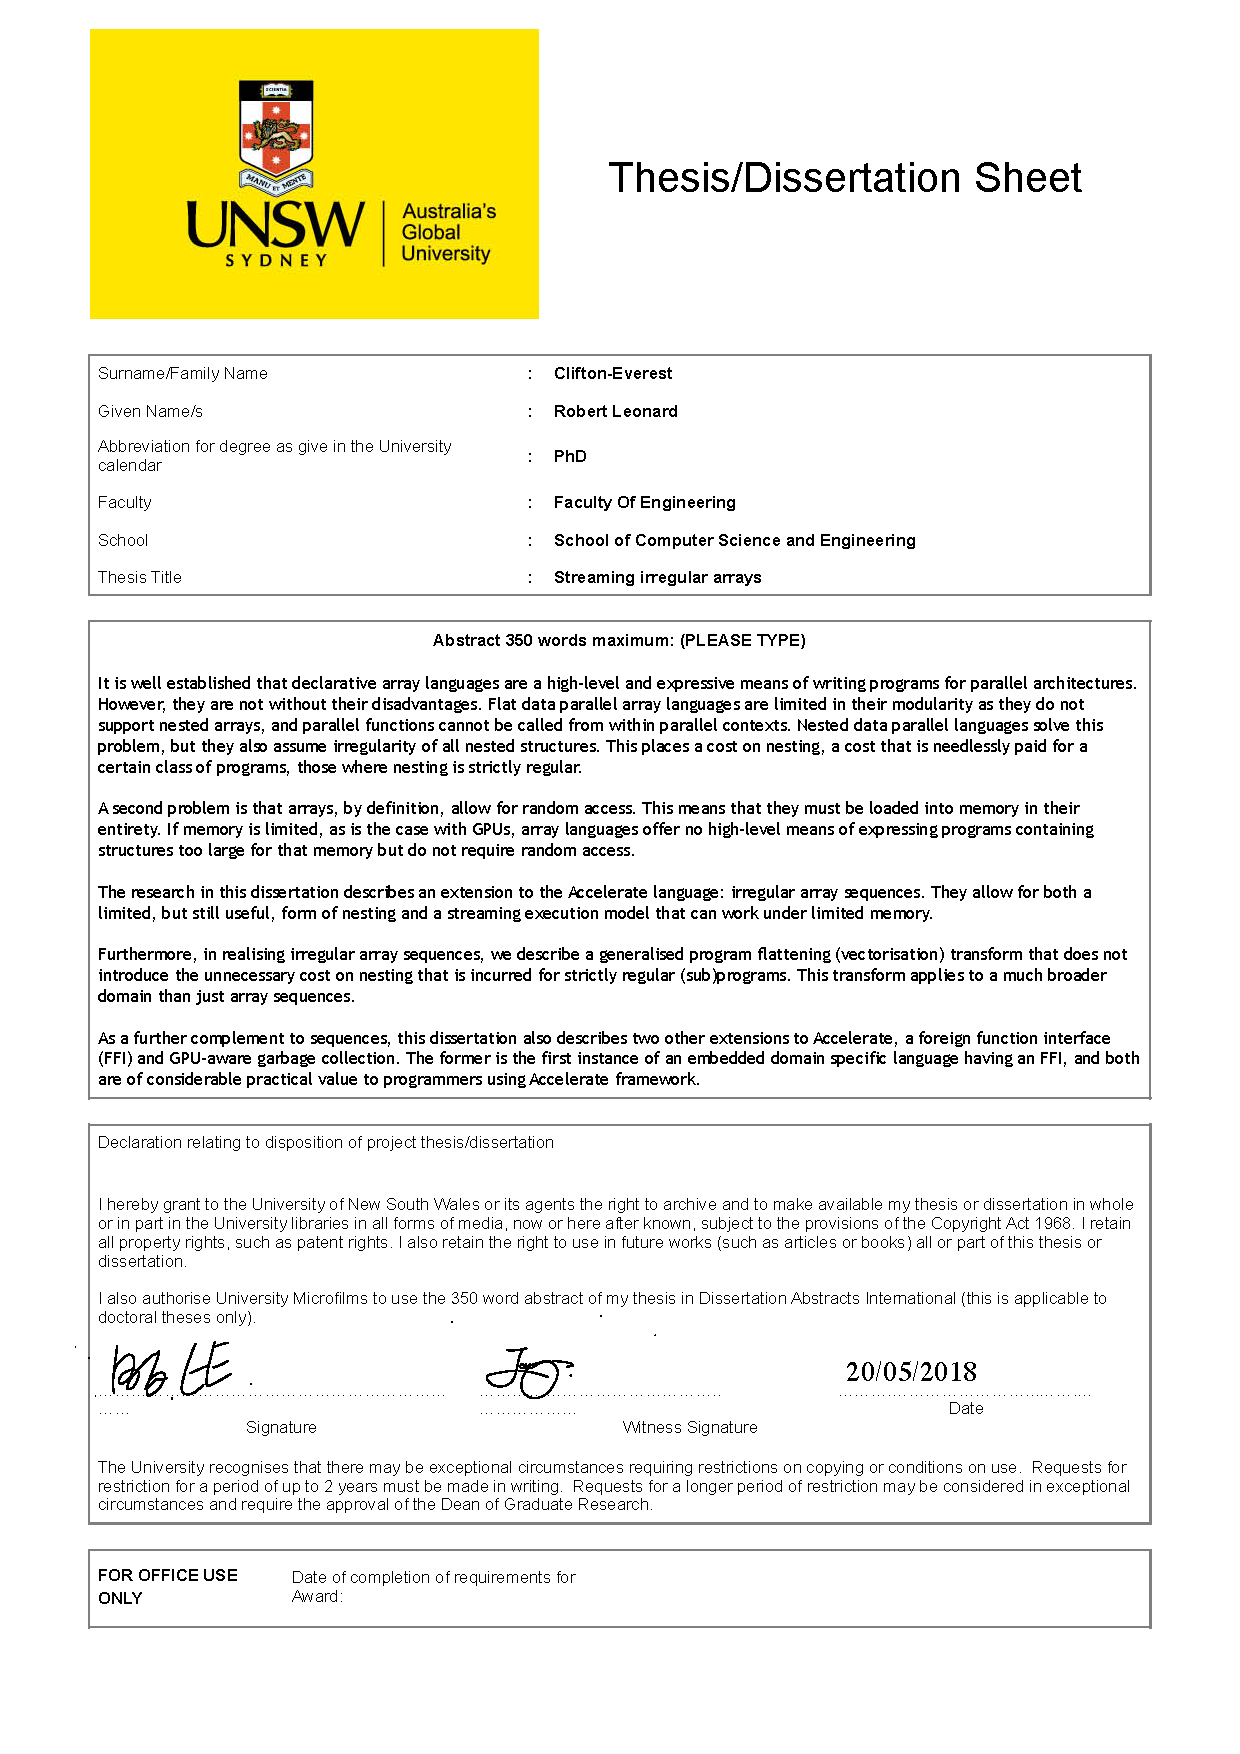
\includepdf{images/thesisdissertation_sheet.pdf}
\pagebreak
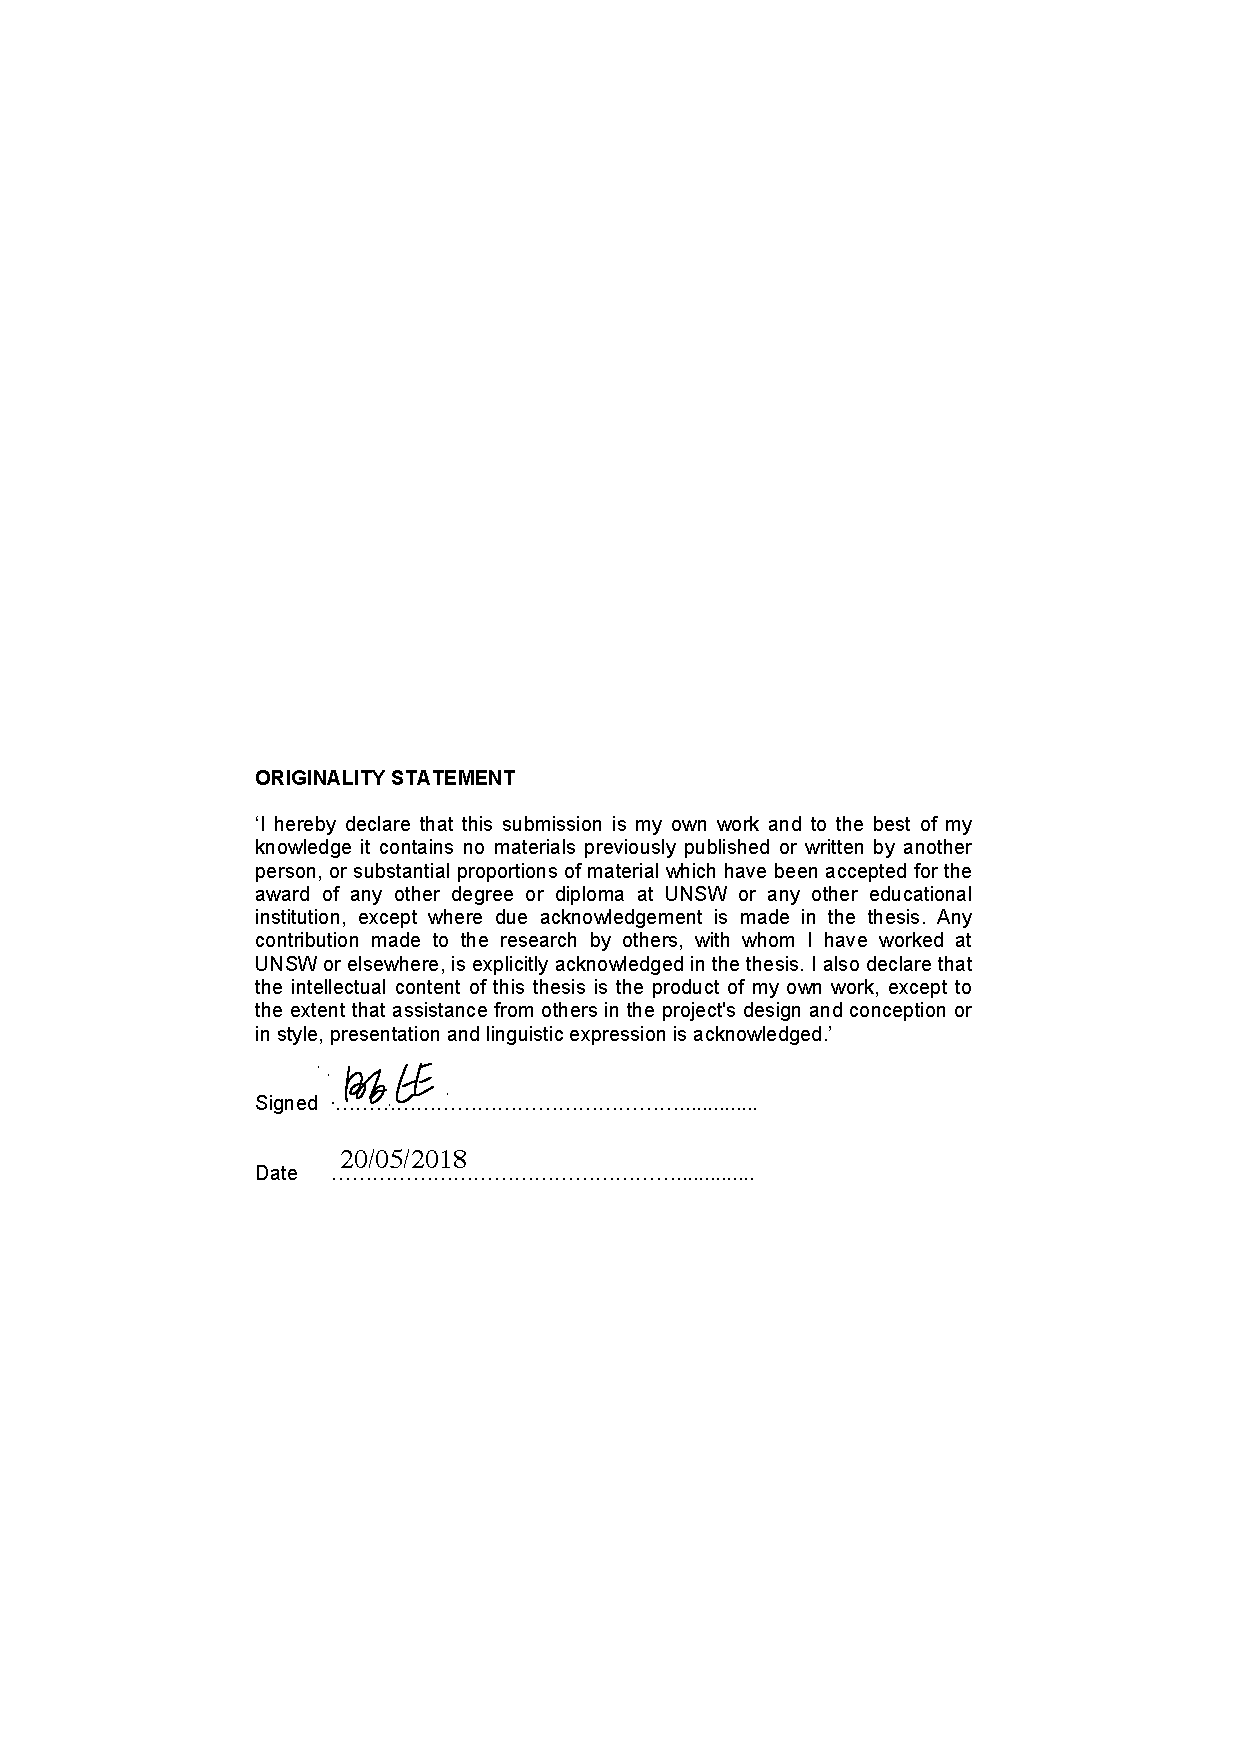
\includepdf{images/originalitystatement.pdf}

\cleardoublepage
\phantomsection
\addcontentsline{toc}{chapter}{Contents}
\tableofcontents\markboth{Contents}{Contents}

\cleardoublepage
\phantomsection
\renewcommand{\listfigurename}{Figures}
\addcontentsline{toc}{chapter}{\listfigurename}
\listoffigures\markboth{\listfigurename}{\listfigurename}

% \cleardoublepage
% \phantomsection
% \addcontentsline{toc}{chapter}{\lstlistlistingname}
% \lstlistoflistings\markboth{\lstlistlistingname}{\lstlistlistingname}
% \addtocontents{lol}{\vspace{10pt}}

\cleardoublepage
\phantomsection
\renewcommand{\listtablename}{Tables}
\addcontentsline{toc}{chapter}{\listtablename}
\listoftables\markboth{\listtablename}{\listtablename}


\chapter{Abstract}
\markboth{Abstract}{}

It is well established that declarative array languages are a high-level and expressive means of writing programs for parallel architectures. However, they are not without their disadvantages. Flat data parallel array languages are limited in their modularity as they do not support nested arrays and parallel functions cannot be called from within parallel contexts. Nested data parallel languages solve this problem but they also assume irregularity of all nested structures. This places a cost on nesting, a cost that is needlessly paid for a certain class of programs, those where nesting is strictly regular.

A second problem is that arrays, by definition, allow for random access. This means that arrays must be loaded into memory in their entirety. If memory is limited, as is the case with GPUs, array languages offer no high-level means of expressing programs containing structures too large for available memory but that do not require random access.

The research in this dissertation describes an extension to the Accelerate language: irregular array sequences. It allows for both a limited, but still useful, form of nesting and for the writing and execution of streaming programs under limited working memory.

Furthermore, in realising irregular array sequences, we describe a generalised program flattening (vectorisation) transform that does not introduce the cost on nesting that is unnecessarily incurred for strictly regular (sub)programs. This transform is applicable to a much broader domain than just array sequences.

Complementing this extension, this dissertation also describes two other extensions to Accelerate, a foreign function interface (FFI) and GPU-aware garbage collection. The former is the first instance of an embedded domain specific language having an FFI.


\chapter{Acknowledgements}
\markboth{Acknowledgements}{}

\begin{center}
My supervisors, Gabi and Manuel, for their expertise and support throughout a long 5 years.

\qquad

My family, not for any expertise, but certainly for their support, for an even longer period.

\qquad

More broadly, the Programming Languages and Systems group at UNSW: Gabi, Manuel, Trevor, Amos, Ben, Liam, Zilin, and the many others who came and went in my time there. Their support and advice were invaluable. Being a member has been a formative experience for me. Sadly the group is coming to an end as its members move on to better opportunities. It will not, however, be forgotten. It has too great a legacy for that.

\end{center}

\chapter{Publications}
\markboth{Publications}{}

During the course of my research, I coauthored the following publications:

\begin{itemize}
\item \bibentry{CliftonEverest:2014:acc-ffi}
\item \bibentry{Madsen:2015}
\item \bibentry{CliftonEverest:2017:streaming}
\end{itemize}


\mainmatter

\let\oldchapter\chapter
\renewcommand{\chapter}[1]{\oldchapter{#1}\addthumb{#1}{}{white}{black}}

\chapter{Introduction}

\Exam{I found the introduction to the thesis to be extremely short. I would have loved to see
a little more about motivating the use of array languages, what the domain of
programs that can be expressed is and why this domain matters. Also the current
limitation of Accelerate should have been discussed in more details together with a
justification as to why the work in this thesis is necessary. In particular the need for
flattening of arrays should be clearly motivated upfront.}

\finaltodo{Move material from background to here? Come up with simple example?}

A programmer wanting to take advantage of the immense processing power provided by modern parallel hardware has a common but difficult choice to make. They must decide what language to use. If they use a low-level language, it raises many questions: How time-consuming will that be? How much expert knowledge of the hardware is required?  What safety guarantees are there? Will programs be portable to the hardware that comes out next year? The answers to these questions are invariably: very, a lot, not many, and no.

Alternatively, they could use a high-level language. These are typically less time consuming to use, require less hardware specific knowledge, give greater safety guarantees, and can offer portability, provided there is a compiler for the target platform. They are, however, not often capable of generating native code with the desired performance properties.

Array languages have proven a robust compromise to this problem. They lift the level of abstraction beyond that of a low-level language, but still, most importantly, offer competitive performance. By expressing computations in terms of parallel arrays, there is a near limitless amount of parallelism available of which a sufficiently smart compiler can take advantage. Programs can be written by domain experts, as opposed to high-performance computing experts.

\finaltodo{More on array languages, disadvantages. Talk about programmer vs data representation}
That canonical example for such languages is the vector dot product, which may be written as something like:

\begin{lstlisting}
dotp xs ys = fold (+) 0 (zipWith (*) xs ys)
\end{lstlisting}

Two different array operations are used to compute the final result. @zipWith@ combines two arrays into one and @fold@ reduces the array down to a scalar value.

\finaltodo{more}
Some information it only really makes sense to represent in a flat structure. For example, a bitmap image is most naturally thought of as a 2D array of pixels. It is hard to think of a situation where it would be useful to treat an image as an array of rows of pixels. Similarly, nested structures make the most sense for other types of data. Text processing will usually treat text documents as arrays of lines of characters and rarely as a 2D grid of characters.

However, there is not always one natural structure. A matrix, for example, is could be treated as a 2D array in context, an array of rows in another, or an array of columns in yet another. This could be true even with the same program.

None of this takes into account how these structures are actually represented in memory. If a programmer chooses to represent a matrix as an array of rows, they may have to pay a performance penalty for that even though the underlying data is flat.

In this work, we contend that whether the programmer chooses to use nested structures should entirely be a decision based on usability. The programmer should be able to nest arrays without paying a penalty in the case that the underlying data can still be represented as flat array.

A leading language in this category is Accelerate. A highly expressive language rich with features and libraries. Embedded in Haskell, it offers combinators familiar to functional programmers, enabling them to write fast programs that closely resemble conventional Haskell programs.

\finaltodo{More on accelerate}

In this dissertation, we build upon Accelerate to widen the domain of programs that can be expressed within it. Not only that but, in doing so, we produce more general results that can be applied to any array language. Primarily, a program transformation for flattening nested parallelism that identifies and tracks the shape of nested structures.

This dissertation builds on existing work on Accelerate, and also array languages generally. Both prior to and during my contribution, numerous other researchers, also made many contributions. The research to which I have contributed is listed below. I explicitly state which work is my own:

\begin{itemize}
\item We have developed a new parallel structure in addition to the parallel array. Irregular arrays sequences offer a single level of nesting with greater modularity and controlled memory usage (Chapter~\ref{chap:motivation}).
\item I developed a novel extension to Blelloch's flattening transform~\cite{Blelloch:compiling1988,Blelloch:nesl1995} that identifies regular (sub)computations and transforms them according to different rules than irregular computations. By doing this I was able to take advantage of the greater efficiency afforded by regular computations, but fall back to less efficient methods when computations are irregular (Chapter~\ref{chap:theory}).
\item I implemented a system for treating the memory on Graphics Processing Units (GPUs) as a cache for GPU computations. A programmer using Accelerate with this feature does not have to be as concerned about their programs working memory fitting into the limited memory of the GPU (Section~\ref{sec:gpu-gc}).
\item I developed an foreign function interface (FFI) for Accelerate. This was the first, to my knowledge, FFI for an embedded language. The technique for doing this applies to all deeply embedded languages with multiple execution backends. In Accelerate, it allows for highly optimised low-level libraries to be called from within a high-level Accelerate program and for Accelerate programs to be called from CUDA C programs (Section~\ref{sec:foreign}).
\end{itemize}

Before describing any of this work, however, we first introduce the background and context of our research in Chapter~\ref{chap:background}.

\chapter{Background}
\label{chap:background}

While Accelerate itself is a flat data-parallel language, its design was strongly inspired by the Nested Data Parallel (NDP) model of programming, in particular, the approach taken by \citet{Blelloch:compiling1988} involving program flattening or vectorisation. Furthermore, the sequence extension of Accelerate, which is one of the main topics of this thesis, brings Accelerate closer to that of a Nested Data Parallel language. Therefore, we will start with introducing the NDP programming model and the concept of program flattening (Section~\ref{sec:ndp}), before describing the Accelerate language and its implementation in Haskell (Section~\ref{sec:background-accelerate}).

While Accelerate abstracts over concrete architectures and has multiple backends, one that is of particular importance is the backend that targets Nvidia GPUs via the CUDA framework. The sequence extension provides a benefit to that backend, due to the memory limitations of GPUs, and we also introduce some other extensions specifically for it. Hence, we will also give a brief overview of CUDA (Section~\ref{sec:cuda}).

% Before we explore the contributions of this work, we will first give a brief overview of the concepts it is built upon, the context in which it exists, and the technologies on which it depends. More specifically, we will describe:

% \begin{itemize}
%   \item The Nested Data Parallel model of programming and the concept of program flattening, or vectorisation, that underlies it (\ref{sec:ndp}).
%   \item The CUDA framework for general purpose GPU programming (\ref{sec:cuda}).
%   \item The Accelerate language and its implementation in Haskell (\ref{sec:background-accelerate}).
% \end{itemize}

\section{The Nested Data Parallel (NDP) programming model}
\label{sec:ndp}

The Nested Data Parallel (NDP) programming model is the most general form of data parallelism. It allows for arbitrary nesting of parallel operations within other parallel operations, as well as parallel structures which contain other parallel structures. For example, arrays of arrays. It is an expressive, high level and modular method of parallel programming~\cite{Blelloch:1990vl}. A variety of different useful algorithms have been implemented in languages supporting this model~\cite{Blelloch:nbody94,Blelloch:delaunay96,Blelloch:connected94}.

Nested data parallelism (NDP) was first popularised by the \nesl{} language~\cite{Blelloch:nesl1995}, but it currently exists in many different languages, albeit in a restricted form in some. These include Proteus~\cite{proteus-frontiers95}, Futhark~\cite{Henriksen:2017futhark}, Nova~\cite{collins2013nova}, Manticore~\cite{Fluet:2007:manticore}, Lift~\cite{Steuwer:lift}, Copperhead~\cite{Catanzaro:copperhead}, Nikola~\cite{Mainland:nikola}, and Data Parallel Haskell (DPH)~\cite{Jones:2008uu}. These languages implement nested parallelism by a variety of means. Manticore has an execution model based on fork-join parallelism. Lift, Copperhead, and Nikola directly map nested parallel combinators to the parallel hierarchy of GPUs. The rest rely on a program transformation first described by \citet{Blelloch:compiling1988} that flattens nested parallel structures and operations while preserving program behaviour. This technique is the one we use in our work, so will describe it here.
% Originally, \nesl{} programs were intended to execute on vector computers. These were strictly SIMD in nature so a transform was needed that would remove nested parallel structures and nested parallel operations, while preserving program behaviour. While computer hardware has changed considerably since then, the transform itself still has much utility.

% This first description of what shall now be referred to as Blelloch's Transform transformed from \plisp \citep{Sabot:paralation}, a version of lisp with simple parallel collections, to Scan-Vector Lisp, a subset of common lisp with a vector type. However, it was only possible to apply it to a subset of the source language and only to simple primitive types. Subsequently Scan-Vector Lisp was replaced with the intermediate language \vcode \citep{Blelloch:vcode1990}, a stack based data-parallel language.

Blelloch's Transform works by having two distinct components. The first being a \emph{flattened array representation}, the second, program \emph{flattening}. We will address each of these in turn.

\subsection{Array representation}
\label{sec:background-representation}

Computing with nested arrays requires a means for representing the nested structure in the flat memory provided by the von Neumann model.

To give a simple example, suppose we have this nested array.
%
\begin{lstlisting}
{ {A,B,C}, {D,E}, {F,G,H,I}, {}, {J} }
\end{lstlisting}
%
It is an array of arrays. The immediately obvious way of representing this is with an array of pointers. Indeed, most contemporary languages represent nested arrays in this way. Note that this is distinct from multidimensional arrays. While one can treat, say, a 2D array as an array of arrays, the fact that each \emph{subarray} has to be the same length does not make it a true nested array structure.

So if an array of pointers allows us to represent arbitrary nested array structures, what is the problem? It lies in the fact that modern computer hardware is optimised for locality of reference. Having different (often small) parts of the structure spread over memory with pointers between them means that any operations performed over them have to continually chase pointers and access new areas of memory. This results in many cache misses and is unworkable in the context of high performance. In addition, allocating pointer-based structures involves numerous small allocations. This means construction and destruction is expensive, and, in the context of a garbage collector, longer GC pauses.

An alternative solution to this problem, proposed by \citet{Blelloch:compiling1988}, is to \emph{flatten} the array structure. With that representation, a nested array is split into a pair consisting of an array of \emph{segment descriptors} and an array of values. The example above is represented as:
%
\begin{lstlisting}
({3,2,4,0,1}, {A,B,C,D,E,F,G,H,I,J})
\end{lstlisting}
%
The segment descriptors in the \emph{segments} array hold the size of corresponding subarray. So, we know that the first subarray contains the first 3 elements of the values vector, the next subarray 2, the next 4, etc.

Further nesting levels can then be represented by adding additional segment descriptors. For example:
%
\begin{lstlisting}
{ { {A,B}, {C} },
  { {D,E}, {}, {F} } }
\end{lstlisting}
%
becomes,
%
\begin{lstlisting}
({2,3}, ({2,1,2,0,1}, {A,B,C,D,E,F}))
\end{lstlisting}


% In addition to flattening nested arrays, arrays of tuples can be represented by tuples of arrays. This gives the the same benefits of locality as nested array flattening.

The segment descriptors we have in both of these examples are what we will refer to as \emph{size segment descriptors}, as they hold the size of subarrays. However, they are somewhat limited. Many operations with arrays in this form have worse complexity than the pointer-based equivalent. In particular, indexing, one of the most basic array operations, is no longer constant time. For example, finding the element at index 3 of the subarray at index 2 of
%
\begin{lstlisting}
({3,2,4,0,1}, {A,B,C,D,E,F,G,H,I,J})
\end{lstlisting}
%
involves taking the size of all subarrays before the one at index 2 and adding them together. In this case that's $3+2=5$. Then we have to add on 3 to that, $5+3=8$. This gives us the index of @I@, which is what we want. In general, size segment descriptors require at $O(n)$ (where $n$ is the number of subarrays) work to perform indexing.

There is another form of segment descriptor that solves this problem. Instead of holding the size of each subarray, it holds the offset. So, for our first example,
%
\begin{lstlisting}
({0,3,5,9,9}, {A,B,C,D,E,F,G,H,I,J})
\end{lstlisting}
%
We will call these \emph{offset segment descriptors}. In general, it takes $O(1)$ work to index arrays in this form as we already know where the corresponding subarray is located in the values vector.

Another useful operation, calculating the size of a given subarray, is similarly constant time. Merely take the offset of the subarray and subtract from the offset of the next subarray. However, this does not work for the final subarray and requires accessing two different elements of the segments array, which can be a problem for fusion (more on that in Chapter~\ref{chap:implementation}).

Instead, the better choice is \emph{size-offset segment descriptors} where both the size and the offset are stored.
%
\begin{lstlisting}
({(3,0),(2,3),(4,5),(0,9),(1,9)}, {A,B,C,D,E,F,G,H,I,J})
\end{lstlisting}
%
This has the advantages of both representations, but does require twice as much memory to store the segment descriptors.

% The former can be translated into the latter by simply applying @scanl (+)@ to the segment descriptor.

It is worth noting that there are other, more complex, nested array representations in existence. In particular \citet{Lippmeier:replicate} describe one that introduces the concept of \emph{virtual segments}. They allow for arrays to be replicated without explicitly storing them more than once. This problem arises when trying to support higher-order nested parallelism: when arrays can store functions as values. In the context of this work, we do not support higher-order nested parallelism, so we will not explore it in detail.

\subsection{Flattening}

Flattening, or vectorisation, is a syntax-driven program transformation. When given a program as input it outputs a flat data-parallel program which is semantically equivalent but operates on a flattened array representation.

As an example, consider this simple program.
%
\begin{lstlisting}
foo xs = map (map (\x -> 2*x + 1)) xs
\end{lstlisting}
%
If we wanted to rewrite this by hand, such that it didn't rely on a nested @map@ and explicitly worked with one of the nested array representation described above, we would most likely end up with this.
%
\begin{lstlisting}
foo' xs = let (segs, vals) = xs
          in (segs, map (\x -> 2*x + 1) vals)
\end{lstlisting}
%
In this case, we are simply mapping $2x+1$ over the all the values in the nested array. It is trivial to see that @foo@ and @foo'@ are equivalent, modulo the data representation. Blelloch's flattening transformation is a method for producing these equivalent programs. It works by \emph{lifting} functions into vector space. That is, given some function
%
\begin{lstlisting}
f :: a -> b
\end{lstlisting}
%
it lifts it into the function
%
\begin{lstlisting}
f%$^\uparrow$% :: Vector a -> Vector b
\end{lstlisting}
%
operating over vectors. Of course, if @a@ or @b@ are already vectors~\footnote{In these examples, we are treating vectors and arrays as being the same thing. For now, that is acceptable, but we will refine our definitions of both of these things in the following section.} then this function will be working over the nested representation of the now nested vectors.

Going back to our example, if we will start by lifting the lambda term
%
\begin{lstlisting}[style=ndp]
Lift[|\x -> 2*x + 1|]
\end{lstlisting}
%
For a function, we need to remember the length of the vector it should return. For all lifted functions, the length of the result should be the same as length of the argument. So we keep track of the argument as part of the \emph{lifting context}.
%
\begin{lstlisting}[style=ndp]
\x -> Lift_x[|2*x + 1|]
\end{lstlisting}
%
We can then use lifted version of the binary operation @+@. We will call this @+@$^\uparrow$.
%
\begin{lstlisting}[style=ndp]
\x -> Lift_x[|2*x|] +%$^\uparrow$% Lift_x[|1|]
\end{lstlisting}
%
For constants, we have to @replicate@ that constant out over a new vector. So for @1@ and @2@, we replicate it out by the length of the lifting context.
%
\begin{lstlisting}[style=ndp]
\x -> replicate (length x) 2 *%$^\uparrow$% Lift_x[|x|] +%$^\uparrow$% replicate (length x) 1
\end{lstlisting}
%
All that leaves us with is lifting the variable @x@. In this case, no extra work needs to be done. We just leave it as @x@ as it refers to the vector bound as argument to in the lambda term\footnote{In general this is not always true. See Chapter~\ref{chap:theory} for an in-depth explanation of how variables are treated during the lifting process.}.
%
\begin{lstlisting}[style=ndp]
\x -> replicate (length x) 2 *%$^\uparrow$% x +%$^\uparrow$% replicate (length x) 1
\end{lstlisting}
%
This is now the lifted version of our lambda term. Going back to the complete function.
%
\begin{lstlisting}
foo xs = map (map (\x -> 2*x + 1)) xs
\end{lstlisting}
%
We want to use lifting to remove the nested @map@. We can do that by first lifting the inner @map@ into application of the lifted function.
%
\begin{lstlisting}
Lift[|map (\x -> 2*x + 1)|]
\end{lstlisting}
%
Because we're now lifting a term that is already a vector, we are lifting into the nested array representation.
%
\begin{lstlisting}[style=ndp]
\(segs, vals) -> (segs, Lift[|\x -> 2*x + 1|] vals)
\end{lstlisting}
%
Essentially, we are able to replace a @map@ with the application of the lifted version of its first argument to the values of its second. More generally, the \emph{lifting rule} for @map@ is
%
\begin{lstlisting}[style=ndp]
Lift[|map f|] = \(segs, vals) -> (segs, Lift[|f|] vals)
\end{lstlisting}
%
Continuing on with our example, we can substitute the result of \lstinline[style=ndp]{Lift[|\x -> 2*x + 1|]} into the lifted version of the inner @map@.
%
\begin{lstlisting}
\(segs, vals) -> (segs, (\x -> replicate (length x) 2 *%$^\uparrow$% x +%$^\uparrow$% replicate (length x) 1) vals)
\end{lstlisting}
%
For the outer @map@, we could perform much the same thing, if we wanted a lifted version of @foo@, but if we instead just want @foo@ to be \emph{flattened} then we can replace it with the function above. More generally, this equivalence will always hold
%
\begin{lstlisting}[style=ndp]
map f = Lift[|f|]
\end{lstlisting}
%
Using it we can rewrite programs with nested @map@s to remove any nesting.

A similar approach can be taken for other array combinators. All that is required is to have a version of that combinator that can operate over the segmented representation. However, this is problematic for @fold@s. If we want a  parallel @fold@ that assumes its first argument is associative, we have to have this lifting rule:
%
\begin{lstlisting}[style=ndp]
Lift[|fold f z arr|] = fold_seg f z Lift[|arr|]
\end{lstlisting}
%
For this combinator, we do not lift the @f@ or @z@ arguments, meaning they cannot contain any nested parallelism. This is a common restriction on NDP languages.

The combinator @fold_seg@ is a necessary one to support @fold@ in NDP languages. It performs a \emph{segmented} fold. It can be thought of as performing a fold for every subvector of a vector of vectors.
%
\begin{lstlisting}[style=ndp]
fold_seg :: (a -> a -> a)
         -> a
         -> (Vector (Int,Int), Vector a)
         -> Vector a
\end{lstlisting}
%

In Chapter~\ref{chap:theory} we will describe a more general form of flattening and formally specify these operations.
%

\subsection{Avoidance}
\label{sec:advancements}

% Following the discovery of the flattening transform, \citet{Blelloch:nesl1995} devised the language \nesl in order to offer a language simpler than \plisp. \plisp was an extension to Common Lisp and as such had semantics that were difficult to translate to parallel execution. Similarly to \plisp, \nesl used \vcode as the intermediate language to generate in its vectorisation process. This represented the first step toward a more complete NDP language.

% While we have covered the basic concepts of Blelloch's lifting transform and program flattening, it is worth taking note of a few of its limitations and the extensions that help overcome them.

% Firstly, other than arrays, we did not explore what other data types can be supported. In this work, we are primarily concerned with arrays and product types. But other work~\cite{Keller:trees,Chakravarty:more-types} demonstrates that support for sum types and recursive types is also possible. These require changes to the nested array representation.

% Supposing we had an array of sum types
% %
% \begin{lstlisting}
% {%$\alpha$% + %$\beta$%}
% \end{lstlisting}
% %
% One possible representation is two arrays of values and an array of boolean flags called the \emph{selector}.
% %
% \begin{lstlisting}
% {Bool} %$\times$%  %$\times$% 
% \end{lstlisting}
% %
% A false in the selector array means that value should come from the left value array; a true, from the right value array.

% Firstly, in the context of functional languages, a question that naturally arises is how well this technique works for higher-order functions? Both in sense of flattening programs containing them but also allowing arrays of functions. This is Higher-Order NDP~\cite{Leshchinskiy:higher}. The techniques that allow for this, in particular, closure conversion~\cite{Minamide:1996}, we will not explore in detail as we do not do this work in the context of a higher-order functional language. We are strictly concerned with first-order array programs.

One extension to flattening which is important to our work is \emph{vectorisation avoidance}, avoiding vectorisation where necessary. For example, in this simple function from above,
%
\begin{lstlisting}
foo xs = map (map (\x -> 2*x + 1)) xs
\end{lstlisting}
%
flattening resulted in
%
%
\begin{lstlisting}
\(segs, vals) -> (segs, (\x -> replicate (length x) 2 *%$^\uparrow$% x +%$^\uparrow$% replicate (length x) 1) vals)
\end{lstlisting}
%
Doing so results in many intermediate arrays. If vectorisation can be avoided for the term
%
\begin{lstlisting}
\x -> 2*x + 1
\end{lstlisting}
%
then it is not necessary to construct all the intermediate arrays. \citet{Keller:avoidance} describe a way of avoiding vectorisation by having a pre-vectorisation tagging phase tagging sub-computations that do not need to be vectorised. In Chapter~\ref{chap:theory} we will describe a different solution to vectorisation avoidance, but one that could be improved by taking ideas from \citet{Keller:avoidance}.

\subsection{Fusion}
\label{sec:fusion}

Even with vectorisation avoidance, flattened array programs typically still contain many intermediate arrays. The na\"ive compilation of them quickly drags down performance as much of the program's runtime is spent reading and writing values to and from memory. This problem is not unique to flattened array programs, but is prevalent in the domain of functional programming and  collection-oriented languages generally. These languages, by their very nature, produce more intermediate structures than necessary. They facilitate and encourage programs to be written in that style because of the compositionality it yields.

Fusion (or deforestation) attempts to alleviate this problem by combining adjacent transformations on structures to remove intermediate results. This has been studied extensively, both in the general area of functional programming~\cite{Wadler:1990ix,Meijer:bananas,Gill:1993de,Coutts:stream-fusion} and specifically for arrays~\cite{Chakravarty:array-fusion,Lippmeier:Guiding,McDonell:acc-optim,Lippmeier:flow-fusion}.

For simple cases, fusion can be achieved by basic first-order term rewrites. For example, the rule
%
\begin{lstlisting}
map f (map g) = map (f . g)
\end{lstlisting}
%
removes the intermediate structure from applying @map@ to the result of another @map@. However, this does not work in the presence of let-bindings, which may obscure chains of @map@s, and there is no clear way to remove the intermediate structure in expressions of the form:
%
\begin{lstlisting}
fold f z (map f xs)
\end{lstlisting}
%
In this case, we need a more general approach.

On such approach is simple and well known~\cite{Claessen:obsidian-expressive,Guibas:1978jh,Elliott:2003ug}: represent an array by its size and a function mapping indices to their corresponding values. Fusion then becomes an automatic property of the data representation. This method is used successfully to optimise purely functional array programs in Repa~\cite{Keller:Repa,Lippmeier:Guiding} and Accelerate.

However, a straightforward implementation of this approach results in a loss of \emph{sharing}, which was a problem in early versions of Repa~\cite{Lippmeier:Guiding}. For example, consider the following program:
%
\begin{lstlisting}
let xs = {...}
    ys = map f xs
in zipWith g ys ys
\end{lstlisting}
%
Every access to an element @ys@ will apply the (arbitrarily expensive) function @f@ to the corresponding element in @xs@. It follows that these computations will be done \emph{at least} twice, once for each argument in @g@, quite contrary to the programmer's intent. Accelerate's solution to this problem is not to fuse such terms. However, this can prevent fusion in cases where it may actually be the most efficient choice. We will explore this problem in greater depth in Section~\ref{sec:Optimisation}.

\section{Accelerate}
\label{sec:background-accelerate}

As part of our work, we extend the array language \emph{Accelerate}. What follows is an overview of Accelerate from the perspective of a user of the language: how to write programs, how they are executed, what its limitations are, etc. In the subsequent section (\ref{sec:acc-internals}) we will explore some of the internal design of the compiler.

\subsection{Overview}
\label{sec:acc-intro}

Accelerate is a parallel array language consisting of a carefully selected set of operations (combinators) on multidimensional arrays, which can be compiled efficiently to bulk-parallel SIMD hardware. It is \emph{deeply embedded} in Haskell, meaning that we write Accelerate programs with (slightly stylised) Haskell syntax.

Accelerate code embedded in Haskell is not compiled to SIMD code by the Haskell compiler; instead, the Accelerate library includes a \emph{runtime compiler} that generates parallel SIMD code at application runtime. Currently, there are two complete code-generation backends, one for multi-core CPUs and one for Nvidia GPUs. Both share a significant code base owing to the fact they both work via LLVM.

The collective operations in Accelerate are based on the scan-vector model~\citep{Chatterjee:1990vj,Sengupta:2007tc}, and consist of multi-dimensional variants of familiar Haskell list operations such as @map@ and @fold@, as well as array-specific operations such as index permutations.

For example, this is a simple vector dot-product function written in Accelerate:
%
\begin{lstlisting}
dotp :: Acc (Vector Float) -> Acc (Vector Float) -> Acc (Scalar Float)
dotp xs ys = fold (+) 0 ( zipWith (*) xs ys )
\end{lstlisting}
%
The function @dotp@ consumes two Accelerate computations. The type @Acc a@ can be interpreted to mean an Accelerate computation producing an @a@. So, in this case, each of the argument computations produces a one-dimensional array (@Vector@) of @Float@ when evaluated. This function then returns a new computation which, when evaluated, yields a single (@Scalar@) result as output.

The Accelerate code for @dotp@ is almost identical to what we would write in standard Haskell over lists and is certainly more concise than an explicitly GPU-accelerated or SIMD-vectorized\footnote{That is, a program utilising the SSE/AVX instruction set extensions for x86 processors.} low-level dot-product, while still compiling to efficient code~\citep{Chakravarty:acc-cuda,McDonell:acc-optim,McDonell:2015:acc-llvm}.

The functions @zipWith@ and @fold@ are defined by the Accelerate library and have \emph{highly parallel} semantics, supporting up to as many parallel threads as data elements. The type of @fold@ is:
%
\begin{lstlisting}
fold :: (Shape sh, Elt e)
     => (Exp e -> Exp e -> Exp e)
     -> Exp e
     -> Acc (Array (sh:.Int) e)
     -> Acc (Array sh e)
\end{lstlisting}
%
This definition exposes some other important components to the language. The type class @Shape@ indicates that a type is admissible as an array \emph{shape}. In the simple terms, this means that it must be one of 1D, 2D, 3D, etc. The valid members of the @Shape@ class are:
%
\begin{lstlisting}
instance Shape Z
instance Shape sh => sh :. Int
\end{lstlisting}
%
This allows for arbitrary rank shapes to be built at the type level as snoc-lists~\citep{Keller:Repa,Chakravarty:acc-cuda}. Accelerate defines some synonyms for common shapes:
%
\begin{lstlisting}
type DIM0 = Z
type DIM1 = DIM0:.Int
type DIM2 = DIM1:.Int
type DIM3 = DIM2:.Int
type DIM4 = DIM3:.Int
...
\end{lstlisting}
%
The shape @Z@ is the scalar shape. An array of shape @Z@ is called a scalar array and only has 1 element. This was the result type of @dotp@, via this synonym:
%
\begin{lstlisting}
type Scalar = Array Z
\end{lstlisting}
%
Similarly, a vector is just a 1D array.
%
\begin{lstlisting}
type Vector = Array DIM1
\end{lstlisting}
%

Going back to @fold@, we also have the @Elt@ type class. This indicates that a type is admissible as an element of an array. It encompasses many primitive types including:
%
\begin{lstlisting}
instance Elt Int
instance Elt Float
instance Elt Double
instance Elt Char
instance Elt Bool
instance Elt Word8
instance Elt Word16
instance Elt Word32
...
\end{lstlisting}
%
In addition, tuples of arity up to 16 are admissible.
%
\begin{lstlisting}
instance (Elt a, Elt b)               => Elt (a,b)
instance (Elt a, Elt b, Elt c)        => Elt (a,b,c)
instance (Elt a, Elt b, Elt c, Elt d) => Elt (a,b,c,d)
...
\end{lstlisting}
%
In fact, @Elt@ is user extensible via representation types. We won't cover how that works in detail here, but the salient point is that @Elt@ is a truly open type class.

The type signature for @fold@ also shows how Accelerate is stratified into two different levels. We have already seen collective \emph{array computations}, represented by terms of the type @Acc t@, but there is also \emph{scalar expressions}, represented by terms of type @Exp t@. More concretely, values of type @Acc t@ and @Exp t@ do not execute computations directly, rather they represent abstract syntax trees (ASTs) constituting a computation that, once executed, will yield a value of type @t@. Collective operations comprise many scalar operations which are executed in data-parallel, but scalar operations \emph{cannot} initiate collective operations. This stratification helps to statically exclude nested parallelism. We will explore in more detail what this restriction means for modularity in Chapter~\ref{chap:motivation}.

\subsubsection{Operations}

Accelerate offers many different array operations. We give a brief overview of the key ones here.

@map@ and @zipWith@ behave in much the same way as those same operations over lists. For multidimensional arrays @zipWith@ yields an array of the minimum shape of all dimensions in the array. For example, if array @a@ has extent
%
\begin{lstlisting}
Z :. 5 :. 4
\end{lstlisting}
%
and array @b@ has extent
%
\begin{lstlisting}
Z :. 3 :. 6
\end{lstlisting}
%
then the result of
%
\begin{lstlisting}
zipWith f a b
\end{lstlisting}
%
Will have extent
%
\begin{lstlisting}
Z :. 3 :. 4
\end{lstlisting}
%

The @fold@ we used in @dotp@ works by folding along the inner dimension. One can view this as performing a series of many folds. Every vector along the inner dimension is reduced.

@generate@ is the most general array operation.
%
\begin{lstlisting}
generate :: (Shape sh, Elt e) => Exp sh -> (Exp sh -> Exp e) -> Array sh e
\end{lstlisting}
%
It constructs an array of the given extent using the supplied function to fill its elements. For exammple:
%
\begin{lstlisting}
evens :: Exp Int -> Acc (Vector Int)
evens sz = generate (index1 sz) (\ix -> unindex ix * 2)
\end{lstlisting}
%
This example also shows the scalar operations @index1@ and @unindex1@.
%
\begin{lstlisting}
index1 :: Exp Int -> Exp DIM1
index1 :: Exp DIM1 -> Exp Int
\end{lstlisting}
%
They convert between @Int@s and @DIM1@s.

Similarly, we have the operations @lift@ and @unlift@. They are generic functions for converting tuples in the meta-language to tuples in the object language, and vice versa. Expressing these functions in the Haskell type system is tricky, but one can think of them in this form.
%
\begin{lstlisting}[style=ndp]
lift   :: (Exp e_1, Exp e_2, ..., Exp e_n) -> Exp (e_1, e_2, ..., e_n)
unlift :: Exp (e_1, e_2, ..., e_n)         -> (Exp e_1, Exp e_2, ..., Exp e_n)
\end{lstlisting}
%

Various forms of prefix sum (scan) are supported. One of the main ones is, @scanl@, for performing a left scan.
%
\begin{lstlisting}
scanl :: (Shape sh, Elt e)
      => (Exp e -> Exp e -> Exp e)
      -> Exp e
      -> Acc (Array (sh:.Int) e)
      -> Acc (Array (sh:.Int) e)
\end{lstlisting}
%
It too is similar in semantics to @scanl@ in Haskell. Like @fold@, it assumes the binary operation is associative and works over the inner dimension.

Other array and scalar operations we will introduce as the need arises.


\subsection{Internals}
\label{sec:acc-internals}

The Accelerate compilation pipeline has 4 major stages and uses two different syntax representations. The stages are:
%
\begin{itemize}
%
\item Sharing recovery -- Converts the higher-order abstract syntax (HOAS) into first-order syntax with De Bruijn indices and also recovers sharing.
%
% \item Segment rewriting -- If necessary, will rewrite explicit segment operations such that segment descriptors are converted into the right format. This will be covered in more depth below. For now, it is just another compilation stage.
%
\item Fusion and optimisation -- Tries to minimise unnecessary array traversals and optimises for optimal code generation. This produces an AST with explicit delayed arrays.
%
\item Code generation -- Generates LLVM IR from the AST and passes it off to the LLVM compiler. This stage is different for each backend. The CPU backend generates x86 binaries (with vector instructions) and the PTX backend generates PTX code for CUDA capable GPUs.
%
\item Execution -- Schedules and executes the computations on the target hardware.
\end{itemize}
%

The first of these stages we won't explore in detail, as it is not a concern of this work. It is sufficient to understand it as the process that produces the first-order syntax in Listing~\ref{lst:acc-ast} from the programmer-friendly higher-order syntax. See \citet{McDonell:acc-optim} for details on how this stage of the pipeline works.

The fusion and optimisation stage we will discuss in Chapter~\ref{chap:implementation} where we will build upon the previous work described in \citet{McDonell:acc-optim}.

Code generation is not discussed in detail as it is not a focus of this work. See \citet{McDonell:2015:acc-llvm} for how LLVM is generated from the AST in Listing~\ref{lst:acc-ast}.

Execution will be covered in Chapter~\ref{chap:implementation} where we build upon the previous work\cite{McDonell:acc-optim,McDonell:2015:acc-llvm,Chakravarty:acc-cuda}.

\subsubsection{Abstract Syntax Tree}

The abstract syntax tree for the core Accelerate syntax is given in \ref{lst:acc-ast} for the @Acc@ stratum and \ref{lst:exp-ast} for @Exp@. These ASTs are all parameterised by the recursive step @acc@.

\begin{aside}
\begin{center}
\textbf{Aside: Tying the recursive knot}
\end{center}

By having the recursive step as a parameter, rather than simply making a GADT recursive, we are able to annotate it differently in different contexts. For our AST, not only can we recover the recursion with @OpenAcc@
%
\begin{lstlisting}
newtype OpenAcc aenv a = OpenAcc (PreOpenAcc OpenAcc aenv a)
\end{lstlisting}
%
we are also able to, for example, annotate it with labels for user-debugging,
%
\begin{lstlisting}
data LabelledAcc aenv a = LabelledAcc String (PreOpenAcc OpenAcc aenv a)
\end{lstlisting}
\end{aside}

The second parameter is a snoc-list, represented using left-nested tuples, of the environment. The @Alet@ AST form allows for new variables to be introduced into the environment and @Avar@ extracts their values. @Idx@ is a typed De Bruijn index.
%
\begin{lstlisting}
data Idx env a where
  ZeroIdx :: Idx (env,a) a
  SuccIdx :: Idx env a
          -> Idx (env,b) a
\end{lstlisting}
%

We can see the relation between the @Exp@ and @Acc@ strata by looking at the definition of the @Generate@ constructor and expanding the type synonyms within it
%
\begin{lstlisting}
  Generate :: (Elt e, Shape sh)
           => PreOpenExp acc aenv () sh
           -> PreOpenFun acc aenv () (sh -> e)
           -> PreOpenAcc acc aenv (Array sh e)
\end{lstlisting}
%
we observe how both arguments are parameterised by the recursive @acc@ step and array environment but have closed scaler environments. We say that these term are open with respect to the array environment but closed with respect to the scalar environment.

Tuples are represented with a snoc-list, like the environment.

In the case of @Index@, we see how the recursive step can be embedded in @Exp@ terms. While the type system does not enforce this, for most stages of the compilation we have as an invariant that any @Acc@ term embedded in @Exp@ must be an @Avar@. This way, scalar computations can access arrays previously computed but cannot compute further array operations.


\begin{lstlisting}[label=lst:acc-ast, caption={The first-order abstract syntax of the \texttt{Acc} level of Accelerate.}, style=haskell]
type Acc = OpenAcc ()
newtype OpenAcc aenv a = OpenAcc (PreOpenAcc OpenAcc aenv a)

data PreOpenAcc acc aenv a where
  Map      :: (Elt a, Elt b, Shape sh)
           => PreFun     acc aenv (a -> b)
           -> acc            aenv (Array sh a)
           -> PreOpenAcc acc aenv (Array sh b)

  ZipWith  :: (Elt a, Elt b, Elt c, Shape sh)
           => PreFun     acc aenv (a -> b -> c)
           -> acc            aenv (Array sh a)
           -> acc            aenv (Array sh b)
           -> PreOpenAcc acc aenv (Array sh c)

  Generate :: (Elt e, Shape sh)
           => PreExp     acc aenv sh
           -> PreFun     acc aenv (sh -> e)
           -> PreOpenAcc acc aenv (Array sh e)

  Fold     :: (Elt a, Shape sh)
           => PreFun     acc aenv (a -> a -> a)
           -> acc            aenv (Array (sh:.Int) a)
           -> acc            aenv (Array sh a)
           -> PreOpenAcc acc aenv (Array sh a)

  Avar     :: Arrays a
           => Idx aenv a
           -> acc aenv a

  Alet     :: (Arrays a, Arrays b)
           => acc            aenv     a
           -> acc            (aenv,a) b
           -> PreOpenAcc acc aenv     b

  Atuple   :: Arrays t
           => Atuple     acc aenv (TupleRepr t)
           -> PreOpenAcc acc aenv t
  ...
\end{lstlisting}

\begin{lstlisting}[label=lst:exp-ast, caption={The first-order abstract syntax of the \texttt{Exp} level of Accelerate.}]
type Fun = OpenFun ()
type PreFun acc = PreOpenFun acc ()
type OpenFun = PreOpenFun OpenAcc

data PreOpenFun acc env aenv f where
  Body :: Elt b
       => PreOpenExp acc env     aenv b

  Lam  :: (Elt a, Elt b)
       => PreOpenFun acc (env,a) aenv b
       -> PreOpenFun acc env     aenv (a -> b)

type Exp = OpenExp ()
type PreExp acc = PreOpenExp acc ()
type OpenExp = PreOpenExp OpenAcc

data PreOpenExp acc env aenv e where
  Index   :: (Shape sh, Elt e)
          => acc                aenv (Array sh e)
          -> PreOpenExp acc env aenv sh
          -> PreOpenExp acc env aenv e

  Let     :: (Elt a, Elt b)
          => PreOpenExp acc env     aenv a
          -> PreOpenExp acc (env,a) aenv b
          -> PreOpenExp acc env     aenv b

  Var     :: Elt e
          => Idx env e
          -> PreOpenExp env aenv e

  Tuple   :: (Elt t, IsTuple t)
          => Tuple      acc env aenv (TupleRepr t)
          -> PreOpenExp acc env aenv t
  ...

data Tuple acc env aenv t where
  NilTup  :: Tuple acc env aenv ()

  SnocTup :: Elt a
          => Tuple      acc env aenv t
          -> PreOpenExp acc env aenv a
          -> Tuple      acc env aenv (t,a)
\end{lstlisting}
%

\section{CUDA}
\label{sec:cuda}

The CUDA (Compute Unified Device Architecture)\cite{cuda} programming environment provides libraries and extensions to LLVM, C and C++, as well as Fortran. They enable programs to be written for and executed on NVIDIA GPUs.

The Accelerate compiler I described above has a backend that generates LLVM IR which is subsequently compiled by the CUDA framework. For explanation, however, examples are given in CUDA C as that is how the majority of programmers use CUDA.

Concretely, a C programmer wanting to take advantage of a CUDA capable GPU would annotate functions in their program with special directives indicating they are intended for GPU execution. When run through the \emph{nvcc} compiler any function annotated with these directives will be compiled into code in the Parallel Thread Execution (PTX) instruction set. These annotated functions, known as kernels, can be called with a special notation that specifies how they should be scheduled, in particular, how many multiprocessors to use. The code in~\ref{lst:cuda} shows a simple example where two vectors of size $N$ are added together by $N$ threads.
%
\begin{lstlisting}[language=C, label=lst:cuda, caption={Adding two $N$ length vectors in CUDA C\citep{cuda}}]
// Kernel definition
__global__ void VecAdd(float* A, float* B, float* C)
{
    int i = threadIdx.x;
    C[i] = A[i] + B[i];
}

int main()
{
    ...
    // Kernel invocation with N threads
    VecAdd<<<1, N>>>(A, B, C);
    ...
}
\end{lstlisting}
%
This example corresponds to this simple Haskell function
%
\begin{lstlisting}
vecAdd :: [Float] -> [Float] -> [Float]
vecAdd = zipWith (+)
\end{lstlisting}

In general, it is reasonably clear how trivially parallel programs, like those that only rely on @map@s and @zipWith@s, can be implemented in CUDA C. It is less clear, however, how to map other high-level combinators (for example @fold@ and @scan@) to a corresponding GPU kernel. To do such things, the programmer has to concern themselves with the hierarchy of the GPU. Kernels are executed by threads in SIMD groups called warps arranged in thread blocks. Different threads in the same block can coordinate by fast shared memory, whereas threads in different blocks can only coordinate via the slower global memory. To further complicate the programmer's task, there are also issues of SIMD divergence and memory access patterns. All of these must be taken into account to achieve optimal performance.

% \paragraph{Dynamic parallelism}
% A particular feature of the CUDA programming model that is worth noting is \emph{dynamic parallelism}~\cite[Appendix D]{cuda}. Dynamic parallelism in this case being the ability to create and launch new kernels from within one that is already running. While at first glance this may appear to provide nested parallelism, it is not without limitations. There is an upper limit on the nesting depth of 24 and each new level of nesting requires an extra 150MB of device memory. While this would be suitable for algorithms that had a small fixed depth of nested parallelism, it would not work at all for algorithms like the Barnes-Hut algorithm for n-body simulation \citep{barnes:1986}. Such algorithms require dynamic trees where the parallel nesting depth is equivalent to the depth of the tree.

The difficulties of directly programming through the low-level CUDA framework is what inspired many languages, compilers, and frameworks that try to lift the level of abstraction. This was and is the motivation for Accelerate.

% \subsubsection{Simultaneous substitution}


% How is this helping to motivate nesting in any way? -=chak
%
% Furthermore, the typical solution to our first problem (\S\ref{sec:problem_1})
% is by use of the \emph{flattening transform}~\citep{Blelloch:compiling1988},
% which converts source programs using nested data-parallelism into ones using
% just flat data-parallelism. Unfortunately, the flattening transform often
% results in programs which suffer a severe blow-up in their asymptotic time and
% space complexity~\citep{Lippmeier:replicate,Palmer:piecewise}, limiting their
% utility and further exacerbating the problem of running our programs on
% memory-constrained devices.


% \section{Other GPGPU Languages}

% There are numerous languages other than Accelerate, both embedded and not, that are intended to provide easier ways of GPU programming. Here is an overview of a selection of them, chosen for having similar goals and features to Accelerate. A particular focus is on the degree of nested parallelism they provide.

% \paragraph{Vertigo}
% Vertigo \citep{Elliott:Vertigo} was an early purely functional Haskell-embedded language for 3D graphics with an optimising compiler for DirectX 9 capable GPUs. It was restricted to generating and shading shapes. While it did compile for the GPU, its restrictive problem domain makes it unsuitable for general purpose programming. However, it was the inspiration for subsequent Haskell-embedded GPGPU languages.

% \paragraph{Nikola}
% Nikola \citep{Mainland:nikola}, in its design, is the most similar to Accelerate of all these languages. Like Accelerate it compiles to CUDA C and features the standard collection of data-parallel combinators (@map@, @fold@, @zip@, etc.). However, it only supports constructs for which the size of the output array can be statically inferred. As such, it does not support @generate@ or @replicate@ and can only compile to a single kernel. If a user needs to perform a computation that requires multiple kernels they are left having to schedule this themselves.

% \paragraph{Obsidian}
% Based on the concept of connection patterns, Obsidian \citep{Claessen:obsidian,Claessen:obsidian-expressive} provides a GPGPU programming environment that aims to make GPU programming easier, without losing fine grain control of GPU resources. Again a Haskell-embedded language, it is based on the hardware design language Lava \citep{Bjesse:lava} and compiles to CUDA code. Unlike Accelerate, Obsidian is intended to offer a more low-level programming experience, with the programmer having direct control over things like memory layout and where parallelism is introduced. It bears more similarity to the hardware design language on which it is based than any data parallel language. While it is sufficiently powerful enough to allow for general purpose programming, it is still limited in the fact that functions in the language can only take one array as input, and one as output. Additionally, the size of an array is limited to maximum number of threads a CUDA thread block can legally contain (1024 for the latest CUDA-capable hardware). Like Nikola above, it can also only compile to a single CUDA kernel.

% \paragraph{Copperhead}
% Unlike the three languages above, Copperhead \citep{Catanzaro:copperhead} is embedded in Python. Like Accelerate and Nikola, it is implemented as a data parallel language with constructs like @map@, @reduce@ and @zip@. Unlike Accelerate however, it does support a degree of nested data-parallelism. This is achieved not through a flattening or vectorisation transform like the languages of \nesl \citep{Blelloch:nesl1995} and Data Parallel Haskell \citep{Jones:2008uu} (see \ref{sec:ndp} below), but by statically mapping nested programs onto the parallel hierarchy. As such the programmer has to be specify how they want nested parallel subcomputations to be mapped. The default is to simply replace them with a sequential implementation.

% \paragraph{NDP2GPU}
% NDP2GPU, described by \citet{bergstrom:ndp2gpu}, compiles \nesl \citep{Blelloch:nesl1995}  down to CUDA. The frontend of \nesl supports complete nested data parallelism, which allows the compilation of NDP programs for the GPU. This is in contrast to all the languages above. However, as the authors note, its performance is still distinctly below that of hand-written CUDA code. In addition, unlike Accelerate, only a basic form of @map@/@map@ fusion is supported.

% \paragraph{CuNesl}
% CuNesl \citep{Zhang:2012jl} is another compiler for compiling \nesl to CUDA C. It is distinct from NDP2GPU in that it supports a transformation for eliminating recursive function calls by converting them to while-loops; recursive functions being costly to execute on GPUs. While it does support eliminating more than just simple tail-recursion, it still does not eliminate all recursive calls; i.e. it can only work on recursive functions of the form shown in \ref{lst:cunesl-example} and functions that can be trivially transformed into this form. This is in contrast to all the other languages listed in this section as they either do not support recursive functions at all, in the case of Haskell-embedded languages, or simply do not support efficient execution of them, as is the case with Copperhead and NDP2GPU.

% \begin{lstlisting}[label=lst:cunesl-example, caption={The general form of a recursive function that can be transformed by CuNesl. P1..P4 are blocks that do not contain recursive calls.}]
% void fun(...) {
%   P1()
%   if (branch) {
%     P2();
%     return;
%   } else {
%     P3();
%     fun(...);
%     ...
%     P4();
%     return;
%   }
% }
% \end{lstlisting}

% While it may seem highly restrictive that Accelerate and the other embedded languages do not support recursive functions, the very fact that they are embedded allows for meta-programming. Recursive functions can be replaced by functions in the host language that generate the --- typically very large --- unfolded version of the function in the object language.

% \paragraph{Barracuda}
% Barracuda \citep{Larsen:baracuda} is another language embedded within Haskell. It is, however, more primitive than Obsidian, Nikola and Accelerate, as it only features the most basic array primitives. The fact it lacks a @scan@ primitive means it cannot implement a lot of real-world data-parallel algorithms \citep{Blelloch:1990vl}. It is also distinct from these other languages because it is intended for offline compilation and inclusion in high performance C++ applications. It does not provide any mechanism for runtime code generation and compilation. This neatly side steps the issues of overhead faced by these languages.

% While the distinction between libraries and languages is not always clear (in the case of embedded languages at least), the above list focuses on languages for GPU programming. There are numerous libraries that can take advantage of the increased performance of running code on the GPU. Thrust \citep{Bell:thrust} is a parallel algorithms library designed to resemble the C++ Standard Template Library (STL). \citet{Sato:Skeletal-fusion} demonstrated a skeletal parallel programming framework for writing GPGPU applications. Like Accelerate, it features a fusion mechanism.

% \TODO{Go through some more C++ libraries. Doesn't need a lot of detail.}

\chapter{Sequences}
\label{chap:motivation}

In this chapter, we introduce \emph{irregular array sequences} as an extension to Accelerate. This extension represents a novel way of overcoming two major limitations of flat data parallelism. We first explore these limitations in depth (Section~\ref{sec:limitations}) before describing the extension itself (Section~\ref{sec:sequences}).

% This extension adds to the expressiveness of Accelerate in a significant way, but requires both a new program transformation, described in Chapter~\ref{chap:theory} and other optimisations, described in Chapter~\ref{chap:implementation}.

% Before describing the core theory (Chapter \ref{chap:theory}) and the implementation (Chapter \ref{chap:implementation}) of our work, it is important to first address \emph{why} what we have done is useful. As discussed above, we propose that even a limited form of nesting allows for greater expressiveness of array programs. In addition, if that nesting is in the form of sequences of arrays we get the benefit of greater control of memory usage and the ability to automatically schedule out of core algorithms.

% We will motive the work by presenting a simple API extension to Accelerate that adds sequences to the language. We will also show through a series of examples how this extension enables the writing of programs that either would have been hard to write in a modular way or not possible to write at all.

\section{Limitations of array-based flat data parallelism}
\label{sec:limitations}
While flat data parallel array languages, like Accelerate, offer a powerful, high-level means of parallel programming, they are not without drawbacks. In this work, we focus on two of the major ones. Firstly, the reduction of modularity that results from strictly flat data-parallelism (Section~\ref{sec:problem_1}), and, secondly, the memory usage that arises from the inherent random access nature of arrays (\ref{sec:problem_2}).

\subsection{Modularity}
\label{sec:problem_1}

Recall the simple dot product example from Section~\ref{sec:acc-intro}:
%
\begin{lstlisting}
dotp :: Acc (Vector Float) -> Acc (Vector Float) -> Acc (Scalar Float)
dotp xs ys = fold (+) 0 ( zipWith (*) xs ys )
\end{lstlisting}
%
We would like to re-use this function to implement a matrix-vector product, by applying it to each row of the input matrix:
%
\begin{lstlisting}
mvm%$_\texttt{ndp}$% :: Acc (Matrix Float) -> Acc (Vector Float) -> Acc (Vector Float)
mvm%$_\texttt{ndp}$% mat vec =
  let Z :. m :. _ = shape mat
  in  generate (Z:.m) (\row -> the $ dotp vec (slice mat (row :. All)))
\end{lstlisting}
%
Here, @generate@ creates a one-dimensional vector containing @m@ elements by applying the supplied function at each index in data-parallel. At each index, we
extract the appropriate row of the matrix using @slice@, and pass this to our existing @dotp@ function together with the input vector.

The \inl{slice} operation is a generalised array indexing function which is used to cut out \emph{entire dimensions} of an array. In @slice mat (row :. All)@,
we extract \inl{All} columns at one specific \inl{row} of the given
two-dimensional matrix, resulting in a one-dimensional vector. @the@ is a specialised form of indexing for extracting the value from a scalar array.
%
\begin{lstlisting}
the :: Acc (Scalar a) -> Exp a
the = (! Z)
\end{lstlisting}
%

Unfortunately, since both @generate@ and @dotp@ are data-parallel operations,
this definition requires nested data-parallelism and is thus not permitted.\footnote{By not permitted, we mean it will not compile. It will type check, but the Accelerate compiler will reject it. This happens at Accelerate compile time which is actually Haskell runtime.}
%
More specifically, the problem lies with the data-parallel operation
\inl{slice} which \emph{depends on} the scalar argument \inl{row}. The clue that
this definition includes nested data-parallelism is in the use of @the@.
This effectively conceals that \inl{dotp} is a collective array computation to match the type expected by \inl{generate}, which is that of scalar expressions.
Consequently, we cannot reuse @dotp@ to implement matrix-vector multiplication; instead, we have to write it from scratch using @replicate@
%
\begin{lstlisting}
mvm%$_{rep}$% :: Acc (Matrix Float) -> Acc (Vector Float) -> Acc (Vector Float)
mvm%$_{rep}$% mat vec =
    let Z :. m :. _ = shape mat
        vec'        = replicate (Z :. m :. All) vec
    in
    fold (+) 0 ( zipWith (*) mat vec' )
\end{lstlisting}
%
The dual of @slice@, @replicate@ replicates a given array across an arbitrary set of dimensions. With @replicate (Z :. m :. All) vec@, we are treating @vec@ as a row vector and replicating it across the Y dimension $m$ times.

Similar to this example, computations on irregular structures, such as sparse matrices, which are most naturally expressed in nested form, require an unwieldy encoding when we are restricted to only flat data-parallelism (see Section~\ref{sec:irregularity}).

% For example, we define a sparse vector with
% %
% \begin{lstlisting}
% type SparseVector e = Vector (Int32, e)
% \end{lstlisting}
% %
% which contains the position and value of each non-zero element in the vector. We then use this representation for a sparse matrix.
% %
% \begin{lstlisting}
% type SparseMatrix e = (Vector Int32, SparseVector e)
% \end{lstlisting}
% %
% The first component holds the number of non-zero elements in each row and in the second we have a concatenation of all sparse rows. Note the similarity to the \emph{size segments} described in Section~\ref{sec:sec:background-representation}. Unlike in that case, however, we have write code using this representation by hand. This is highly undesirable.

% \TODO{SMVM code?}

% example NDP/MVM bugs:
% https://github.com/AccelerateHS/accelerate/issues/63
% https://github.com/AccelerateHS/accelerate/issues/135

% \tlm{possible reviewer complaint: do sequences solve this problem, or do you
% just punt the problem one level up the hierarchy. Is it worth it / what is the
% limitation of that? why not full NDP? cf. ndp2gpu paper from ICFP'12.}
%
% 1. NDP2GPU did not demonstrate anything we did not already know, namely both
%    NESL and segmented/scans on GPUs have been well studied. Critically, it
%    failed to show whether or not that combination on GPUs _makes sense_.
%
% 2. NDP2GPU was never a usable system
%
% 3. Our approach allows us to address an additional problem, namely that of
%    memory usage, which is historically a massive problem for flattening-based
%    approaches.

\subsection{Memory Usage}
\label{sec:problem_2}

In addition to the loss of modularity, array-based programming languages like Accelerate suffer from another limitation. In particular, they are hampered by resource constraints, such as limited working memory. This is particularly problematic for compute accelerators such as GPUs, which have their own, usually much smaller, high-performance memory areas separate from the host's main memory%
\footnote{The current top-of-the-line NVIDIA Tesla V100 has 16GB of onboard
memory; much less than the amount of host memory one can expect in a
workstation-class system this product is aimed at. Most other GPUs include significantly less memory.}.
An array, by definition, supports constant-time random access. While certain optimisations can be made to avoid this in some cases (e.g. fusion, see Section~\ref{sec:Optimisation}), arrays must generally be loaded into device memory in their entirety.

Where algorithmically feasible, such devices require us to split the input into \emph{chunks}, which we stream onto, process, and stream off of the device one by one. This requires a form of nesting if we want to maintain code portability across architectures with varying resource limits, while still writing high-level, declarative code.

\section{Irregular array sequences}
\label{sec:sequences}

The type of sequences we present are \emph{irregular sequences} of arrays. An irregular sequence of arrays is an ordered collection of arrays, where the extent (the size of the array in each dimension\footnote{While Accelerate uses the term \emph{shape} to refer to both the type level dimensionality and the value level size of each dimension, to avoid ambiguity we will reserve shape for the former and use extent for the latter.}) of the arrays within one sequence may vary. This is in contrast to \emph{regular sequences} which are sequences that contain arrays that are all the same extent. Clearly, irregular sequences are the more general form, so opting for them in order to widen the domain of programs that we can write is the obvious choice. There are, however, advantages in having sequences that are known to be regular in terms of scheduling and code generation. In chapter \ref{chap:theory} we explore this in more detail, but here we will put aside the issue of performance and simply explore what can be expressed with our sequences. Later we will show how opting for the more general form of them does not degrade performance for the subset of programs that do not require irregularity.

We denote sequences as @[Array sh e]@ in Accelerate. That can be read as a sequence of arrays of shape @sh@ containing elements of type @e@. We also support sequences of array tuples, so @[(Array sh e, Array sh' e')]@ is possible as well. This syntax, borrowed from Haskell lists, we use because, in the context of a deep embedding, cannot clash with actual lists. %In addition to being lightweight syntax, there is some semantic similarity to lists, as we will demonstrate.

% We will show that sequences of arrays in an embedded language naturally give rise to a notion of \emph{sequencing of array computations}, providing us with the freedom of scheduling required to generate code which minimises memory use in resource-constrained target architectures.

% \subsection{Accelerate sequences}
% 'sequences are [one-shot] streams'? RCE no branching in sequences right?

% RCE: That's not entirely true. We do support branching in the form of things
% like unzip. The cost we pay for having that is we can't support delaying a
% stream by an abitrary amount, something that would be necessary for appending
% streams.

% TLM: hmm... that does not seem like a good idea. It is a bit tricky to provoke
% though because there seems no way to go from (Seq a -> Seq [a]), so once you
% get down to a basic (Seq a) the only thing you can do to it is `collect` it,
% right? This is why the (++) is on the outside in this example, but I'm not too
% familiar with your API. Is this the error you expect?
%
% > *** Exception: Nested sequence computation is not closed in its accumulators
% > CallStack (from HasCallStack):
% >   error, called at ./Data/Array/Accelerate/Trafo/Vectorise.hs:1209:9 in main:Data.Array.Accelerate.Trafo.Vectorise
%
% ```
% buffering :: [Vector Float] -> Acc (Vector Float)
% buffering vl =
%   let vs      = streamIn vl
%       v2      = mapSeq (\x -> lift (x,x)) vs
%       (xs,ys) = unzipSeq v2
%       empty   = use $ fromList (Z:.0) []
%       xs'     = foldSeqFlatten (\a _ b -> a A.++ b) empty xs
%       ys'     = foldSeqFlatten (\a _ b -> a A.++ b) empty ys
%   in
%   collect xs' A.++ collect ys'
% ```

% RCE: It's a tradeoff, but it's one of the essential problems with streaming
% languages. When an element is pulled from a stream, it has to be either only
% consumed by one thing, or be consumed by multiple things at the same time.
% Yes, once you get down to a (Seq a) all you really can do is collect it or
% tuple it up with another sequence computation. The types won't let you write
% something like a sequence append or anything that would require delaying a
% sequence.
%
% If you were to imagine an alternative design where we didn't allow branching
% but did allow arbitrary delaying of sequences (e.g. for append), we'd not only
% significantly restrict the programs we can write, but it would also be very
% hard to encode this restriction without linear types or generating runtime
% errors every time a sequence is used more than once.
%
% The example you give actually should work. I suspect the error might be
% because I broke streamIn. I'll look into it.

% TLM: Right, so I think, the thing that we want to talk about is that once you
% pull an element off the sequence you can use it multiple times (e.g. maxSum),
% but we don't allow buffering/delaying stream elements (no stream append) which
% maintains the memory usage aspects.
%
% I changed the above to use 'toSeq' instead and see that it just does two
% separate traversals of the input. That makes sense though, due to the two uses
% of collect (and you can turn it into a single traversal by tupling xs' and
% ys').
%
% So it seems to me that unzipSeq does a somewhat surprising thing by completely
% splitting the stream all the way back to the source. The stream doesn't branch
% per-se, instead you get back two independent traversals of the input. So
% streams are not once-only in the sense that even though we only pull an
% element once, we might want to pull that same element multiple times from
% different uses of collect. I think that fits in with our overall language
% design though (i.e., we've never considered monadic computations; so pulling
% from networks or random number generators etc. is not something we ever deal
% with). That is a potentially large amount of re-computation (bad), but on the
% other hand it is explicit in the multiple uses of collect (good).
%
% Does that all sound right to you?

% Yeah, that sounds good. We should try to make it fairly explicit that while a
% single collect operation performed on a Seq computation guarantees only a
% single traversal of all input and intermediate sequences (though not
% necessarily a single traversal of arrays in the sequence-- e.g. maxSum),
% calling collect twice forces two lots of computation.

In Accelerate, we distinguish embedded scalar computations and embedded array computations by the type constructors @Exp@ and @Acc@, respectively. Similarly, we use a new constructor, @Seq@, to mark sequence computations. Moreover, just like an array computation of type @Acc (Array sh e)@ encompasses many data-parallel scalar computations of type @Exp e@ to produce an array, a sequence computation of type @Seq [Array sh e]@ comprises many stream-parallel array computations of type @Acc (Array sh e)@. Specifically, we consider values of type @[Array sh e]@ to be sequences (or streams) of arrays, and values of type @Seq [Array sh e]@ to be \emph{computations} that, when run, produce sequences of arrays. This is an important distinction. Evaluating a value of type @Seq t@ does not trigger any sequence computation, it only yields the \emph{representation} of a sequence computation. To actually trigger a sequence computation, we must consume the sequence into an array computation to produce an array by way of the function:
%
\begin{lstlisting}
consume :: Arrays arr => Seq arr -> Acc arr
\end{lstlisting}

To consume a sequence computation, we need to combine the stream of arrays into a single array first --- note how the argument of @consume@ takes a @Seq arr@ and not a @Seq [arr]@ and the @Arrays@ constraint on @arr@.\footnote{Recall from Chapter \ref{chap:background} that the type class \inl{Arrays} constrains a type to be either an array or a tuple of arrays} Depending on the desired functionality, this can be achieved in a variety of ways. The most common combination functions are @elements@, which combines all elements of all the arrays in the sequence into one flat vector; and @tabulate@, which concatenates all arrays along the outermost dimension (trimming according to the smallest extent along each dimension, much like multi-dimensional uniform @zip@):
%
\begin{lstlisting}
elements :: (Shape sh, Elt e) => Seq [Array sh e] -> Seq (Vector e)
tabulate :: (Shape sh, Elt e) => Seq [Array sh e] -> Seq (Array (sh:.Int) e)
\end{lstlisting}

Conversely, we produce a stream of array computations by a function that is not unlike a one-dimensional sequence variant of @generate@:
%
\begin{lstlisting}
produce :: Arrays a => Exp Int -> (Exp Int -> Acc a) -> Seq [a]
\end{lstlisting}
%
Its first argument determines the length of the sequence and the second is a stream producer function that is invoked once for each sequence element.

In addition to these operations for creating and collapsing sequences, we only need to be able to map over sequences with:
%
\begin{lstlisting}
mapSeq :: (Arrays a, Arrays b) => (Acc a -> Acc b) -> Seq [a] -> Seq [b]
\end{lstlisting}
%
to be able to elaborate the function @dotp@ (the first example of an Accelerate program) into sequence-based matrix-vector multiplication:
%
\begin{lstlisting}
mvm%$_{\texttt{seq}}$% :: Acc (Matrix Float) -> Acc (Vector Float) -> Acc (Vector Float)
mvm%$_{\texttt{seq}}$% mat vec =
  let Z :. m :. _ = shape mat
      rows        = produce m (\row -> slice mat (Z :. row :. All)) :: Seq [Vector Float]
  in consume (elements (mapSeq (dotp vec) rows))
\end{lstlisting}
% TLM: note that the syntax used here in the slice specification is slightly
% different than in the previous mvm_ndp. There, we had (row ~ Z :. Int) and
% here it is (row ~ Int) (-ish... actually a scalar array containing an int). It
% might be simpler to just ignore that and use the same (row :. All) as we did
% previously. This is similar to how I'm ignoring use of lift and unlift.
%
We stream the matrix into a sequence of its rows using @produce@, apply the previously defined dot-product function @dotp@ to each of these rows, @combine@ the scalar results into a vector with @elements@, and finally @consume@ that vector into a single array computation that yields the result.

We are also able to combine two sequences with @zipWithSeq@:
%
\begin{lstlisting}
zipWithSeq ::(Arrays a, Arrays b, Arrays c) => (Acc a -> Acc b -> Acc c) -> Seq [a] -> Seq [b]
\end{lstlisting}
%
Naturally, this yields sequence that is equal in length to the shortest of the two inputs.

% TLM: other examples & features of sequences, such as maxSum and the discussion
% rob and I had above.

Although we are re-using Haskell's list type constructor @[]@ for sequences in the embedded language, the Accelerate code generator does not actually represent them in the same way. Nevertheless, the notation is justified by our ability to incrementally stream a lazy list of arrays into a sequence of arrays for pipeline processing with:
%
\begin{lstlisting}
streamIn :: (Shape sh, Elt e) => [Array sh e] -> Seq [Array sh e]
\end{lstlisting}

\subsection{Irregularity}
\label{sec:irregularity}

The arrays in the sequence used in the implementation of @mvm@$_{\texttt{seq}}$ are all of the same size; after all, they are the individual rows of a dense matrix. Hence, the sequence is \emph{regular}. In contrast, if we use sequences to compactly represent \emph{sparse} matrices, the various sequence elements will be of varying size, representing an irregular sequence or stream computation.

We illustrate this with the example of the multiplication of a sparse matrix with a dense vector. We represent sparse matrices in the popular \emph{compressed row (CSR)} format, where each row stores only the non-zero elements together with the corresponding column index of each element. For example, the following matrix is represented as follows (where indexing starts at zero):
%
\[
\left(
\begin{array}{ccc}
  7 & 0 & 0 \\
  0 & 0 & 0 \\
  0 & 2 & 3
\end{array} \right)
~~~~ \Rightarrow
~~~~ [~[(0,7.0)],~[],~[(1,2.0),(2,3.0)]~]
\]
% %
% corresponds to:
% \[
% [[(0,7.0)],[],[(1,2.0),(2,3.0)]]
% \]
% %
% in the compressed row representation (note that indexing starts at zero).
%
Representing our sparse matrix as a sequence of the matrix rows in CSR format,
we can define sparse-matrix vector product as:
%
\begin{lstlisting}
type SparseVector a = Vector (DIM1, a)
type SparseMatrix a = [SparseVector a]

smvm%$_{\texttt{seq}}$% :: Seq (SparseMatrix Float) -> Acc (Vector Float) -> Acc (Vector Float)
smvm%$_{\texttt{seq}}$% smat vec
  = collect . elements
  $ mapSeq (\srow -> let (ix,vs) = unzip srow in dotp vs (gather ix vec)) smat
\end{lstlisting}
%
Here, @gather@ is a form of backwards permutation.
%
\begin{lstlisting}
gather :: Acc (Array sh sh') -> Acc (Array sh' e) -> Acc (Array sh e)
\end{lstlisting}

As discussed above, when the irregularity is pronounced, we need to be careful with scheduling; otherwise, performance will suffer. We will come back to this issue in Chapter~\ref{chap:implementation}. Again though, we emphasise that whether a sequence is regular or irregular is a detail tracked by the compiler. The programmer can treat all sequences as irregular and be assured that any available regularity will be exploited on their behalf.

\subsection{Streaming}
\label{sec:streaming}

The @streamIn@ function (whose signature was given above) turns a Haskell list of arrays into a sequence or stream of those same arrays. If that stream is not consumed all at once, but rather array by array or perhaps chunkwise (processing several consecutive arrays at once), then the input list will be demanded lazily as the stream gets processed. Similarly, we have the function:
%
\begin{lstlisting}
streamOut :: Arrays a => Seq [a] -> [a]
\end{lstlisting}
%
which consumes the results of a sequence computation to produce an incrementally constructed Haskell list with all the results of all the array computations contained in the sequence. Overall, this allows for stream computations exploiting pipeline parallelism. In particular, the production of the stream, the processing of the stream, and the consumption of the stream can all happen concurrently and possibly on separate processing elements.

Moreover, our support for irregularity facilitates balancing of resources. For example, if the sequence computation is executed on a GPU, the underlying scheduler can dynamically pick chunks of consecutive arrays from the sequence such that it balances two competing constraints. Firstly, modern hardware, in particular, GPUs, offer considerable parallelism. The number of arrays in the chunk needs to expose sufficient parallelism to fully utilise the parallelism available. Secondly, the limits imposed by the relatively small amounts of working memory (on GPUs) are not exceeded. This flexibility, together with the option to map pipeline parallelism across multiple CPU cores, provides the high-level declarative notation that we sought in the introduction.

To illustrate, we have implemented the core of an audio compression algorithm. The computation proceeds by, after some pre-processing, moving a sliding window across the audio data, performing the same computation at each window position. Finally, some post-processing is performed on the results of those windowed computations. As the computations at the various window positions are independent, they may be parallelised. However, each of the windowed computations on its own is also compute intensive and offers ample data-parallelism. Here, we will not go into detail about the pre and post-processing steps nor much about the algorithm itself. We are primarily concerned with the expressiveness of our sequences extension here.

% The pre- and post-processing steps are comparatively cheap and consist of standard matrix operations, so we delegate those to an existing matrix library.\footnote{\url{https://hackage.haskell.org/package/hmatrix}}
%instead of re-implementing them in Accelerate.

This style of decomposition is common and well suited to a stream processing model. We perform the preprocessing in vanilla Haskell, stream the sequence of windowed computations through Accelerate code, and consume the results for post-processing. In our application, the stream is irregular, as the information density of the audio waveform varies at different times in the audio stream, which in turn leads to different array sizes for each windowed computation. If we choose to offload the Accelerate stream computations to a GPU, we realise a stream-processing pipeline between CPU and GPU computations.

This is the essential structure of the computation:
%
\begin{lstlisting}
type AudioData = %$\langle\text{tuple of arrays}\rangle$%

zc_core = post_processing . zc_stream . pre_processing

zc_stream :: AudioData -> [(Array DIM2 Double, Array DIM2 Double)]
zc_stream audioData = streamOut $ mapSeq (processWindow audioData) windowIndexes
  where
    windowIndexes :: Seq [Scalar Int]
    windowIndexes = produce (sizeOf audioData) id

    processWindow :: AudioData -> Scalar Int -> Acc (Array DIM2 Double, Array DIM2 Double)
    processWindow = ...
\end{lstlisting}
%
The core of the algorithm, @zc_core@, consists of the steps of pre-processing the audio data, the Accelerate stream computation, and finally post-processing. The Accelerate stream computation generates a stream of window indexes (@windowIndexes@) using @produce@, maps the windowed data processing function @processWindow@ over that sequence using @mapSeq@, and incrementally produces a list of outputs, one per window, with @streamOut@. In the current setup, @pre_processing@ must be complete before stream processing can start; we choose to do this because, since the data in successive steps of the sliding window strongly overlap, the approach here is more efficient than explicitly creating a stream of windowed data. Instead, the input stream @windowIndexes@ is a sequence of integer values that indicate which window (subset of the input data) the associated sequence computation ought to extract from the input @audioData@. This setup is similar to the use of @generate@ and @slice@ in @mvm@$_{\texttt{ndp}}$ in Section~\ref{sec:problem_1}.

In contrast to @pre_processing@ and stream generation, we do use pipeline parallelism to overlap the stream processing performed by @mapSeq (processWindow audioData)@ with the @post_processing@ by using @streamOut@. Hence, we have got three sources of parallelism: (1) @processWindow@ contains considerable data-parallelism; (2) the stream scheduler can run multiple array computations corresponding to distinct stream elements in parallel; and (3) @streamOut@ provides pipeline parallelism between stream processing and @post_processing@. The second source of parallelism allows the Accelerate runtime considerable freedom in adapting to the resources of the target system, and we will see in Chapter~\ref{chap:Evaluation} that this is helpful in providing performance portability between multicore CPUs and GPUs.


\chapter{Flattening}%
\label{chap:theory}

To efficiently implement the sequence computations described in the previous chapter many issues need to be addressed. This chapter focuses on the most significant one: transforming nested, possibly irregular, data-parallelism into a form that can be efficiently executed on SIMD hardware. We do this via a novel extension to program flattening, one that not only allows for sequence computations but also solves the more general problem of efficient execution of nested arrays in a SIMD context. What distinguishes our flattening transform from others, is that we consider both regular and irregular computation, brought about by our desire to have efficient regular sequences as they have different needs with regard to their representation in memory.

% To describe the transform we will firs
% \item Introduce \ndp{}: a simple language with arrays and parallel array operations (Section~\ref{sec:ndp}).
% \item Using \ndp{} as a basis, describe a novel generalisation of Blelloch's flattening transform that explicitly distinguishes between regular and irregular computations, to generate more efficient code for the former while still supporting the latter (Section~\ref{sec:flattening}).
% \end{itemize}

% On the basis of the contents of this chapter, Chapter~\ref{chap:implementation} describes the concrete implementation in Accelerate.

% \section{Introduction}

% In Chapter~\ref{chap:background} we described the nested data-parallel model of programming. Research in languages supporting this model have, primarily, focused on the problem of executing them on SIMD hardware. Here, we will build upon this research, not only to apply it to our streaming array language domain, but we will also describe a more general extension that recognises inherent differences between regular and irregular array programs.

% At the core of this research is \citet{Blelloch:compiling1988}'s \emph{flattening transformation}. A transform that statically converts irregular, nested data-parallel code into flat data-parallel code operating on flat vectors (see Chapter~\ref{chap:background}).

% \paragraph{A note on terminology:} To prevent any confusion with the Accelerate concept of @Vector@ we will refer to this transformation as flattening, as opposed to vectorisation, in this chapter.

\citet{Blelloch:compiling1988}'s original version of the flattening transformation was for a first-order language with built-in second-order combinators (\nesl{}) which makes it a good fit for Accelerate which has similar properties. Nevertheless, the original transformation has two severe shortcomings, which makes the generated code non-competitive: (1) it lifts code into vector space that ought to remain as is for best performance; and (2) it does not treat the important special case of operations on regular multi-dimensional arrays specially. We address point (1) by adapting the work on \emph{vectorisation avoidance}~\citep{Keller:avoidance}, and tackle point (2) with a generalisation of flattening that identifies regular (sub)computations and optimises for them. Moreover, this transformation is, in contrast to previous work, type-preserving. This is necessary for integration with Accelerate, which is built around a typed AST and is type preserving in all its compilation stages~\cite{McDonell:2015:acc-llvm}. It has the added benefit of statically guaranteeing that the transform we describe here produces type-correct programs.

As a basis on which to describe the transform, we first introduce a simple language which we call \ndp{} (Section \ref{sec:ndp}). For the sake of simplicity, the language has fewer parallel operations than Accelerate. However, it is also more general in that it supports arbitrarily nested parallel arrays, as the transformation truly is an extension of similar flattening approaches. The reader will recognise its similarity to Accelerate, but unlike Accelerate we will formally specify its syntax and type system. Following that, we describe our new flattening transformation in terms of \ndp{}, using it as both the source and target language (Section~\ref{sec:flattening}).

\section{\ndp{}}

\begin{figure}
\centering
% \begin{lstlisting}[style=ndp]
% e ::= v
%     | c
%     | (e_1,e_2,...,e_n)
%     | e_i                    -- Tuple projection
%     | p e
%     | e_1 ! e_2              -- Array indexing
%     | extent e
%     | (\. e_1) e_2
%     | generate e_1 (\. e_2)
%
% -- Variables (Debruijn indices)
% v ::= v_0 | v_1 | ... | v_n
%
% -- Constants (either scalar values or non-nested arrays)
% c ::= 0 | 1 | ... | n
%     | {...}   % TLM: ???
%
% -- Uncurried primitive functions
% p ::= + | - | * | ...
%     | :. | indexHead | indexTail | indexInit | indexLast
% \end{lstlisting}

% \fbox{Language definition}
\begin{displaymath}
\begin{array}{llcl}
  $literals$    & l   & \bnfdef{} & \mathbb{Z} \alt{} $Z$                             \\
  $variables$   & v   & \bnfdef{} & v_0 \alt{} v_1 \alt{} \dots              \\
  $tuples$      & t   & \bnfdef{} & (e_0,\dots,e_n)                          \\
  $unary-ops$   & p_1 & \bnfdef{} & $indexHead$
                                     \alt{} $indexTail$
                                     \alt{} $indexLeft$
                                     \alt{} $indexRight$                     \\
  $binops$      & p_2 & \bnfdef{} & (+) \alt{} (*) \alt (-)
                                        \alt{} $intersect$
                                        \alt{} ($:.$)
                                        \alt{} (\doubleplus)                 \\
  $expressions$ & e   & \bnfdef{} & l
                           \alt{}   v
                           \alt{}   t
                           \alt{}   e_1\; !\; e_2
                           \alt{}   p_1\; e
                           \alt{}   p_2\; e_1\; e_2                          \\
                &     &    \alt{} & $let$\; v_0 = e_1\; $in$\; e_2           \\
                &     &    \alt{} & $prj$\; \mathbb{N}^{+}\; e                            \\
                &     &    \alt{} & $extent$\; e                             \\
                &     &    \alt{} & $generate$\; e_1\; (\uplambda v_0.\, e_2)   \\
                &     &    \alt{} & $fold$\; (\uplambda v_1\, v_0.\, e_1)\; e_2\; e_3 \\
                &     &    \alt{} & s \\
  $segments$    & s   & \bnfdef{} & $generate$_{seg}\; e_1\; (\uplambda v_0.\, e_2) \\
                &     &    \alt{} & $fold$_{seg}\; (\uplambda v_1\, v_0.\, e_1)\; e_2\; e_3\; e_4 \\
                &     &    \alt{} & $segmented$\; e \\
                &     &    \alt{} & $cross$\; e_1\; e_2 \\
                &     &    \alt{} & e_1\; \#\; e_2 \\
                &     &    \alt{} & $intersects$\; e_1\; e_2 \\
                &     &    \alt{} & $lefts$\; e \\
                &     &    \alt{} & $rights$\; e \\
\end{array}
\end{displaymath}
\caption{The grammar of \ndp{}}
\label{fig:language-def}
\end{figure}
%
\begin{figure}
\begin{tabular}{ c c c }
\inferrule{ }{$IsShape$\; $Z$} &
\inferrule{$IsShape$\; sh}{$IsShape$\; (sh\; $:.$\; $Int$)}
\\\\
\inferrule{ }{$IsScalar$\; $Int$} &
\inferrule{$IsShape$\; sh}{$IsScalar$\; sh} &
\inferrule{$IsScalar$\; \alpha_1 \\
           $IsScalar$\; \alpha_2 \\
                          \dots \\
           $IsScalar$\; \alpha_n}
          {$IsScalar$\; (\alpha_1, \alpha_2, \dots, \alpha_n)}
\end{tabular}
\caption{Type level predicates}
\label{fig:type-predicates}
\end{figure}
%
\begin{figure}
\begin{tabularx}{\textwidth}{ X X X }
\inferrule{ }
          {\Gamma \vdash\; $Z$\; $::$\; $Z$} &
\inferrule{l \in \mathbb{Z}}
          {\Gamma \vdash\; l\; $::$\; $Int$} &
\inferrule{\Gamma \vdash\; ix\; $::$\; sh \\ \Gamma \vdash\; i\; $::$\; $Int$}
          {\Gamma \vdash\; ix $:.$ i\; $::$\; sh$:.Int$}
\\
\multicolumn{3}{c}{
\inferrule{\Gamma \vdash\; e_1\; $::$\; \alpha_1 \\
           \Gamma \vdash\; e_2\; $::$\; \alpha_2 \\
                                     \dots \\
           \Gamma \vdash\; e_n\; $::$\; \alpha_n}
          {\Gamma \vdash\; (e_1, e_2, \dots, e_n)\; $::$\; (\alpha_1, \alpha_2, \dots, \alpha_n)}
}
\\[4ex]
\inferrule{\Gamma \vdash\; e\; $::$\; sh$:.Int$ \\ $IsShape$\; sh}
          {\Gamma \vdash\; $indexHead$\, e\; $::$\; $Int$} &
\inferrule{\Gamma \vdash\; e\; $::$\; sh$:.Int$ \\ $IsShape$\; sh}
          {\Gamma \vdash\; $indexTail$\, e\; $::$\; sh} &
\inferrule{\Gamma \vdash\; e_0\; $::$\; sh \\ \Gamma \vdash\; e_1\; $::$\; sh \\ $IsShape$\; sh}
          {\Gamma \vdash\; $intersect$\, e_0\; e_1\; $::$\; sh}
\\
\inferrule{\Gamma \vdash\; e\; $::$\; sh \doubleplus sh' \\ $IsShape$\; sh \\ $IsShape$\; sh'}
          {\Gamma \vdash\; $indexLeft$\, e\; $::$\; sh} &
\inferrule{\Gamma \vdash\; e\; $::$\; sh \doubleplus sh' \\ $IsShape$\; sh \\ $IsShape$\; sh'}
          {\Gamma \vdash\; $indexRight$\, e\; $::$\; sh'} &
\inferrule{\Gamma \vdash\; e_0\; $::$\; sh \\ \Gamma \vdash\; e_1\; $::$\; sh' \\ $IsShape$\; sh \\ $IsShape$\; sh'}
          {\Gamma \vdash\; e_0 \doubleplus e_1\; $::$\; sh \doubleplus sh'}
\\
\inferrule{\Gamma \vdash\; e\; $::$\; sh \doubleplus Z}
          {\Gamma \vdash\; e\; $::$\; sh} &
\inferrule{\Gamma \vdash\; e\; $::$\; sh \doubleplus (sh'$:.Int$)}
          {\Gamma \vdash\; e\; $::$\; (sh \doubleplus sh')$:.Int$} &
\inferrule{\Gamma \vdash\; e\; $::$\; (sh \doubleplus sh') \doubleplus sh''}
          {\Gamma \vdash\; e\; $::$\; sh \doubleplus (sh' \doubleplus sh'')}
\\
\inferrule{p \in \{(+),(*),(-)\} \\ \Gamma \vdash\; e_0\; $::$\; $Int$ \\ \Gamma \vdash\; e_1\; $::$\; $Int$}
          {\Gamma \vdash\; p\; e_0\; e_1\; $::$\; $Int$ } &
\inferrule{ }
          {\alpha,\; \Gamma \vdash\; v_0\; $::$\; \alpha} &
\inferrule{\Gamma \vdash v_n\; $::$\; \alpha}
          {\beta,\; \Gamma \vdash\; v_{n+1}\; $::$\; \alpha}
\\
\inferrule{\Gamma \vdash e\; $::$\; $Array$\; sh\; \alpha \\ \Gamma \vdash ix\; $::$\; sh}
          {\Gamma \vdash e\; !\; ix\; $::$\; \alpha } &
\inferrule{\Gamma \vdash e_1\; $::$\; \alpha \\ \alpha,\; \Gamma \vdash e_2\; $::$\; \beta}
          {\Gamma \vdash\; $let$\; v_0 = e_1\; $in$\; e_2\; $::$\; \beta}
\\
\inferrule{\Gamma \vdash e\; $::$\; (\alpha_1, \alpha_2, \dots, \alpha_n) \\ 1 \leq  i \leq n}
          {\Gamma \vdash prj\; i\; e\; $::$\; \alpha_i} &
\inferrule{\Gamma \vdash e\; $::$\; $Array$\; sh\; \alpha }
          {\Gamma \vdash\; $extent$\; e\; $::$\; sh} &
\inferrule{\Gamma \vdash e_1\; $::$\; sh \\ sh,\; \Gamma \vdash e_2\; $::$\; \alpha \\ $IsShape$\; sh}
          {\Gamma \vdash\; $generate$\; e_1\; (\lambda v_0.\, e_2)\; $::$\; $Array$ \; sh\; \alpha}
\\
\multicolumn{3}{c}{
\inferrule{\alpha,\; \alpha,\; \Gamma \vdash e_1\; $::$\; \alpha \\ \Gamma \vdash e_2\; $::$\; \alpha \\
           \Gamma \vdash e_3\; $::$\; $Array$\; (sh$:.Int$)\; \alpha}
          {\Gamma \vdash\; $fold$\; (\lambda v_1\, v_0.\, e_1)\; e_2\; e_3\; $::$\; $Array$ \; sh\; \alpha}}
\\[4ex]
\end{tabularx}
\caption{The typing rules for \ndp{}}
\label{fig:language-type-rules}
\end{figure}

\begin{figure}
\begin{tabularx}{\textwidth}{ X X }
\multicolumn{2}{c}{
\inferrule{\Gamma \vdash e_1\; $::$\; $Segments$\; sh \\ sh,\; \Gamma \vdash e_2\; $::$\; \alpha \\ $IsShape$\; sh}
          {\Gamma \vdash\; $generate$_{seg}\; e_1\; (\lambda v_0.\, e_2)\; $::$\; $Vector$\; \alpha}}
\\[4ex]
\multicolumn{2}{c}{
\inferrule{\alpha,\; \alpha,\; \Gamma \vdash e_1\; $::$\; \alpha \\ \Gamma \vdash e_2\; $::$\; \alpha \\
           \Gamma \vdash e_3\; $::$\; $Segments$\; (sh $:.Int$) \\ \Gamma \vdash e_4\; $::$\; $Vector$\; \alpha}
          {\Gamma \vdash\; $fold$_{seg}\; (\lambda v_1\, v_0.\, e_1)\; e_2\; e_3\; e_4\; $::$\; ($Segments$\; sh,\; $Vector$ \; \alpha)}}
\\[4ex]
\inferrule{$IsShape$\; sh' \\ \Gamma \vdash\; e\; $::$\; $Array$\; sh\; sh'}
          {\Gamma \vdash\; $segmented$\; e\; $::$\; $Segments$\; (sh \doubleplus sh')} &
\inferrule{\Gamma \vdash\; e_1\; $::$\; $Segments$\; sh \\ \Gamma \vdash\; e_2\; $::$\; $Segments$\; sh'}
          {\Gamma \vdash\; $cross$\; e_1\; e_2\; $::$\; $Segments$\; (sh \doubleplus sh')} \\
\inferrule{\Gamma \vdash\; e_1\; $::$\; $Segments$\; sh \\ \Gamma \vdash\; e_2\; $::$\; sh }
          {\Gamma \vdash\; e_1\; $\#$\; e_2\; $::$\; $Int$} &
\inferrule{\Gamma \vdash\; e\; $::$\; $Segments$\; (sh \doubleplus sh')}
          {\Gamma \vdash\; $expand$\; e\; $::$\; ($Segments$\; sh,\; $Vector$\; sh')} \\
\multicolumn{2}{c}{
\inferrule{\Gamma \vdash\; e_1\; $::$\; $Segments$\; sh \\ \Gamma \vdash\; e_2\; $::$\; $Segments$\; sh }
          {\Gamma \vdash\; $intersects$\; e_1\; e_2\; $::$\; $Segments$\; sh}
}
\\[4ex]
\inferrule{\Gamma \vdash\; e\; $::$\; $Segments$\; (sh \doubleplus sh')}
          {\Gamma \vdash\; $lefts$\; e\; $::$\; $Segments$\; sh} &
\inferrule{\Gamma \vdash\; e\; $::$\; $Segments$\; (sh \doubleplus sh')}
          {\Gamma \vdash\; $rights$\; e\; $::$\; $Segments$\; sh'}
\end{tabularx}
\caption{The typing rules for segmented operations in \ndp{}}
\label{fig:segmented-type-rules}
\end{figure}


Before introducing the precise syntax, let us have a look at the high-level properties to give a general overview of the language:
%
\begin{itemize}
\item \textbf{Parallel arrays}: All parallelism is specified with multi-dimensional arrays and data parallel combinators that operate over them. The arrays are immutable, thus avoiding the possibility of race conditions and impurity.
\item \textbf{Non-array values}: Not every value in \ndp{} is an array. This is in contrast to the APL family of languages\cite{Iverson:APL} but corresponds with Accelerate.
\item \textbf{Strictness}: As in Accelerate, let bindings and array elements are strict. Despite being embedded in the non-strict meta-language of Haskell, Accelerate is itself wholly strict. We are not concerned with lazy arrays.
%The language is not functional, so the strictness of function application need not be specified, but things which are application like (e.g. mapping over an array) should be viewed as strict also.
% \item \textbf{No conditional execution}: There is no @if@ or short-circuiting boolean operations in \ndp{}. This is in contrast to Accelerate, which supports both of these things. They are left out of this language to simplify explanation. Their addition does add extra complexity to the transformation, but does not affect programs without them.
\end{itemize}
%
The grammar of the language is listed in Figure~\ref{fig:language-def} and the typing rules in~\ref{fig:language-type-rules}. What follows is a description of each of the constructs of the language in detail. We also define some of the conventions we will use throughout this chapter.

\subsection{Literals}

The supported literals are integer literals and the @Z@ shape descriptor. The latter is explained in more detail below. It would be trivial to support additional forms of numeric literal (e.g. floating point literals), but only integer literals are necessary to define the flattening transformation and to give illustrative examples. While not practical for implementation, we also treat all integers as unbounded. Once again, this simplifies explanation without sacrificing correspondence to the implementation.

\subsection{Variables and let bindings}

We use DeBruijn indices~\cite{DeBruijn1972} to represent variables. This is a common technique when representing ASTs to avoid issues of alpha-equivalence and fresh name generation. Briefly, they work by using the natural numbers in place of variables. The number indicates how many levels of binding outside the super-term the variable is bound. For example
%
\begin{lstlisting}
let v_0 = A in
  let v_0 = B in
    (v_0 + v_1) / 2
\end{lstlisting}
%
Here, we're calculating the average of @A@ and @B@. Note that while @v_0@ is bound at the outermost let binding, inside the body of the inner binding it is referred to via @v_1@.

Note that there is no general lambda term in the definition of \ndp{} and hence no ability to abstract over functions. While there exists the second order operations @generate@ and @fold@ that appear to take functions as arguments, this is just syntax. The only places lambdas occur is in the arguments to these operations. This first order nature may appear a burdensome restriction for the language, but as is indicated by NESL\cite{Blelloch:nesl1995}, even first-order array languages can express useful examples. Also by embedding a first-order language in a higher order meta-language, we can recover a lot of the expressiveness. Accelerate itself is a good example of this.

\subsection{Tuples}
Tuples of arbitrary arity are supported in \ndp{}. They are constructed with the familiar notation of comma separated values wrapped in parens. To be precise about our terminology, we will use the Accelerate convention of referring to tuples as scalar if they contain other scalar values. For example,
%
\begin{lstlisting}
(Int,Int)
\end{lstlisting}
%
is still scalar despite it being a product of primitive @Int@s. Similarly,
%
\begin{lstlisting}
Array (Z:.Int) (Int,Int)
\end{lstlisting}
%
is an array of scalar elements. We consider a type scalar if it is a tuple of scalars or is a primitive (in this case just @Int@ or @Z@). Formally, this is the type level predicate @IsScalar@ as defined in Figure~\ref{fig:type-predicates}.

%A question that arises from this is how to represent arrays of tuples? Accelerate represents them as tuples of arrays. For example, the above array would look something like
% %
% \begin{lstlisting}
% (ArrayData Int, ArrayData Int)
% \end{lstlisting}
% %
% internally. For \ndp{}, however, we leave that low-level detail unspecified. We assume that it is possible to have arrays of tuples but do not enforce a particular representation. We still do, however, have the issue of how to represent nested arrays. This is discussed in \ref{sec:flattening}.

Tuple projection works by supplying a numeric literal representing which element of the tuple to project out. For example:
%
\begin{lstlisting}
prj 2 (3,4,5)
\end{lstlisting}
%
yields 4, the second element. Thus, we have
%
\begin{lstlisting}
fst :: (a,b) -> a
fst = prj 1
\end{lstlisting}
%
and
%
\begin{lstlisting}
snd :: (a,b) -> b
snd = prj 2
\end{lstlisting}

\subsection{Scalar Operations}
The scalar operations of the language are divided into the binary and unary operations. We treat all operations as prefix when traversing the AST, but when writing programs, we will often use infix notation for clarity. The semantics of the arithmetic operations are much as you would expect. We do not specify behaviour in edge cases, like division by zero, leaving that to be a property of the implementation. By assuming all integers are unbounded we can also ignore issues of overflow. All non-arithmetic operations are over array extents. We describe those below.

\subsection{Shapes and extents}
We treat array extents (the value level representations of shapes) as heterogeneous snoc-lists. The primary way in which they are constructed is via @Z@ and @(:.)@. Like Accelerate, we use @Z@ to represent the zero dimension. An array of extent @Z@ has a single element. We refer to such arrays as unit arrays. The snoc-operator @(:.)@ extends the dimensionality of an extent by 1.

We capture shapes with the type level predicate @IsShape@. In Accelerate we achieve the same via a type class, and we can view the shape predicate in the same way, just lacking a dictionary and extensibility. As such, we will often write functions in this form.
%
\begin{lstlisting}
foo :: IsShape sh => ... sh ...
\end{lstlisting}
%
Essentially, we steal the syntax for typeclasses from Haskell for ease of explanation.

The innermost dimension of an array is at the head of its shape descriptor, and therefore on the right end, of the snoc-list. For example the extent
%
\begin{lstlisting}
Z :. 3 :. 4 :. 2
\end{lstlisting}
%
has an inner dimension of size 2 and an outer dimension of size 3. While for the most part, the ordering of the array is orthogonal to what is described in the chapter, we will be consistent with Accelerate and opt for a row-major order. Therefore, an expression of the form
%
\begin{lstlisting}
generate (Z :. 3 :. 2) (\v_0. v_0)
\end{lstlisting}
%
results in an array with this layout\footnote{While \ndp{} does not explicitly support array literals we use them in this chapter to demonstrate what the actual values within arrays are. As seen here, we use curly braces to denote them.}
%
\begin{lstlisting}
{ { Z:.0:.0, Z:.0:.1 },
  { Z:.1:.0, Z:.1:.1 },
  { Z:.2:.0, Z:.2:.1 } }
\end{lstlisting}

We support the following shape operations to construct and extract dimensions from shapes.

\begin{itemize}
\item{@indexHead   :: IsShape sh =>  (sh:.Int) ->  Int@ gives the innermost dimension of the shape.}
\item{@indexTail   :: IsShape sh =>  (sh:.Int) ->  sh@ strips the innermost dimension from a shape descriptor.}
\item{@(:.)        :: IsShape sh =>  sh -> Int -> sh:.Int@ extends the shape by adding a new inner dimension.}
\item{@(++)         :: (IsShape sh, IsShape sh') =>    sh ->  sh' ->  sh++sh'@ concatenates two shape descriptors.}
\item{@indexLeft   :: (IsShape sh, IsShape sh') =>    sh++sh' ->  sh@ gives the left shape of a concatenation of shapes. This depends on explicit type information to decide how to split its argument. It is not necessary to write programs but is produced by flattening.}
\item{@indexRight :: (IsShape sh, IsShape sh') =>    sh++sh' ->  sh'@ gives the right shape of a concatenation of shapes. This depends on explicit type information to decide how to split its argument. It is not necessary to write programs but is produced by flattening.}
\end{itemize}

These operations on array extents are necessary to implement our flattening transform fully. They allow us to combine extents arbitrarily and extract their components. The first three of these, are simple polymorphic functions over shapes. The remaining three, however, introduce some extra complexity in the form of the $(\doubleplus)$ type level shape concatenation operator. Unlike @(:.)@, we do not treat $(\doubleplus)$ as a type constructor, but rather as a type function that allows us to combine shape descriptors. For example,
%
\begin{lstlisting}[style=ndp]
Z:.Int:.Int ++ Z:.Int ~ Z:.Int:.Int:.Int:.Int
\end{lstlisting}

Rather than trying to add support for functions at the type level (and all the complexity that involves) to our language, we simply add typing rules specifically for this one function. Naturally, in the case of @indexLeft@ and @indexRight@, we encounter the problem that they are ambiguous without explicit type information, making type inference undecidable in their presence. Fortunately, in our case, these two operations do not occur in source programs, only the output of our flattening transformation described below. As such, the ambiguity is resolved by our AST being typed.

It is also important for the purposes of flattening that we recognise $(\doubleplus)$ is associative. We go so far as to encode this fact into the type system by having rules that allow us to treat terms of type
%
\begin{lstlisting}[style=ndp]
(sh++sh')++sh''
\end{lstlisting}
%
also having type
%
\begin{lstlisting}[style=ndp]
sh++(sh'++sh'')
\end{lstlisting}

In more advanced type systems (such as Haskell's) it is possible to capture such properties with value-level witnesses and so it is not necessary for such things to be encoded in the type system. For our purposes, however, it is simpler to include the extra rules.

@(++)@ is also commutative, but this is not a fact that is relied upon at all, so we do not encode it.

In addition to the above operations we also support
%
\begin{lstlisting}
intersect :: Shape sh => sh -> sh -> sh
\end{lstlisting}
%
This is a useful operation for a combining shapes and implementing operations like @zipWith@. We get the largest shape that \emph{fits} inside both given shapes with @intersect@. For example:
%
\begin{lstlisting}
intersect (Z:.1:.2) (Z:.2:.1) = Z:.1:.1
\end{lstlisting}

% \paragraph{Empty shapes} An important design decision of array programs that support arbitrary rank arrays is how to treat empty arrays~\cite{Iverson:APL}. For \ndp{} we follow Accelerate and have a family of empty arrays. As an example, an array of shape @Z:.0:.3@ is considered different to an array of shape @Z:.3:.0@, despite neither of them actually containing any elements.

\subsection{Array indexing}

Arrays are indexed by the bang (@!@) operator. As per the typing rule, the shape of the array and the type of the index must match. For example, if @a@ is a matrix,
%
\begin{lstlisting}
a ! Z:.2:.1
\end{lstlisting}
%
will yield the value in the 2nd row and 1st column.

We do not specify what happens in the event an array is accessed outside its extent. In this regard, indexing is a partial operation. Moreover, we make no attempt at preserving this undefined behaviour as part of our flattening transformation -- i.e. a program that accesses an array out of bounds may, after flattening, no longer do so. We assume all programs given to the transform are safe in this regard.

\subsection{Array extents}
The function @extent :: Array sh e ->    sh@ returns the extent of an array. This is equivalent to @shape@ in Accelerate, renamed to avoid ambiguity between type level and value level information.

\subsection{Array generation}
The built-in operation @generate@ can be used to create arrays from a generation function.
%
\begin{lstlisting}
generate :: IsShape sh => sh -> (sh -> e) -> Array sh e
\end{lstlisting}
%
An expression of the form @generate ix (\v_0. e)@ constructs an array of extent @ix@ with every element computed from @(\v_0. e)@. For example,
%
\begin{lstlisting}
evens :: Vector Int
evens = generate (Z:.10) (\ix -> indexHead ix * 2)
\end{lstlisting}

Here we are assuming we can write terms using named variables instead of DeBruijn indices and that we have a notion of higher-order functions. For the purposes of explanation, we will assume we can write terms in a higher-order Haskell-like meta-language that we can use to construct \ndp{} terms. By doing this, we can write additional higher order array combinators that will be useful not only to write more interesting programs but also, as we will show, implementing many auxiliary functions for flattening. This is one of a small number of liberties we take to make the description of the flattening transform simpler.

Going back to @generate@, combining it with indexing gives us the more traditional array combinator:
%
\begin{lstlisting}
map :: IsShape sh => (a -> b) -> Array sh a -> Array sh b
map f arr = generate (extent arr) (\ix -> f (arr ! ix))
\end{lstlisting}
%
Similarly, we can also combine arrays by defining
%
\begin{lstlisting}
zipWith :: IsShape sh => (a -> b -> c) -> Array sh a -> Array sh b -> Array sh c
zipWith f arr1 arr2 = generate (intersect (extent arr1) (extent arr2))
                               (\ix -> f (arr1 ! ix) (arr2 ! ix))
\end{lstlisting}

% It is also useful to define
% %
% \begin{lstlisting}
% backpermute :: sh -> (sh -> sh') -> Array sh' a -> Array sh a
% backpermute sh f arr = generate sh (\ix -> arr ! f ix)
% \end{lstlisting}
% %
% in order to do index permutations of arrays.

\subsection{Array reduction}
To perform reductions, we have @fold@, which is parameterised by a scalar function and a scalar starting value. Like the @fold@ in Accelerate, it is shape polymorphic~\citep{Keller:Repa} and assumes associativity of the scalar function.
%
\begin{lstlisting}
fold :: (a -> a -> a) -> a -> Array (sh:.Int) a -> Array sh a
\end{lstlisting}
%
Also, like in Accelerate, this is a multi-dimensional fold. It works over arrays of arbitrary rank by  reducing only along the inner dimension.
% It does not necessarily preserve the size of the non-inner dimensions of the array. For example, suppose you have an array of extent
% %
% \begin{lstlisting}
% Z :. 3 :. 2
% \end{lstlisting}
% %
% Applying a fold to it will produce an array of extent
% %
% \begin{lstlisting}
% Z :. 3
% \end{lstlisting}
% %
% However, an array of extent
% %
% \begin{lstlisting}
% Z :. 0 :. 2
% \end{lstlisting}
% %
% will produce result in an output array with extent
% %
% \begin{lstlisting}
% Z :. 1
% \end{lstlisting}
% %
% In order to produce an array with the neutral element, we must expand each dimension of the array to be of at least size one. In general, you can think of the output extent to be an extent with each dimension being the max of the corresponding dimension of the input extent and 1.

% Also supported are \emph{segmented} reductions in the form of:
% %
% \begin{lstlisting}
% foldSeg :: (a -> a -> a) -> a -> Vector (sh:.Int) -> Vector a -> Vector a
% \end{lstlisting}
% %
% This operation is necessary for transforming conventional reductions in a nested context. We will describe this more in Section~\ref{sec:flattening}.

\section{Segmented arrays}
In addition to the core constructs of \ndp{}, we add constructs for operating with \emph{segment descriptors}. The rules for these are given in~\ref{fig:segmented-type-rules}. We treat @Segments@ as an abstract data type, defining it only by the operations on it. To understand what it represents, we need to be more specific about what exactly the shape of an array is. Up until this point, we have said that the shape of an array is its dimensionality. However, another interpretation is that it is a mapping from a higher dimensional index into a position in a flat vector.

When we have, an array @a@ such that
%
\begin{lstlisting}
a :: Array sh e
\end{lstlisting}
%
then @a@ can be indexed with values of type @sh@. We know that in memory, the elements of @a@ are stored in a contiguous block, but we want to abstract away from that. From an index of type @sh@ into the array, we can determine the corresponding (linear) index into the contiguous block by using the extent of the array. For example, if @a@ has the shape
%
\begin{lstlisting}
Z:.5:.4:.3
\end{lstlisting}
%
and an index of
%
\begin{lstlisting}
Z:.2:.1:.0
\end{lstlisting}
%
we know that the value of the array at this index is at position
%
\begin{lstlisting}
0 + 3(1 + 4(2 + 5(0))) = 27
\end{lstlisting}
%
in the contiguous block. We're calculating the linear index via the formula.
%
\begin{lstlisting}
linearIndex Z Z = 0
linearIndex (sh:.n) (ix:.i) = i + n*(linearIndex sh ix)
\end{lstlisting}
%
where the first argument is the shape of the array and the second is the index into it. Hence, we can view a shape descriptor as specifying a set of possible indices and a mapping from them to linear indices.

Given some shape, @sh@, we can enumerate all its indices with
%
\begin{lstlisting}
indices :: IsShape sh => sh -> Array sh sh
indices sh = generate sh (\v_0. v_0)
\end{lstlisting}
%
For example, suppose
%
\begin{lstlisting}
sh = Z:.3:.4
\end{lstlisting}
%
then its indices are
%
\begin{lstlisting}
indices (Z:.3:.4) = { { Z:.0:.0, Z:.0:.1, Z:.0:.2, Z:.0:.3 }
                    , { Z:.1:.0, Z:.1:.1, Z:.1:.2, Z:.1:.3 }
                    , { Z:.2:.0, Z:.2:.1, Z:.2:.2, Z:.2:.3 } }
\end{lstlisting}

If we are viewing shapes in this way, then we can form an intuition about segment descriptors by viewing them in a similar fashion. They also represent a set of indices and a mapping to linear indices but are less restricted. A shape descriptor specifies only a single size for each dimension, so can only represent regular sets of indices. However, with segment descriptors, we represent sets of indices that are more general. For example, suppose we want to represent an irregular 2D array with 4 rows and that the first row has 4 elements, the second has 3, the third has 0, and the fourth has 1. We would need a value of type
%
\begin{lstlisting}
unevenRows :: Segments (Z:.Int:.Int)
\end{lstlisting}
%
Before approaching how to construct an expression of the right type, lets first address how it is used.

We can enumerate its indices with
%
\begin{lstlisting}[style=ndp]
indices_seg :: Segments sh -> Vector sh
indices_seg segs = generate_seg segs (\v_0. v_0)
\end{lstlisting}
%
so therefore its indices are
%
\begin{lstlisting}[style=ndp]
indices_seg unevenRows = { Z:.0:.0, Z:.0:.1, Z:.0:.2, Z:.0:.3
                        , Z:.1:.0, Z:.1:.1, Z:.1:.2
                        , Z:.3:.0 }
\end{lstlisting}
%
Here, we're using @generate_seg@. It is the segmented equivalent of @generate@.
%
\begin{lstlisting}[style=ndp]
generate_seg :: IsShape sh => Segments sh -> (sh -> e) -> Vector e
\end{lstlisting}
%
It constructs a flat vector given some segments descriptors and a generation function. The @Vector@ type is, like in Accelerate, just a synonym for a 1-dimensional array.
%
\begin{lstlisting}[style=ndp]
type Vector = Array (Z:.Int)
\end{lstlisting}

That still leaves us with the problem of how to construct segment descriptors. Unlike with shape descriptors, we cannot just represent them with a snoc-list of integer dimensions. Instead, we use @segmented@. It takes an array of some shape @sh@ containing values of @sh'@ and gives back @Segments (sh++sh')@. For our example
%
\begin{lstlisting}[style=ndp]
unevenRows = segmented { Z:.4, Z:.3, Z:.0, Z:.1}
\end{lstlisting}
%
We say that this set of indices is irregular.

We can also construct segment descriptors with @cross@.
%
\begin{lstlisting}[style=ndp]
cross :: Segments sh -> Segments sh' -> Segments (sh++sh')
\end{lstlisting}
%
It is equivalent to $(\doubleplus)$, but operating over segments. That is to say, if
%
\begin{lstlisting}[style=ndp]
ix %$\in$% indices_seg segs
\end{lstlisting}
%
and
%
\begin{lstlisting}[style=ndp]
ix' %$\in$% indices_seg segs'
\end{lstlisting}
%
then
%
\begin{lstlisting}[style=ndp]
ix ++ ix' %$\in$% indices_seg (cross segs segs')
\end{lstlisting}

There are a number of other operations for working with segment descriptors. We will introduce them where required in the next section.


\section{Regularity-identifying flattening}
\label{sec:flattening}

\Exam{Section 4.3 mentions that it is crucial to preserve regularity since handling irregular
structures might cause a significant runtime overhead. However, the experimental
results presented in the thesis seems to imply that there is still a large overhead (see
comments for Chapter 7). Does the flattening transformation offers any guarantees
that is always possible to get rid of the irregular data representation when possible? If
this is the case, would it be possible to prove this (either formally, or experimentally?).
This needs to be discussed in this chapter.
As a suggestion, maybe this chapter could take one of the use-cases (from the
evaluation) and show in details how the flatten representation is derived and how it
compares with the same program written in Vanilla Accelerate. This would perhaps
also help understand where the performance gap observed in the current evaluation
comes from and how these could be addressed. It would also be nice to have an
example starting from the high-level all the way down to CUDA for instance (in this
chapter or somewhere else in the thesis).}

With \ndp{} defined, we can now construct a flattening transform. This transform will use \ndp{} as its source language (minus the segmented operations) and also as the target language (including the segmented operations).

We will describe flattening first by example before specifying it formally. Consider the simple function of summing up elements of a vector.
%
\begin{lstlisting}[style=ndp]
sum :: Vector Int -> Int
sum xs = the (fold (+) 0 xs)
\end{lstlisting}
%
Here, we use the auxiliary function @the@, borrowed from Accelerate, that indexes a zero dimension array, extracting the single element it contains.
%
\begin{lstlisting}[style=ndp]
the :: Array Z e -> e
the arr = arr ! Z
\end{lstlisting}
%
Using nesting, we can use this to write a function that sums up each vector contained in a larger vector.
%
\begin{lstlisting}[style=ndp]
sums :: Vector (Vector Int) -> Vector Int
sums xss = map sum xss
\end{lstlisting}
%
If the ultimate goal is to remove any nesting from a program, what we require is a version of this function that does not depend on nesting. How can we do that? We will look at two possible situations. Suppose @xss@ is regular, that is, all sub-vectors are of the same length, then we can treat our vector of vectors as a 2D array. This gives an alternative version of @sums@.
%
\begin{lstlisting}[style=ndp]
sums_R :: Array DIM2 Int -> Vector Int
sums_R xss = fold (+) 0 xss
\end{lstlisting}
%
What we have is essentially the same as @sum@, but with the fold now occurring over the inner dimension of the 2D array and no longer needing to call @the@ to remove the nesting.

If, however, we do not know that @xss@ is regular, we would need to write a more general version of @sums@.
%
\begin{lstlisting}[style=ndp]
sums_Ir :: (Segments DIM2, Vector Int) -> Vector Int
sums_Ir (segs, vs) = snd (fold_seg (+) 0 segs vs)
\end{lstlisting}
%
Here, we're representing this collection of vectors in a \emph{segmented} form. Like the segmented arrays described in Section~\ref{sec:ndp}, it is split into a \emph{flat data vector} (containing all the elements of all vectors) together with a set of segment descriptors describing how to index the flat vector.

Unlike our regular representation, we cannot just use the same version of the fold operation to work over a segmented representation. Instead, we use the segmented variant of @fold@. This has the type:
%
\begin{lstlisting}[style=ndp]
fold_seg :: (a -> a -> a)
        -> a
        -> Segments (sh :. Int)
        -> Vector a
        -> (Segments sh, Vector a)
\end{lstlisting}
%
We will cover in more detail the implementation of this operation in chapter \ref{chap:implementation}. Suffice to say, however, any implementation of it is going to be significantly more expensive than that of @fold@. Moreover, whatever the concrete representation of @Segments@ is, maintaining and passing them around is an additional overhead. Clearly, we want to incur these costs only when necessary. The use of the segmented fold should be avoided wherever possible. Putting it another way, we want to make sure that when it is possible to do so, the \emph{regular} fold is used instead.

This is not just true for this particular example or just for @fold@. In general, computations on regular, multi-dimensional arrays are much more efficient than performing the same computations on nested, potentially irregular structures. In other words, the mere ability to handle irregular structures presents a significant runtime overhead, even if it is never used. Hence, it is crucial for our variant of flattening to preserve regularity. Computations which are regular, even when written using nesting, should remain regular when flattened.

So, to recap, what we require is a method by which to take \ndp{} terms and convert them to terms that perform the same function over the most appropriate representations of its arrays. We do this by \emph{lifting} all open terms into terms that operate in a lifted context. We will describe this in the next section. However, before that, it is important to note that the regular and irregular representations are not the only ones we care about. The \emph{avoided} representation is when we do not change the representation of arrays or scalar values at all.

As a simple example, consider this scalar function:
%
\begin{lstlisting}
average :: Int -> Int -> Int
average x y = (x + y) / 2
\end{lstlisting}
%
Flattening of this code takes each subcomputation from a scalar function to one operating over higher dimensional arrays, the actual shape depending on the context.
%
\begin{lstlisting}[style=ndp]
average_R :: Array sh Int -> Array sh Int -> Array sh Int
average_R xs ys = zipWith (/) (zipWith (+) xs ys) (replicate (extent xs) 2)
\end{lstlisting}
%
This code features excessive array traversals and many superfluous intermediate structures. In this simple example, fusion optimisations can improve the code, but more generally we will arrive at better code when flattening directly \emph{avoids} flattening purely scalar or non-nested subexpression, and generates the following code instead:
%
\begin{lstlisting}
average%$_{\textit{avoid}}$% :: Array sh Int -> Array sh Int -> Array sh Int
average%$_{\textit{avoid}}$% xs ys = zipWith (\x y -> (x + y) / 2) xs ys
\end{lstlisting}

The concrete flattening transformation presented in the rest of this section avoids the flattening of subexpressions not used in a nested context or containing nesting and preserves regularity, where flattening is over a regular domain.

% %
% % With this intuition, we can see that we have some freedom in how exactly we
% % can execute the computation. We can execute
% % the @map@ sequentially, only exploiting the intra-function parallelism
% % of @f@. If the elements of the input array @xs@ are small, though,
% % there may not be enough parallelism to saturate all of the
% % processors. Alternatively, we can fully exploit the parallelism in this
% % computation, by computing applications of @f@ by
% % @map@ in parallel. On a SIMD architecture, this second option requires
% % some form of  flattening transformation~\citep{Blelloch:compiling1988}, also known as
% % \emph{vectorisation}.  A well known drawback of this approach is that it can expose more parallelism than can be
% % exploited by the architecture. Even more problematic, it requires all elements of the input @xs@ to
% % be resident in memory, which might simply be impossible.



% %Therefore we opt for a middle-ground; a variant of vectorisation where

% % \noindent\tlm{also, may want to mention regularisation?}



% \subsection{Example \#1: Lifting Regular Sequences} % Regular lifting

% Example @foo@ from below the line.

% \subsection{Example \#2: Lifting Irregular Sequences} % Irregular lifting

% Example @bar@ from below the line.

% \begin{lstlisting}
% produce :: Arrays a
%         => Exp Int
%         -> (Acc (Scalar Int) -> Acc a)
%         -> Seq [a]
%       \end{lstlisting}


% \tlm{after reading this I feel dumb... ):}
% \hrulefill

% %GCK: same as above
% % There are 3 possible ways of executing sequence computations. One element at a time, all elements at once in parallel, or in chunks of a few elements. The first of these is easy to implement, but does not offer the parallel performance we want when there is minimal parallelism available for each element. The second can be implemented with \emph{vectorisation}, but does not support infinite sequences and, more importantly, offers no benefit over arrays in terms of space usage. We opt for the third choice. This requires vectorisation, but also a means by which to decide how many elements of a sequence to compute at a time.

% Putting aside the issue of the number of elements, it is important that we clearly define what we mean by vectorisation in this case. If we take @produce@ as an example and supposing we have a term of the form

% \begin{lstlisting}
% produce i f
% \end{lstlisting}

% we know that @i@ by nature of being of type @Exp Int@, does not contain any parallel operations. The same is not true for @f@, however. By being of type @Exp Int -> Acc a@ it can, and most usefully does, contain parallel operations. While only being of one level, this form of nested parallelism is not trivially mappable to GPU kernels. We solve this by use of an extended version of Blelloch's flattening transform\citep{Blelloch:compiling1988}.

% We will first demonstrate this by example.

% \begin{lstlisting}
% foo = produce 5 (\i -> generate (index1 3) (\ix -> the i + unindex1 ix))
% \end{lstlisting}

% This should produce a sequence of the form

% \begin{lstlisting}
% [ {0,1,2}, {1,2,3}, {2,3,4}, {3,4,5}, {4,5,6} ]
% \end{lstlisting}

% However, we don't want to be computing the elements of the sequence one at a time so In order to execute this in parallel, we need to \emph{lift} the function passed to produce to a higher rank. We do this by performing a simple transformation.

% Starting with,

% \begin{lstlisting}
% (\i -> generate (index1 3) (\ix -> the i + unindex1 ix))
%   :: Acc (Scalar Int) -> Acc (Vector Int)
% \end{lstlisting}

% we need something of type

% \begin{lstlisting}
% (\i' -> ?) :: Acc (Vector Int) -> Acc (Array DIM2 Int)
% \end{lstlisting}

% we observe that the first argument to generate is closed term, hence in order to lift it to a higer dimension it is simply a matter of replicating it out to the size it needs to be. In this case, the length of @i'@

% \begin{lstlisting}
% replicate (Z :. length i) (index1 3)
% \end{lstlisting}

% The second argument to generate, however, is not closed, owing to the fact it contains a reference to @i@. As such, we need to traverse this term. We lift each scalar function into its vector equivalent such that we can use the new lifted @i'@.

% \begin{lstlisting}
% (\ix' -> zipWith (+) i' (map unindex1 ix'))
%   :: Acc (Vector (Z:.Int)) ->  Acc (Vector Int)
% \end{lstlisting}

% Observe that the variable bound by the lambda @ix@ has also been lifted into @ix'@.

% Putting it together, we are able to calculate as many and whichever elements of @foo@ with @foo'@

% \begin{lstlisting}
% foo' i' = (\ix' -> zipWith (+) i' (map unindex1 ix')) $%$_R$% (replicate (Z :. length i) (index1 3))
%   :: Acc (Vector Int) -> Acc (Array DIM2 Int)
% \end{lstlisting}

% The regular applicator, \lstinline[style=ndp]{$_R}, here allows us to take a function over vectors where the size of the output is always the same as the size of the input, and apply it to an array of any rank.

% \begin{lstlisting}
% $%$_R$% :: (Acc (Vector Int) -> Acc (Vector Int)) -> Acc (Array sh e) -> Acc (Array sh e)
% $%$_R$% f a = reshape (shape a) (f (flatten a))
% \end{lstlisting}

% We refer to this process as \emph{vectorisation}. However, just in this example, the computation was strictly regular. If we instead have

% \begin{lstlisting}
% bar = produce 5 (\i -> generate (index1 i) unindex1)
% \end{lstlisting}

% We have to lift the function to a different representation. As the first argument of generate depends on @i@ we need to lift it.

% \begin{lstlisting}
% map index1 i'
% \end{lstlisting}

% If we look at the second argument we observe that it is closed. As such it does not need to be lifted, but it does need to be used in a lifted context. So we \emph{force} it to be lifted using @map@.

% \begin{lstlisting}
% map unindex1
% \end{lstlisting}

% We can combine these in these much the same way as we did for the previous example. However, we have to take into account the irregularity.

% \begin{lstlisting}
% bar' i' = let segs = makeSegments (map index1 i')
%           in (segs, map unindex1 (enum%$_{Ir}$% segs))
% \end{lstlisting}

% We use \lstinline[style=ndp]{enum_Ir} to enumerate each segment described by segs.

% \begin{lstlisting}
% enum%$_{Ir}$% :: Segments sh -> Vector sh
% \end{lstlisting}

% What are the segments? We pick the segment descriptors popularisd by \TODO{citation} where

% \begin{lstlisting}
% type Segments = Vector (Int,sh)
% \end{lstlisting}

% However, it should be noted that the choice of segment representation is orthogonal to the work we present here.

% In the following section we formalise this transformation.


% If we wish to execute sequences a chunk at a time, we need to decide how we will represent a sequence chunk. If we borrow the lifted array representation popularised by \TODO{correct citation}, we end up with.

% \begin{lstlisting}
% type Chunk (Array sh e) = (Segments sh, Vector e)
% type Chunk (a,b)        = (Chunk a, Chunk b)
% type Chunk (a,b,c)      = (Chunk a, Chunk b, Chunk c)
% ...
% \end{lstlisting}

% Where the segment descriptors are represented by a vector containing the offset and shape of each subarray.

% \begin{lstlisting}
% type Segments sh = (Vector (Int, sh))
% \end{lstlisting}

% The problem with this representation is that it fails to recognise when subarrays are the same size. This can be problematic as, when working with these chunks, there are a number of operations we perform that can be implemented more efficiently if we know each element of the chunk is the same size.

% As an example, suppose we want to perform a @zipWith@ style operation over these chunks, @zipWithL@. What we want this function to do is take a binary scalar function and execute it as if we were performing a @zipWith@ over each pair of subarrays. Even if we assume there are the same number of subarrays in each chunk, we can't know the relation between the shapes of the subarrays.

% \begin{lstlisting}
% zipWithL :: (Exp a -> Exp b -> Exp c)
%          -> Acc (Chunk (Array sh a))
%          -> Acc (Chunk (Array sh b))
%          -> Acc (Chunk (Array sh c))
% \end{lstlisting}

% How can we define this function? We do so via example. If these are our inputs, two chunks of vectors,

% \begin{lstlisting}
% xs = [ {a,b}, {c}, {d,e,f} ]
% ys = [ {t,u}, {v, w}, {x,y,z} ]
% \end{lstlisting}

% they would be represented in this format as

% \begin{lstlisting}
% xs = ( {(0,2),(2,1),(3,3)}
%      , {a,b,c,d,e,f} )
% ys = ( {(0,2),(2,2),(4,3)}
%      , {t,u,v,w,x,y,z} )
% \end{lstlisting}.

% To compute @zipWithL f xs ys@ for some @f@, we need to first build the segment descriptors then use that to help build the values. The \emph{extents} component of the segment descriptors we get by taking the intersection of the extents of the input segment descriptors. For extents of rank 1, this is just the minimum.

% \begin{lstlisting}
% {2,1,3}
% \end{lstlisting}

% For calculating the offsets we take the prefix sum (scan) of the extents we just calculated.

% \begin{lstlisting}
% {0,2,3}
% \end{lstlisting}

% It is worth noting that performing this @scan@ takes $O(n \log{p})$ work, where $n$ is the number of chunks and $p$ is the number of parallel processors. While this is an additional cost we would rather not pay, $n$ is typically significantly smaller than the length values vector, so that is where the cost is significant.

% To calculate the values vector, we first have to compute a vector of indices for which to get the values from. We do this by writing into an array of pairs of zeroes the index of each segment at their corresponding offsets.

% \begin{lstlisting}
% {(0,0),(0,0),(1,0),(2,0),(0,0),(0,0)}
% \end{lstlisting}

% We can compute the missing values by performing a scan over this vector with this function

% \begin{lstlisting}
% merge x y =
%   let (x_seg, x_ix) = unlift x
%       (y_seg, y_ix) = unlift x
%   in y_seg == 0 ? ( lift (x_seg, x_ix + y_ix + 1)
%                   , lift (y_seg, y_ix)))
% \end{lstlisting}

% This results in,

% \begin{lstlisting}
% {(0,0),(0,1),(1,0),(2,0),(2,1),(2,2)}
% \end{lstlisting}

% We are then able to use this vector to index into both chunks and apply f.

% \begin{lstlisting}
% {(a .+ t),(b .+ u),(c .+ v),(d .+ x),(e .+ y),(f .+ z)}
% \end{lstlisting}

% This gives us a correct definition of @zipWithL@ (see~\ref{fig:zipWithL}).
% However, in performing the second @scan@ we are introducing a $O(n \log{p})$ operation where $n$ is the number of scalar elements in total over all subarrays in the output chunk. This added complexity factor is unavoidable for
% irregular chunks, but in the case where all subarrays in the chunk are of the same extent it is not needed. If we instead define our chunks regularly,

% \begin{lstlisting}
% type Chunk (Array sh e) = Array (sh:.Int) e
% \end{lstlisting}

% we can implement @zipWithL@ very simply.

% \begin{lstlisting}
% zipWithL = zipWith
% \end{lstlisting}

% \begin{figure}
% \label{fig:zipWithL}
% \begin{lstlisting}[mathescape]
% zipWithL :: (Exp a -> Exp b -> Exp c)
%          -> Acc (Chunk (Array sh a))
%          -> Acc (Chunk (Array sh b))
%          -> Acc (Chunk (Array sh c))
% zipWithL (.+) as bs = lift (segs, vals)
%   where
%     extents              = zipWith intersect (map snd (fst as)) (map snd (fst bs))
%     (offsets, totalSize) = scanl' (+) 0 (map shapeSize extents)
%     segs                 = zip offsets extents

%     n     = length segs
%     heads = permute const
%                     (zip (zeroes totalSize) (zeroes totalSize))
%                     (index1 . offsets !)
%                     (zip (enumTo (index1 n) 0) (zeroes n))
%     indices = scanl1 merge heads
%     merge x y =
%       let (x_seg, x_ix) = unlift x
%           (y_seg, y_ix) = unlift x
%       in y_seg == 0 ? ( lift (x_seg, x_ix + y_ix + 1)
%                       , lift (y_seg, y_ix)))

%     vals = map (uncurry (\seg ix -> indexChunk as seg ix .+ indexChunk bs seg ix)) indices
% \end{lstlisting}

% \rob{I'm increasingly thinking we shouldn't give the complete definition of zipWithL. It's complicated and requires explaining too many prelude functions.}

% \caption{Performing zipWith over arrays in irregular chunks.}
% \end{figure}

% \rob{Need to describe how the type level flattening function is now a relation}

% We start by specifying the type level component of the program transformation.

% Given that we want different array representations depending on the context in which they are used (regular or irregular), instead of treating the lifted representation as a function we rely upon a relation. Formally, we call this relation $\mathcal{F}$ and express it here as a GADT.


\subsection{Lifted type relation}
% \tlm{RCE: is this D.A.A.Array.Lifted.LiftedType?}
% \rob{TLM: Yes, it's a simplified version of that.}
% \gck{Rob - I changed the first Norm rule according to our email conv}

While type information is not necessary to perform a flattening transformation, if we wish to describe it in such a way that it is type \emph{preserving} we have to be mindful of what is happening at the type level. Here, we discuss the type transformations $\mathcal{N}$ and $\mathcal{F}$. In the next section, we will show how the term transformation $\mathcal{L}$ matches up to $\mathcal{N}$ and $\mathcal{F}$.

Previous work on flattening~\cite{Chakravarty:more-types} describes the type level component as a simple function. However, in this work, some types have more than one possible flattened representation. Having both regular and irregular flattening contexts give us a choice between different representations, the exact type of a term after flattening will not be known until after that term has been traversed. For this reason, we will represent our type level transformation relationally.

To aid in explanation, we will use something similar to Haskell's generalised algebraic data types (GADTs)~\citep{Jones:2006eh} both to describe the type level relations and also to track information in the term level transformation. This advantage of this it allows us to bring type equivalencies into the environment by simply matching on constructors. It has the added benefit of more closely matching the concrete implementation in Accelerate.

\subsubsection{Normalisation}
The first type transformation, @Norm t t@$_{\textit{norm}}$, computes an array normal form @t@$_{\textit{norm}}$ of an Accelerate type @t@. The input is any (possibly nested) type, and the output is a tuple (can be a nested tuple) of arrays with no array nesting.

\begin{lstlisting}[style=ndp]
data Norm t t' where
   Scalar :: IsScalar e
          => Norm e (Array Z e)
   Nest   :: Norm e (Array sh_1 e_1, Array sh_2 e_2, ..., Array sh_n e_n)
          -> Norm (Array sh e) (Array (sh ++ sh_1) e_1, Array (sh ++ sh_2) e_2, ..., Array (sh ++ sh_n) e_n)
   Tuple%$_\mathcal{N}\,$%:: (Norm t_1 t_1', Norm t_2 t_2', ..., Norm t_n t_n')
          -> Norm (t_1, t_2, ..., t_n) (t_1', t_2', ..., t_n')
\end{lstlisting}

Before we begin describing this fundamentally simple relation, it is first necessary to discuss an unusual feature of the meta language we use for describing the transform. For the most part, one can view the meta-language as being Haskell. This matches the implementation in Accelerate and leads to an understandable definition, for a reader already familiar with Haskell. However, to further aid explanation, we allow for the meta-language to generalise over tuples. We use the $(...)$ notation to capture the fact that something can take an arbitrary n-tuple. Suppose we have a function like
%
\begin{lstlisting}
foo :: (Array sh_1 e_1, Array sh_2 e_2, ... Array sh_n e_n) -> r
\end{lstlisting}
%
it is able to take any tuple value as argument; e.g. both @(Array sh1 e1, Array sh2 e2)@ and @(Array sh1 e1, Array sh2 e2, Array sh3 e3)@ would be considered valid argument types. In addition, we treat one-tuples as being equivalent to a single value. So @Array sh e@ would be a valid argument as well. While it is possible to write tuple-arity polymorphic functions in Haskell, with representation types or generic programming libraries, doing so require significant extra type-level programming that tends to permeate throughout the code, even in the parts where it is not relevant. We opt not to do this in this chapter as what we describe already has a complex type level component and it would only obscure the core ideas of our work. By assuming our meta language lets us generalise over tuples and single values we sidestep the issue, leaving it to be addressed in Chapter~\ref{chap:implementation}.

Going back to the relation, we will first look at the @Scalar@ constructor. It specifies that scalars of type @e@ are wrapped in a zero dimension array of type @Array Z e@, keeping in mind that our definition of scalar values includes tuples of scalars.

The @Nest@ constructor captures how a regular $n$-dimensional array of regular $m$-dimensional arrays becomes an $n+m$-dimensional array. Alternatively, to put it in terms of shapes, an array of shape @sh@ containing arrays of shape @sh'@ becomes an array of shape @sh++sh'@.
For example, vectors of vectors of @Int@s, after expanding synonyms, has the type:
%
\begin{lstlisting}[style=ndp]
Array (Z :. Int) (Array (Z :. Int) Int)
\end{lstlisting}
%
We normalise that type to two-dimensional arrays of type @Array DIM2 Int@, as witnessed by:
%
\begin{lstlisting}[style=ndp]
Nest (Nest Scalar) ::
  Norm (Array (Z :. Int) (Array (Z :. Int) Int)) (Array (Z :. Int :. Int)  Int)
\end{lstlisting}
%
The complexity comes when dealing with tuples. For example:
%
\begin{lstlisting}[style=ndp]
Array (Z :. Int) (Array (Z :. Int) Int, Array (Z :. Int) Int)
\end{lstlisting}
%
This is a vector of pairs of vectors witnessed by:
%
\begin{lstlisting}[style=ndp]
Nest (Tuple_N (Nest Scalar), (Nest Scalar)) ::
  Norm (Array (Z :. Int) (Array (Z :. Int) Int, Array (Z :. Int) Int))
     (Array (Z :. Int :. Int) Int, Array (Z :. Int :. Int) Int)
\end{lstlisting}
%
Because there is an array of non-scalar pairs, this has to be expanded out into a pair of arrays.

This normalisation process gives us a way to remove the nesting from data structures without specifying precisely what representation is necessary. Alone it is not sufficient in the case of irregular nesting. It is also actually a function even though we choose to handle it representationally. The need for that becomes apparent with the subsequent type level transformation.

\subsubsection{Flattening}
The second type relation, @Vect sh_l t t_flat@, takes an Accelerate type to its flattened form @t@$^{\textit{flat}}$ by first normalising @t@ by way of @Norm t t_norm@, and then extending the dimensionality of the normalised @t@$^{\textit{norm}}$ in either a regular or irregular form.

The first argument to @Vect@ is what we refer to as the lifting shape. It represents to what dimension the type has been lifted. To put it another way, a term of type
%
\begin{lstlisting}[style=ndp]
Vect sh_l t t_flat
\end{lstlisting}
%
witnesses that @t@$^{\textit{flat}}$ can also be represented as an array of shape @sh_l@ containing values of type @t@. The difference between the two representations being that @t@$^{\textit{flat}}$ does not contain any non-scalar nesting. It is important to note that the two types are not actually isomorphic. While it is possible to convert from values of @t@$^{\textit{flat}}$ to @Array sh_l  t@, the reverse direction is not always possible. That is because @Vect@ also captures information about regularity and avoidance.

This desire to capture the regularity makes this transform ambiguous. This is why it is necessary to treat the whole transformation as a relation. If the enclosing data-parallel context is regular, we simply increase the dimensionality of all arrays in @t@$^{\textit{norm}}$ by @sh_l@. However, if the context is irregular, we need to introduce segment descriptors, as discussed in the previous section. These two cases are covered by the alternatives @Regular@ and @Irregular@ below:
%
\begin{lstlisting}[style=ndp]
data Vect sh_l t t_flat where
  Avoid_S    :: IsScalar t
            => Vect sh_l t t                                              -- avoid flattening
  Avoid_A    :: IsScalar e
            => Vect sh_l (Array sh e) (Array sh e)
  Regular   :: Norm t (Array sh_1 e_1, Array sh_2 e_2, ..., Array sh_n e_n)    -- regular context
            -> Vect sh_l t ( Array (sh_l++sh_1) e_1
                        , Array (sh_l++sh_2) e_2
                        , ...
                        , Array (sh_l++sh_n) e_n)
  Irregular :: Norm t (Array sh_1 e_1, Array sh_2 e_2, ..., Array sh_n e_n)    -- irregular context
            -> Vect sh_l t ( (Segments (sh_l++sh_1), Vector e_1)
                        , (Segments (sh_l++sh_2), Vector e_2)
                        , ...
                        , (Segments (sh_l++sh_n), Vector e_n))
  Tuple_F    :: (Vect sh_l t_1 t_1_flat, Vect sh_l t_2 t_2_flat, ..., Vect sh_l t_n t_n_flat)
            -> Vect sh_l (t_1, t_2, .., t_n) (t_1_flat, t_2_flat, ..., t_n_flat)
\end{lstlisting}
%
The @Tuple@$_\mathcal{F}$ constructor may at first glance seem unnecessary, but it allows for different components of tuples to be flattened independently. This is crucial as one component might be used in a regular context, while another in an irregular context; similarly one might use avoidance, while the others don't, et cetera. One example of this is:
%
\begin{lstlisting}[style=ndp]
foo :: Vector Int -> (Vector (Vector Int), Vector (Vector Int))
foo xs = ( generate (Z:.10) (\ix -> map (+ indexHead ix) xs)
         , map (\x -> generate (Z:.x) (_ -> x)) xs)
\end{lstlisting}
%
Here we are constructing a pair of nested vectors from a single non-nested vector of @Int@s. The first component of the pair is a vector of length 10 with each element the same length as @xs@. Because of this, it is regular and thus can use a regular representation after flattening. The second component is of the same length as @xs@, but with each sub-vector of length equal to an element of @xs@. Just looking at this function in isolation, we have no way of knowing the contents of @xs@ ahead of time, so we have to treat the second component as irregular.

To further underpin this, consider how tuples are often used in functional programs. A programmer would expect
%
\begin{lstlisting}[style=ndp]
bar = let a = A
          b = B
      in C
\end{lstlisting}
%
to be the same as
%
\begin{lstlisting}[style=ndp]
bar' = let (a,b) = (A, B)
       in C
\end{lstlisting}
%
Assuming that B does not depend on A (or vice versa), it would be undesirable for the simple introduction of a tuple grouping related bindings to introduce substantial performance changes. Similarly, \emph{currying} or \emph{uncurrying} functions should not alter their performance characteristics.

Flattening avoidance is covered by the @Avoid_S@ and @Avoid_A@ alternatives, where we keep the type the same. We do not need to normalise as the @e@ in @Avoid_S :: Vect sh_l e e@ and @Avoid_A :: Vect sh_l (Array sh e) (Array sh e)@ is guaranteed to be scalar by the @IsScalar@ constraint.

The @Vect@ type is not a singleton. That is to say, there are multiple witness for some type relations. For example,
%
\begin{lstlisting}[style=ndp]
Vect sh_l (Int, Int) (Int, Int)
\end{lstlisting}
%
has both
%
\begin{lstlisting}[style=ndp]
Avoid_S
\end{lstlisting}
%
and
%
\begin{lstlisting}[style=ndp]
Tuple_F (Avoid_S, Avoid_S)
\end{lstlisting}
%
as inhabitants. This can be a problem when trying to resolve whether a particular type is \emph{completely} avoided: when flattening was avoidable for all components. We resolve this by introducing a \emph{smart} constructor:
%
\begin{lstlisting}[style=ndp]
tuple_F :: (Vect sh_l t_1 t_1_flat, Vect sh_l t_2 t_2_flat, ..., Vect sh_l t_n t_n_flat)
        -> Vect sh_l (t_1, t_2, .., t_n) (t_1_flat, t_2_flat, ..., t_n_flat)
\end{lstlisting}

This function will check its arguments to see if they are all @Avoid_S@ and return @Avoid_S@ if they are. This excludes the second inhabitant above and enables a simple check for avoidance of scalars.

\subsection{The lifting transformation}

The lifting transform @Lift@ takes a term in our language and yields a term in the same language of a @Vect@-related type that contains no nested parallelism nor nested arrays. Its complete type is:
%
\begin{lstlisting}[style=ndp]
Lift[|.|] :: Expr Gamma t -> Env sh_l Gamma Gamma_flat -> (exists t_flat. (Vect sh_l t t_flat, Expr Gamma_flat t_flat))
\end{lstlisting}
%
This transformation has many components, so we will look at each one in turn. The first argument of type @Expr Gamma  t@ is the typed abstract syntax (AST) of the core language term that is to be flattened, where @Gamma@ is a type-level list of the free variables in the term and @t@ is its type.

The second argument, of type @Env sh_l  Gamma  Gamma_flat@, is an environment that relates the types of the free variables @Gamma@ to their flattened form @Gamma_,flat@. Like the @Vect@ relation, it is also parameterised by the lifting shape.

Finally, the result combines the witness for the flattened result type @t_flat@ with the lifted term @Expr Gamma_,flat t_flat@, whose type parameters have been flattened to match, establishing type-preservation of the transformation.

The structure of the environment @Env sh_l  Gamma  Gamma_,flat@ is somewhat more involved than usual, due to special requirements during flattening. Specifically, we need to handle access to variables brought into scope with a @generate@ outside the most immediate one. To give an example of this:
%
\begin{lstlisting}
mults :: Expr [] (Vector (Vector Int))
mults = generate (Z:.10) (\i -> generate i (\j -> indexHead i * indexHead j))
\end{lstlisting}
%
Here we are constructing the lower triangle of a multiplication table. If we want to flatten this, we have to lift the inner @generate@ from 1D to 2D, but not lift the outer generate at all. However, in the body of the inner @generate@, we are referring to a variable bound by the outer @generate@. This presents a problem. The variable was bound at a point which is not being lifted to the same dimension. We partially resolve this by tracking lifting shape in the environment, but this does not take into account the actual \emph{extent} of the outer array. Because of this, we track both regular (the @(:@$_R$@)@ alternative) and irregular contexts (the @(:@$_{Ir}$@)@ alternative). When the lifting transform encounters a generate it must extend the lifting shape by the shape of the generated array. The generation function can then be lifted under this larger context.

\begin{minipage}{\linewidth}
\begin{lstlisting}[style=ndp]
data Env sh_l Gamma Gamma_flat where
  []    :: Env Z [] []
  (:)   :: Vect sh_l t t_flat                   -- standard free variable
        -> Env sh_l Gamma Gamma_flat
        -> Env sh_l (t : Gamma) (t_flat : Gamma_flat)
  (:_R)  :: Shape sh                         -- regular flattening context
        => Expr Gamma_flat sh
        -> Env sh_l Gamma Gamma_flat
        -> Env (sh_l++sh) Gamma Gamma_flat
  (:_Ir) :: Shape sh                         -- irregular flattening context
        -> Expr Gamma_flat (Segments sh)
        -> Env sh_l Gamma Gamma_flat
        -> Env (sh_l++sh) Gamma Gamma_flat
%%
\end{lstlisting}
\end{minipage}

A key insight of the environment structure is that a closed term can only be lifted into @Z@. Intuitively, this makes sense. We only need to lift things into a higher dimension when it is used in a nested context. A closed term, by definition, is not used in any context, nested or otherwise.

The use of this environment structure can be seen in the definition of the auxiliary function @var@ defined in Figure~\ref{fig:lst-variables}, which looks up free variables in the given environment. In addition to that conventional purpose, it also replicates the variable according to each enclosing context; i.e., while traversing the environment to look up the variable, it inserts a @replicate_R@ and @replicate_Ir@ for every @(:_R)@ and @(:_Ir)@ that it comes across, respectively.
%
\begin{figure}
\begin{lstlisting}[style=ndp]
-- Lifting variables
var :: Env sh_l Gamma Gamma_flat -> Var Gamma t -> (exists t_flat. (Vect sh_l t t_flat, Expr Gamma_flat t_flat))
var (r    :   _  ) v_0   = (r, v_0)
var (_    :   env) v%$_{n+1}\,$% | (r, e) <- var env v_n = (r, weaken e)
var (sh   :_R  env) v    | (r, e) <- var env v  = replicate_R r sh e
var (segs :_Ir env) v    | (r, e) <- var env v  = replicate_Ir r segs e

-- Replication under a regular context
replicate_R  :: Vect sh_l t t_flat
            -> Expr Gamma sh
            -> Expr Gamma t_flat
            -> (exists t_new_flat. (Vect (sh_l++sh) t t_new_flat, Expr Gamma t_new_flat))
replicate_R Avoid_S           _  t = (Avoid_S, t)
replicate_R Avoid_A           _  t = (Avoid_A, t)
replicate_R (Regular r)      sh t = (Regular r, replicate%$_{R->R}$% r sh t)
replicate_R (Irregular r)    sh t = (Irregular r, replicate%$_{Ir->R}$% r sh t)
replicate_R (Tuple (r_1,..))  sh t | (r'_1, t_1) <- replicate_R r_0 sh (prj 1 t)
                                 , ...
                                 = (Tuple (r'_1, ...), (t_1, ...))

-- Replicate a regular array under a regular context
replicate%$_{R->R}$% :: Expr Gamma sh
             %$\;$%-> Expr Gamma (Array (sh_l++sh_1) e_1, ...)
             %$\;$%-> Expr Gamma (Array (sh_l++sh++sh_1) e_1, ...)
replicate%$_{R->R}$% sh arr = ( generate (inside sh (extent (prj 1 arr))) (\ix -> prj 1 arr ! outside ix)
                       , ...)

-- Replicate an irregular array under a regular context
replicate%$_{Ir->R}$% :: Expr Gamma sh
             %$\;\,$%-> Expr Gamma ((Segments (sh_l++sh_1), Vector e_1), ...)
             %$\;\,$%-> Expr Gamma ((Segments (sh_l++sh++sh_1), Vector e_1), ...)
replicate%$_{Ir->R}$% sh arr = replicate%$_{Ir->Ir}$% (segmented (generate Z sh)) arr

-- Replication under an irregular context
replicate_Ir :: Vect sh_l t t_flat
            -> Expr Gamma (Segments sh)
            -> Expr Gamma t_flat
            -> (exists t_new_flat. (Vect (sh_l++sh) t t_new_flat, Expr Gamma t_new_flat))
replicate_Ir Avoid_S           _  t = (Avoid_S, t)
replicate_Ir Avoid_A           _  t = (Avoid_A, t)
replicate_Ir (Regular r)      sh t = (Regular r, replicate%$_{R->Ir}$% r sh t)
replicate_Ir (Irregular r)    sh t = (Irregular r, replicate%$_{Ir->Ir}$% r sh t)
replicate_Ir (Tuple (r_1,..))  sh t | (r'_1, t_1) <- replicate_Ir r_0 sh (prj 1 t)
                                  , ...
                                  = (Tuple (r'_1, ...), (t_1, ...))

-- Replicate a regular array under an irregular context
replicate%$_{R->Ir}$% :: Expr Gamma (Segments sh)
              -> Expr Gamma (Array (sh_l++sh_1) e_1, ...)
              -> Expr Gamma ((Segments (sh_l++sh++sh_1), Vector e_1), ...)
replicate%$_{R->Ir}$% segs arr = replicate%$_{Ir->Ir}$% segs (irregular arr)

-- Replicate an irregular arrays under an irregular context
replicate%$_{Ir->Ir}$% :: Expr Gamma (Segments sh)
              -> Expr Gamma ((Segments (sh_l++sh_1), Vector e_1), ...)
              -> Expr Gamma ((Segments (sh_l++sh++sh_1), Vector e_1), ...)
replicate%$_{Ir->Ir}$% segs arr = ( let segs_old = prj 1 (prj 1 arr)
                               segs_new = insides segs segs_old
                               vals_old = prj 2 (prj 1 arr)
                           in (segs_new, generate_seg segs_new (\ix -> vals_old ! segs_old # outside ix))
                         , ...)
\end{lstlisting}
\caption{Lifting variables into higher dimensions.}
\label{fig:lst-variables}
\end{figure}

\begin{figure}
\begin{lstlisting}[style=ndp]
map :: (forall Gamma_flat. Expr Gamma_flat a -> Expr Gamma_flat b)
    -> Expr Gamma (Array sh a)
    -> Expr Gamma (Array sh b)
map f as = generate (extent as) (\v_0. f (weaken as ! v_0))

map_seg :: (forall Gamma_flat. Expr Gamma_flat a -> Expr Gamma_flat b)
       -> Expr Gamma (Segments sh, Vector b)
       -> Expr Gamma (Segments sh, Vector a)
map_seg f as = let segs = prj 1 as
              in ( segs, generate_seg segs (\v_0. f (weaken as ! Z :. weaken segs # v_0)))

zipWith :: (forall Gamma_flat. Expr Gamma_flat a -> Expr Gamma_flat b -> Expr Gamma_flat c)
        -> Expr Gamma (Array sh a)
        -> Expr Gamma (Array sh b)
        -> Expr Gamma (Array sh c)
zipWith f as bs =
  generate (intersect (extent as) (extent bs)) (\v_0. f (weaken as ! v_0) (weaken bs ! v_0))

zipWith_seg :: (forall Gamma_flat. Expr Gamma_flat a -> Expr Gamma_flat b -> Expr Gamma_flat c)
        -> Expr Gamma (Segments sh, Vector a)
        -> Expr Gamma (Segments sh, Vector b)
        -> Expr Gamma (Segments sh, Vector c)
zipWith_seg f as bs =
  let segs = intersects (prj 1 as) (prj 1 bs)
  in ( segs
     , generate_seg segs (\v_0. f (weaken as ! Z :. weaken segs # v_0) (weaken bs ! Z :. weaken segs # v_0)))

unit :: IsScalar a => Expr Gamma a -> Expr Gamma (Array Z a)
unit a = generate Z (\_. (weaken a))

inside :: Expr Gamma sh' -> Expr Gamma (sh++sh'') -> Expr Gamma (sh++sh'++sh'')
inside sh' sh = indexLeft sh ++ sh' ++ indexRight sh

outside :: Expr Gamma (sh++sh'++sh'') -> Expr Gamma (sh++sh'')
outside sh = indexLeft sh ++ indexRight sh

insides :: Expr Gamma (Segments sh') -> Expr Gamma (sh++sh'') -> Expr Gamma (sh++sh'++sh'')
insides segs%$_{inner}$% segs%$_{outer}$% = lefts segs%$_{outer}$% `cross` segs%$_{inner}$% `cross` rights segs%$_{outer}$%

-- Add a fresh variable to the environment (complete definition elided)
weaken :: Expr Gamma t -> Expr (a : Gamma) t
\end{lstlisting}
\caption{Auxiliary operations implemented as meta-functions}
\label{fig:lst-auxiliary}
\end{figure}
%

\begin{figure}
\begin{lstlisting}[multicols=2,style=ndp]
Lift[|c|] _   = (Avoid_S, c)
Lift[|v|] env = var env v
Lift[|p_1 e|] env
  | (Avoid_S, e_flat)           <- Lift[|e|] env
  = (Avoid_S, p_1 e_flat)
  | (Regular Scalar, e_flat)   <- Lift[|e|] env
  = (Regular Scalar, map p_1 e_flat)
  | (Irregular Scalar, e_flat) <- Lift[|e|] env
  = ( Irregular Scalar
    , (prj 1 e_flat, map p_1 (prj 2 e_flat)))
Lift[|p_2 e_1 e_2|]
  | (r_1, e_1_flat) <- Lift[|e_1|]
  , (r_2, e_2_flat) <- Lift[|e_2|]
  = liftBinOp p_2 r_1 r_2 e_1_flat e_2_flat
Lift[|extent e|] env
  | (Avoid_A, e_flat)             <- Lift[|e|] env
  = (Avoid_A, extent e_flat)
  | (Regular (Nest _), e_flat)   <- Lift[|e|] env
  = (Avoid, extent_R e_flat)
  | (Irregular (Nest _), e_flat) <- Lift[|e|] env
  = (Irregular Scalar, extent_Ir e_flat)
Lift[|e_1 ! e_2|] env
  | (Avoid_A, e_1_flat) <- Lift[|e_1|] env
  , (Avoid_S, e_2_flat)             <- Lift[|e_2|] env
  = (Avoid_S, e_1_flat ! e_2_flat)
  | (Regular (Nest r), e_1_flat)   <- Lift[|e_1|] env
  , (Regular Scalar, e_2_flat)     <- Lift_F[|e_2|] env
  = (Regular r, e_flat !_R e_2_flat)
  | (Irregular (Nest r), e_1_flat) <- Lift_F[|e_1|] env
  , (Irregular Scalar, e_2_flat)   <- Lift_F[|e_2|] env
  = (Irregular r, e_flat !_Ir sh')
Lift[|(let v_0 = e_1 in e_2|] env
  | (r_1, e_1_flat) <- Lift[|e_1|] env
  , (r_2, e_2_flat) <- Lift[|e_2|] (r_1 : env)
  = (r_2, let v_0 = e_1_flat in e_2_flat)
Lift[|(e_1,...,e_n)|] env
  | (r_0, e_1_flat) <- Lift[|e_1|] env
  ...
  , (r_n, e_n_flat) <- Lift[|e_n|] env
  = (tuple_F (r_1,...,r_n), (e_1_flat,...,e_n_flat))
Lift[|prj l e|] env
  | (Avoid_S, e_flat)           <- Lift[|e|] env
  = (Avoid_S, prj l e_flat)
  | (Tuple (..,r_l,..), e_flat) <- Lift[|e|] env
  = (r_l, prj l e_flat)
Lift[|generate e_1 (\ v_0. e_2)|] env
  -- Flattening is avoidable
  | (Avoid_S, e_1_flat) <- Lift[|e_1|] env
  , (Avoid_S, e_2_flat) <- Lift[|e_2|] (Avoid : env)
  = (Avoid_A, generate e_1_flat (\ v_0. e_2_flat))
  -- Regular array in a regular context
  | Left ctx       <- context env
  , (Avoid_S, e_1_flat) <- Lift[|e_1|] env
  , (r, e_2_flat)      <-
      Lift_F[|e_2|] (Regular Scalar : e_1_flat :_R env)
  = (nest r, let v_0 = enum_R ctx e_1_flat in e_2_flat)
  -- Array is irregular or in irregular context
  | (r_1, e_1_flat) <- Lift[|e_1|] env
  , segs       <- segmentsOf r_1 e_1_flat
  , (r_2, e_2_flat) <-
      Lift_F[|e_2|] (Irregular Scalar : segs :_Ir env)
  = (nest r_2, let v_0 = enum_Ir (context env) segs
              in e_2_flat)
Lift[|fold (\v_1 v_0. e_1) e_2 e_3|] env
  | (Avoid_S, e_2_flat) <- Lift[|e_2|] env
  , (Avoid_S, e_1_flat) <- Lift[|e_1|] (Avoid : env)
  , (Avoid_A, e_3_flat) <- Lift[|e_3|] env
  = (Avoid_A, fold (\v_1 v_0. e_1_flat) e_2_flat e_3_flat)
  | (Avoid_S, e_2_flat)           <- Lift[|e_2|] env
  , (Avoid_S, e_1_flat)           <- Lift[|e_1|] (Avoid : env)
  , (Regular (Nest r), e_3_flat) <- Lift[|e_3|] env
  = (Regular r, fold (\v_1 v_0. e_1_flat) e_2_flat e_3_flat)
  | (Avoid_S, e_2_flat)             <- Lift[|e_2|] env
  , (Avoid_S, e_1_flat)             <- Lift[|e_1|] (Avoid : env)
  , (Irregular (Nest r), e_3_flat) <- Lift[|e_3|] env
  = (Irregular r, fold_seg (\v_1 v_0. e_1_flat) e_2_flat e_3_flat)
 %%
 %%
 %%
\end{lstlisting}
\caption{The lifting transformation}
\label{fig:lifting-transform}
\end{figure}

The transformation rules of the flattening transformation are given in Figure~\ref{fig:lifting-transform}. What follows is an explanation of how each language construct is flattened.

\subsubsection{Literals}
This is the simplest construct in terms of flattening. When literal is encountered, flattening returns it as it is, paired with the @Avoid_S@ constructor to signal that it does not need to be lifted.

\subsubsection{Variables }
When flattening a variable, the transformation refers to the auxiliary function @var@ discussed previously. If one views the variable as just a simple Debruijn index, then the variable itself is left unchanged but may have a series of replicates applied to it to make it \emph{fit} the current context. Because our indices are typed, we need to produce a witness of the relation between the type of the variable in the original term and the type in the flattened term.

\subsubsection{Let bindings}
The let-binding rule shows how bindings are introduced and how they are tracked via @Env@. The binding is first flattened, giving a @Vect@-witness. This witness is placed into the environment for flattening the body of the let-binding. This ensures that any occurrences of that variable are assigned the right type.

To avoid any confusion, the let-binding we are introducing here exists in the target language, not the meta-language. We assume that the let-syntax of our meta-language is overloaded to construct let bindings in either the meta language or the object language as necessary.

\subsubsection{Tuples and tuple projection}
To lift a tuple constructor, we lift each component and construct a new tuple containing them. Similarly to let bindings, we assume that our meta language overloads tuple construction to support construction in our object language.

In the case of tuple projection, it is just a matter of projecting the same component from the lifted tuple.

\subsubsection{Primitive operations}
For unary operations, lifting is straightforward. We simply @map@ the operation over the lifted operand.

It gets more complex with binary operations as we have the possibility that each operand ends up having a different representation after lifting. Each could be either avoided, regular or irregular. In total, this gives us 9 different possible combinations, but we can cheat a bit by handling symmetric cases by swapping the arguments of the operation.
%
\begin{lstlisting}[style=ndp]
liftBinOp :: (IsScalar e_1, IsScalar e_2)
          => (Expr Gamma e_1 -> Expr Gamma e_2 -> Expr Gamma e)
          -> Vect sh_l e_1 e_1_flat
          -> Vect sh_l e_2 e_2_flat
          -> Expr Gamma e_2_flat
          -> Expr Gamma e_2_flat
          -> (exists e_flat. (Vect sh_l e e_flat, Expr Gamma e_flat))
liftBinOp p r_1 r_2 e_1 e_2
  = case (r_1, r_2) of
      (Avoid_S,           Avoid_S)           -> p e_1 e_2
      (Avoid_S,           Regular Scalar)   -> map (\v_0. p e_1 v_0) e_2
      (Avoid_S,           Irregular Scalar) -> (prj 1 e_2, map (p e_1) (prj 2 e_2))
      (Regular Scalar,   Regular Scalar)   -> zipWith p e_1 e_2
      (Regular Scalar,   Irregular Scalar) -> zipWith_seg p (irregular e_1) e_2
      (Irregular Scalar, Irregular Scalar) -> zipWith_seg p e_1 e_2
      _                                    -> liftBinOp (flip p) r_2 r_1 e_2 e_1
\end{lstlisting}
%

\subsubsection{Array shapes}
With @extent@, if the expression it is applied to does not need to be flattened, then it just returns the original expression.

The more interesting case occurs when the argument expression flattens with a regular representation. In this case, we simply take the shape of the resulting array and strip off the outer dimensions corresponding to the lifting shape and the inner dimensions corresponding to the original array. This is done with @extent_R@.
%
\begin{lstlisting}[style=ndp]
extent_R :: Expr Gamma (Array (sh_l++(sh++sh_1)) e_1, ...)
        -> Expr Gamma sh
extent_R (arr,...) = indexLeft (indexRight (extent arr))
\end{lstlisting}
%
This is the one case where flattening can still be avoided even if an expression contains a subexpression that had to be flattened.

We do something similar in the irregular case with @extent_Ir@, but here we cannot avoid flattening.
%
\begin{lstlisting}[style=ndp]
extent_Ir :: Expr Gamma_flat ((Segments (sh_l++(sh++sh_1)), Vector e_1), ...)
         -> Expr Gamma_flat (Segments sh_l, Vector sh)
extent_Ir arr = expand (lefts (reassoc (prj 1 (prj 1 arr))))

reassoc :: Expr Gamma (Segments (sh++(sh'++sh'')))
        -> Expr Gamma (Segments ((sh++sh')++sh''))
reassoc = id  -- encoded in type system
\end{lstlisting}
%
Here, we take the segment descriptors and using @lefts@ extract new descriptors that ignore the inner dimensionality. We use @reassoc@ to \emph{reassociate} the ordering of each level of nesting. This is not necessary, as the type system handles this for us, but it helps us to see what is going on. We start with
%
\begin{lstlisting}[style=ndp]
Segments (sh_l++(sh++sh_1))
\end{lstlisting}
%
We then reassociate to
%
\begin{lstlisting}[style=ndp]
Segments ((sh_l++sh)++sh_1)
\end{lstlisting}
%
And remove the innermost level of nesting
%
\begin{lstlisting}[style=ndp]
Segments (sh_l++sh)
\end{lstlisting}
%
The @expand@ operation
%
\begin{lstlisting}[style=ndp]
expand :: Expr Gamma (Segments (sh++sh')) -> Expr Gamma (Segments sh, Vector sh')
\end{lstlisting}
%
then lets us split this up into a set of segment descriptors that describe a mapping into a vector of extents.

\subsubsection{Indexing}
The rules for indexing @(!)@ are defined in terms of @Lift_F@, which enforces flattening by ignoring @Avoid_S@ and @Avoid_A@ in the flattening of the term $e$ that constitutes the first argument of the indexing operation. The exact definition is in Figure~\ref{fig:forced-lifting}

\begin{figure}
\begin{lstlisting}[style=ndp]
Lift_F[|.|] :: Expr Gamma t -> Env sh_l Gamma Gamma_flat -> (exists t_flat. (Vect sh_l t t_flat, Expr Gamma t_flat))
Lift_F[|e|] env | (r, e_flat) <- Lift[|e|] env
                = replicate r (context env) e_flat

context :: Env sh_l Gamma Gamma_flat -> Either (Expr Gamma_flat sh_l) (Expr Gamma_flat (Segments sh_l))
context [] = Left Z
context (_ : env) =
  case context env of
    Left sh    -> Left (weaken sh)
    Right segs -> Right (weaken segs)
context (sh' :_R env) =
  case context env of
    Left sh -> Left (sh ++ sh')
    Right segs -> Right (segs `cross` segmented (unit sh))
context (segs' :_Ir env) =
  case context env of
    Left sh -> Right (segments (unit sh) `cross` segs')
    Right segs -> Right (segs `cross` segs')

replicate :: Vect t t_flat
          -> Either (Expr Gamma sh_l) (Expr Gamma (Segments sh_l))
          -> Expr Gamma t_flat
          -> (exists t_flat'. (Vect sh_l t t_flat', Expr Gamma t_flat'))
replicate Avoid_S                ctx t = replicate_S ctx t
replicate Avoid_A                ctx t = replicate_A ctx t
replicate (Tuple_F (r_1, .., r_n)) ctx t | (r_1_flat, t_1) <- replicate r_1 ctx (prj 1 t)
                                      , ...
                                      . (r_n_flat, t_n) <- replicate r_n ctx (prj n t)
                                      = (Tuple_F (r_1_flat, ..., r_n_flat) (t_1, ..., t_n))

replicate_S :: IsScalar t
           => Either (Expr Gamma sh_l) (Expr Gamma (Segments sh_l))
           -> Expr Gamma t
           -> (exists t_flat. (Vect sh_l t t_flat, Expr Gamma t_flat))
replicate_S (Left ctx)  t = (Regular Scalar, generate ctx (\_ . weaken t))
replicate_S (Right ctx) t = (Irregular Scalar, generate_seg ctx (\_ . weaken t))

replicate_A :: IsScalar e
           => Either (Expr Gamma sh_l) (Expr Gamma (Segments sh_l))
           -> Expr Gamma (Array sh e)
           -> (exists t_flat. (Vect sh_l (Array sh e) t_flat, Expr Gamma t_flat))
replicate_A (Left ctx)  t = ( Regular (Nest Scalar)
                           , backpermute (ctx ++ extent t) indexRight)
replicate_A (Right ctx) t = ( Irregular (Nest Scalar)
                           , let segs = ctx ++ segments (unit (extent t))
                             in (segs, generate_seg segs (ix -> t ! indexRight ix)))
\end{lstlisting}
\caption{Forced lifting}
\label{fig:forced-lifting}
\end{figure}

The lifted indexing itself is relatively straightforward. In the regular case, we take a series of slices of the input arrays.
%
\begin{lstlisting}[style=ndp]
(!_R) :: Expr Gamma (Array (sh_l++sh++sh_1) e, ...)
     -> Expr Gamma (Array sh_l sh)
     -> Expr Gamma (Array (sh_l++sh_1) e, ...)
arr !_R ix = ( generate (outside (extent arr)) (\v_0 . prj 0 arr ! inside (ix ! indexLeft v_0) v_0)
             , ...)
\end{lstlisting}
%
We use @outside@ as defined in \ref{fig:lst-auxiliary} in order to construct an array of shape @sh_l++sh_1@. Then by doing some index manipulation, we can pull out the corresponding elements from the input array.

For irregular indexing, it works in much the same way, except for needing to work with the segmented representation.
%
\begin{lstlisting}[style=ndp]
(!_Ir) :: Shape sh
      => Expr Gamma ((Segments (sh_l++sh++sh_1), Vector e_1), ...)
      -> Expr Gamma (Segments sh_l, Vector sh)
      -> Expr Gamma ((Segments (sh_l++sh_1), Vector e_1), ... )
arr !_Ir ix =
  ( let segs = (outsides (prj 0 (prj 1 arr)))
    in segs, generate_seg segs (\v_0 . prj 2 (prj 1 arr) ! inside (ix ! prj 1 ix # indexLeft v_0) v_0)
  , ...)
\end{lstlisting}

\subsubsection{Array construction}
The @generate@ rule is one of the more interesting ones. In our language, it is the only way in which nesting can be introduced. All other operations either remove nesting or preserve it. Because of this, we have to handle a greater number of possible cases. These cases are handled by a backtrack search. First, we have to check if flattening can be avoided entirely, which would be the cheapest solution. This is only true if flattening can be avoided for both arguments and the second argument is scalar.

If it is not possible to avoid flattening for both arguments, but it is for the first argument (the extent of the output), then we can be smarter. We know that this occurrence of @generate@ is not introducing any new irregular nesting. However, it may still be getting used in an irregular context, or its second argument (the generation function) may itself be introducing irregularity. For this reason, we need to use @context@, given in Figure~\ref{fig:forced-lifting}, to determine whether we are in a regular or irregular context. If we are in regular context, then we do a lifted enumeration with @enum_R@.
%
\begin{lstlisting}[style=ndp]
enum_R :: Shape sh => Expr Gamma sh_l -> Expr Gamma sh -> Expr Gamma (Array (sh_l++sh) sh)
enum_R sh_l sh = generate (sh_l++sh) (\v_0 . indexRight v_0)
\end{lstlisting}
%
The intuition behind this function is it produces a set of enumerations we wish to generate values for. As an example,
%
\begin{lstlisting}[style=ndp]
enum_R 2 (Z:.2) (Z:.3) = { {Z:.0, Z:.1, Z:.2}
                        , {Z:.0, Z:.1, Z:.2} }
\end{lstlisting}
%
Here, we are producing a 2D array containing 2 enumerations of @Z:.3@. In \ref{fig:lifting-transform}, we use an enumeration like this to satisfy our generation function. This gives us the actual result we need, but to convince the type checker of the meta-language of this fact, we have to do some manipulation of the @Vect@ relation witness.
%
\begin{lstlisting}[style=ndp]
nest :: Vect (sh_l++sh) e e_flat
     -> Vect sh_l (Array sh e) e_flat
nest (Regular r)           = Regular (Nest r)
nest (Irregular r)         = Irregular (Nest r)
nest (Tuple (r_1, ..., r_n)) = Tuple (nest r_1, ..., nest r_n)
\end{lstlisting}
%
This function, captures a key insight of the flattening transform. Namely, that a term of type @e@ flattened under the context @sh_l++sh@ would have the same possible flattened representations as a term of type @Array sh e@ flattened under the context @sh_l@.

We are left with the final case. This occurs when flattening cannot be avoided for the first argument. In such a case, irregular nesting is being introduced. We must extract segment descriptors from the flattened first argument with @segmentsOf@
%
\begin{lstlisting}[style=ndp]
segmentsOf :: Shape sh
           => Vect sh_l sh sh_flat
           -> Expr Gamma sh_flat
           -> Expr Gamma (Segments sh)
segmentsOf Avoid_S sh             = segmented (unit sh)
segmentsOf (Regular Scalar) sh   = segmented sh
segmentsOf (Irregular Scalar) sh = prj 1 sh `cross` segmented (prj 2 sh)
\end{lstlisting}
%
We then use these segments, and the current lifting shape to construct segmented enumerations.
%
\begin{lstlisting}[style=ndp]
enum_Ir :: Either (Expr Gamma sh_l) (Expr Gamma (Segments sh_l))
       -> Expr Gamma (Segments sh)
       -> Expr Gamma (Segments (sh_l++sh), Vector sh)
enum_Ir (Left ctx)  segs = let segs' = segments (unit ctx) `cross` segs
                          in (segs', generate_seg segs' (\v_0. indexRight v_0))
enum_Ir (Right ctx) segs = let segs' = ctx `cross` segs
                          in (segs', generate_seg segs' (\v_0. indexRight v_0))
\end{lstlisting}

The backtracking we rely on for lifting @generate@ could, in theory, lead to exponential work complexity. In the implementation described in chapter \ref{chap:implementation}, this is not a problem, as there is no deep nesting of @generate@-expressions. \citet{Keller:avoidance}, who have to distinguish between only two cases, circumvent backtracking by splitting the transformation into an analysis phase which first labels the expression, followed by a separate lifting phase. Such an approach would be compatible with what is described here and likely be necessary for a language where deep nesting was more prevalent.

% With respect to the definition of \lstinline[style=ndp]{Env Gamma  Gamma_flat}, it is worth noting how the recursive use of lifting in the @generate@ case extends the environment with regular and irregular vectorisation contexts, which subsequently lead to the generation of the appropriate uses of \lstinline[style=ndp]{replicate_R} and \lstinline[style=ndp]{replicate_Ir} by @var@ (as discussed above).

\subsection{Array reduction}

\Exam{Section 4.3.3 states that programs that rely on parallelism in reduction functions will
fail. What happens in such cases? The compiler crashes? The generated program
crashes? It produces the incorrect result?}

For @fold@, the type system ensures that the function it is applied to is a sequential computation over scalars, and the initial value is a scalar as well. This does not, however, preclude the possibility that one of them may contain parallelism. This presents a problem for us as a fold with a reduction function containing parallelism is not typically supported by data-parallel models of computing. For this reason, we leave the transform as partial in this regard. Flattening will fail for programs that rely on parallelism in reduction functions. This is true of other nested data parallel languages (e.g. Data Parallel Haskell~\cite{Chakravarty:DPH} and \nesl~\cite{Blelloch:nesl1995}),

Flattening @fold@s is relatively straightforward compared to @generate@s. It all depends on the 3rd argument. If the flattening of it can be avoided, then the entire fold can be avoided. If it has a regular flattened representation, then it can be reduced just by using a normal @fold@. If the representation is irregular, then @fold_seg@ is used.

% so the transform can rely on the fact that vectorising these two arguments is not necessary, and only has to check whether the vectorised third argument is @Avoid@, @Regular@, or @Irregular@. As we have seen in the @sum@ example, in the first two cases the vectorised @fold@ is just a plain @fold@, while in the irregular case, however, it is transformed into the segmented version @fold@$_\texttt{seg}$.

% In order to transform a term with respect to its context, we must capture the nature of the context in @Env@. If we treat our environment as simply a list of types then could we not just say @Env@ is the \lstinline[style=ndp]{Vect} relation over lists? No. We in fact need more information during the lifting transform as to where the free variables were bound, specifically, how many levels of nesting are we below where it was bound and to what size it occurs. \rob{Reword?}
% \tlm{yes}

%
% \rob{Reformat this as inference rules?}
% \begin{align*}
% &\flattened{()}{()} \\
% &\flattened{()}{Int} \\
% &c \text{ is scalar}
%   &&\Rightarrow \flattened{c}{c} \\
% &c \text{ is scalar}
%   &&\Rightarrow \flattened{c}{Vector\ c} \\
% &\flattened{Array\ sh\ e}{Array\ sh\ e} \\
% &\flattened{Array\ sh\ e}{Array\ (sh:.Int)\ e} \\
% &\flattened{Array\ sh\ e}{(Segments\ sh,\ Vector\ e)} \\
% &\flattened{a}{a'} \wedge \flattened{b}{b'}
%   &&\Rightarrow \flattened{a\ \rightarrow\ b}{a'\ \rightarrow\ b'} \\
% &\flattened{a_1}{a_1'} \wedge \flattened{a_2}{a_2'} \wedge \dots \wedge \flattened{a_n}{a_n'}
%   &&\Rightarrow \flattened{(a_1,a_2,\dots,a_n)}{(a_1',a_2',\dots,a_n')} \\
% \end{align*}

% There are a few important properties of this relation. Firstly, it is reflexive. This is evident from the @Avoid@ constructor. However, due to the @Tuple@ constructor, there are multiple ways for an identity relationship to be derived. For this reason we need the helper method @isAvoid@ so we can always identify identity.

% \tlm{RCE: D.A.A.Trafo.Vectorise.isIso?}
% \rob{TLM: In essence yes. The only difference is isIso has to deal with representation types. Two types may have the same representation but different surface types and that can complicate things a bit. That whole side of things we're going to leave out of the paper I think. It's not necessary for understanding the core idea and it would just get confusing.}
% \begin{lstlisting}[style=ndp]
% isAvoid :: Vect t t' -> Maybe (t :~: t')
% isAvoid Avoid = Just Refl
% isAvoid (Tuple (r_1,r_2,...,r_n))
%   | Just Refl <- isAvoid r_1
%   , Just Refl <- isAvoid r_2
%   ...
%   , Just Refl <- isAvoid r_n
%   = Just Refl
% isAvoid _ = Nothing
% \end{lstlisting}

% \section{Arrayisation}
% \TODO{Include some stuff here if time allows and in the unlikely chance I get to implement any of it.}
\chapter{Implementing and Optimising}
\label{chap:implementation}

Now that we have a foundation for regularity aware flattening of nested data parallel programs we will explore what is required to use our program transform in an already implemented, expressive, powerful, high-performance array language and compiler. We will provide a high-level overview of the the implementation. For more detailed information we refer to the publicly available implementation.\footnote{This is available at \url{https://github.com/AccelerateHS/accelerate/tree/feature/sequences}}

In this chapter, we describe:
\begin{itemize}
\item How sequences fit into Accelerate's existing compiler infrastructure (Section~\ref{sec:seq-architecture}).
\item Extensions to Accelerate's optimisation passes that help achieve competitive absolute performance for our sequence programs (Section~\ref{sec:Optimisation}).
\item A dynamic scheduler for executing sequence computations (Section~\ref{sec:scheduling}).
\end{itemize}

\section{Architecture}
\label{sec:seq-architecture}
As discussed in Chapter~\ref{chap:background}, Accelerate has a fairly standard compiler architecture: a multi-stage pipeline. Prior to our extension, this pipeline consisted of these stages.

\begin{itemize}
%
\item \textbf{Sharing recovery} -- Converts the higher order abstract syntax (HOAS) into first order syntax with Debruijn indices and also recovers sharing.
%
% \item Segment rewriting -- If necessary, will rewrite explicit segment operations such that segment descriptors are converted into the right format. This will be covered in more depth below. For now, it is just another compilation stage.
%
\item \textbf{Fusion and optimisation} -- Tries to minimise unnecessary array traversals through fusion, folds constant expressions, performs Constant Subexpression Elimination (CSE), and shrinks terms.
%
\item \textbf{Code generation} -- Generates LLVM IR from AST and passes it off to the LLVM compiler. Binaries produced are either x86 (with vector instructions) or PTX, for CUDA capable GPUs.
%
\item \textbf{Execution} -- Schedules and executes the binaries on the target hardware.
\end{itemize}

To support sequence computations, we both have to extend the AST with a set of sequence combinators and change the pipeline to support them. The changes needed, at the high-level, are:
%
\begin{itemize}
%
\item An update sharing recovery to support the additional sequence AST constructors. This will not be explored in detail as it is not novel or different to how Accelerate handles other AST forms. See \citet{McDonell:acc-optim} for details on how sharing recovery works.
%
\item An additional flattening stage after sharing recovery to flatten the computations embedded in sequence computations (Section~\ref{sec:flatteing-impl}).
%
\item A fusion system extension to exploit additional fusion opportunities presented by sequence computations (Section~\ref{sec:Optimisation}).
%
\item An additional runtime system component for scheduling sequence computations in a way where memory usage can be minimised while maximising utilisation (Section~\ref{sec:scheduling}).
%
\end{itemize}

% In the next section, we will address (2). (3) will be tackled in the the following section. (4) will follows after that. Firstly however, we have to be more concrete about how we represent sequences.

% \TODO{The sequences AST. This is gonna suck.}

\section{What is a sequence?}

As introduced in Section~\ref{sec:sequences}, a sequence computation @Seq [Array sh b]@ adds a second level of nested, irregular data-parallelism on top of the flat regular parallelism of an array computation @Acc (Array sh b)@. Hence, we can generally regard such a sequence computation as a mapping of a flat, regular function @f@ over an irregular sequence @xs@:
%
\begin{lstlisting}
Seq [Array sh b]  %$\sim$%  mapSeq f xs
  where
    f  :: Acc (Array sh' a) -> Acc (Array sh b)
    xs :: Seq [Array sh' a]
\end{lstlisting}
%
In addition to the \emph{inner-function} parallelism in @f@, we want to
exploit as much of the parallelism of the outer @mapSeq@ (the \emph{intra-function} parallelism) as possible on a
given architecture to achieve optimal performance. That is, we execute multiple ---but not necessarily \emph{all}--- elements of the @mapSeq@ in
parallel. Avoiding the need to utilise all outer parallelism helps us to support out-of-core datasets on GPUs, by only loading into
device memory those elements of the sequence @xs@ that are processed together. By
dynamically adjusting the number of elements operated on at once, we aim to
minimise memory usage while keeping all processing elements fully utilised. The flattening transformation takes the definition of the function @f@ and rewrites it to a definition for @f@$^\uparrow$, such that semantically @f@$^\uparrow$@ = mapSeq f@; in other words, @f@$^\uparrow$ can process multiple elements of @xs@ at once, in parallel.

% The more general case, where a sequence computation computes a tuple of sequences is more complex.
% %
% \begin{lstlisting}
% Seq ([Array sh1 b1], [Array sh2 b2])  %$\sim$%  (mapSeq f xs, mapSeq f ys)
%   where
%     f  :: Acc (Array sh' a) -> Acc (Array sh b)
%     xs :: Seq [Array sh' a]
% \end{lstlisting}
% %

\section{Flattening}
\label{sec:flatteing-impl}

The design of the flattening compiler stage closely follows the what is described in~\ref{sec:flattening}. However, it differs in a few key areas.
%
\begin{itemize}
\item There are considerably more combinators in Accelerate than \ndp{}. This means there needs to be lifted versions of nearly all combinators. In a lot of cases there is both a regular and irregular lifted equivalent.
%
% \item Accelerate is stratified into two separate sublanguages. Scalar computations are represented by the @Exp@ language and array computations by @Acc@. @Exp@ terms are embedded in @Acc@ terms.
%
\item There are no nested arrays and sequences are only one level of nesting. This means that the implementation of the transform can be simplified in a few places, but fundamentally remains the same.
%
% \item Accelerate supports conditional execution through an @if-then-else@ like combinator.
%
\item Accelerate uses representation types to handle tuples of multiple arity. In \ndp{} we just assumed that we could easily generalize over tuples of arbitrary arity.
%
\end{itemize}
%
We address these points as we give an overview of the flattening implementation. Like we did with \ndp{}, we will begin by first describing the type level component before moving on to the actual program transform.

\subsection{Types}
Recall that, to represent values in our language at a higher dimension, we had to first normalise then flatten types. This was captured by these relations:
%
\begin{lstlisting}[style=ndp]
data Norm t t' where
   Scalar :: IsScalar e
          => Norm e (Array Z e)
   Nest   :: Norm e (Array sh_1 e_1, Array sh_2 e_2, ..., Array sh_n e_n)
          -> Norm (Array sh e) (Array (sh ++ sh_1) e_1, Array (sh ++ sh_2) e_2, ..., Array (sh ++ sh_n) e_n)
   Tuple%$_\mathcal{N}\,$%:: (Norm t_1 t_1', Norm t_2 t_2', ..., Norm t_n t_n')
          -> Norm (t_1, t_2, ..., t_n) (t_1', t_2', ..., t_n')

data Vect sh_l t t_flat where
   Avoid_S    :: IsScalar t
             => Vect sh_l t t                                             -- avoid vectorisation
   Avoid_A    :: IsScalar e
             => Vect sh_l (Array sh e) (Array sh e)
   Regular   :: Norm t (Array sh_1 e_1, Array sh_2 e_2, ..., Array sh_n e_n)   -- regular context
             -> Vect sh_l t ( Array (sh_l++sh_1) e_1
                         , Array (sh_l++sh_2) e_2
                         , ...
                         , Array (sh_l++sh_n) e_n)
   Irregular :: Norm t (Array sh_1 e_1, Array sh_2 e_2, ..., Array sh_n e_n)   -- irregular context
             -> Vect sh_l t ( (Segments (sh_l++sh_1), Vector e_1)
                         , (Segments (sh_l++sh_2), Vector e_2)
                         , ...
                         , (Segments (sh_l++sh_n), Vector e_n))
   Tuple_F    :: (Vect sh_l t_1 t_1_flat, Vect sh_l t_2 t_2_flat, ..., Vect sh_l t_n t_n_flat)
             -> Vect sh_l (t_1, t_2, .., t_n) (t_1_flat, t_2_flat, ..., t_n_flat)
\end{lstlisting}
%
Because of the differences between Accelerate and \ndp{}, in the implementation we combine both of these relations into a single GADT.
%
\begin{lstlisting}
data LiftedType t t' where
   UnitT       ::                      LiftedType ()           ()
   LiftedUnitT ::                      LiftedType ()           (Scalar Int)
   AvoidedT    :: (Shape sh, Elt e) => LiftedType (Array sh e) (Array sh e)
   RegularT    :: (Shape sh, Elt e) => LiftedType (Array sh e) (Array (sh:.Int) e)
   IrregularT  :: (Shape sh, Elt e) => LiftedType (Array sh e) (Segments sh, Vector e)
   TupleT      :: (IsProduct Arrays t, IsProduct Arrays t')
               => LiftedTupleType (TupleRepr t) (TupleRepr t')
               -> LiftedType t t'
\end{lstlisting}
%
It is important to note that this structure is not parameterised by the lifting shape. This is because of the lack of deep nesting in Accelerate. As our only nested structure is the sequence, and sequences themselves cannot be nested, the only possible nested context is being an element of a sequence. Hence, we can represent all possible lifting shapes with an @Int@.

The first two constructors deal with the unit type. This is something we didn't encounter in Chapter~\ref{chap:theory}. In short, the unit type (@()@) in a lifted context can just be represented by the lifting shape. There is only one possible unit type, so a collection of elements of that type can be represented by the shape of the collection. For a sequence, that context is just an @Int@ indicating the length of the sequence (or the size of the current chunk of the sequence; more on that below).

The @AvoidedT@ constructor is equivalent to \lstinline[style=ndp]{Avoid_A}. In the array language strata of Accelerate (@Acc@), scalar values do not occur so \lstinline[style=ndp]{Avoid_S} is not needed.

@RegularT@ and @IrregularT@ are equivalent to @Regular@ and @Irregular@ respectively, but without being generalised over tuples. For the regular case, we simply add the lifting shape to the dimensionality of the array. This is equivalent to \lstinline[style=ndp]{sh_l++sh} but @sh_l@ in this case is just @Z:.Int@. For the irregular case, we have a slightly different notion of segment descriptors than before. The lifting shape is implicit in the constructor. What this means is that @Segments (sh:.Int)@ in \ndp{} is equivalent to @Segments sh@ in Accelerate. The outer dimension is assumed to always be present.

To correctly handle tuples, we have the @TupleT@ constructor. It captures the @IsProduct@ constraint on both the original type @t@ and the transformed type @t'@. In essence, it means they they are both products of which all components are members of the @Arrays@ type class. To specify the lifted type of each component in this product we use @LiftedTupleType@.
%
\begin{lstlisting}
data LiftedTupleType t t' where
   NilLtup  :: LiftedTupleType () ()
   SnocLtup :: (Arrays a, Arrays a')
            => LiftedTupleType t t'
            -> LiftedType a a'
            -> LiftedTupleType (t,a) (t',a')
\end{lstlisting}
%
Recall from Section~\ref{sec:background-accelerate} that the way Accelerate uses representation types is that tuples are represented as left nested tuples.

\subsection{Segment representation}

In Chapter~\ref{chap:theory} we left the issue of how to represent segment descriptors as abstract and implementation specific. Now that we are discussing the implementation, we must address that. We start by giving the most general definition of segment descriptors and then show how, by specialising it under the properties of sequences, we can arrive at a more optimal definition. To start with, let's suppose we want to represent segment descriptors for an irregular 3D structure. To do that, a simple definition is this.
%
\begin{lstlisting}[style=ndp]
Segments_NDP (Z:.Int:.Int:.Int) = (Vector Int, Vector Int)
\end{lstlisting}
%
Given a 3D index, we can determine the position of the corresponding value in the value vector with @#@:
%
\begin{lstlisting}[style=ndp]
(#) :: Segments_NDP (Z:.Int:.Int:.Int) -> Z:.Int:.Int:.Int -> Int
(k,j) @ (Z:.z:.y:.x) = let kz = k !! z
                           jy = j !! (kz + y)
                           ix = jy + x
                       in ix
\end{lstlisting}
%

Suppose our structure has an outer dimension of size $l$, the average size of the middle dimension is $m$, and the average size of the inner dimension is $n$. This representation for segment descriptors is a vector of length $l$ and a vector of max length $l \times m$.

However, the best representation depends on precisely where the irregularity is. For example, the following representation,
%
\begin{lstlisting}[style=ndp]
Segments_NDP (Z:.Int:.Int:.Int) = Vector (Z:.Int:.Int, Int)
\end{lstlisting}
%
works as long as the 3D structure is a vector of 2D arrays. The final offset can be calculated like so
%
\begin{lstlisting}[style=ndp]
(#) :: Segmments_NDP (Z:.Int:.Int:.Int) -> Z:.Int:.Int:.Int -> Int
segs # (Z:.z:.y:.x) = let (sh,off) = segs !! z
                      in off + toIndex sh (Z:.y:.x)
\end{lstlisting}
%
This is the multidimensional equivalent of the size-offset representation in Chapter~\ref{chap:background}. This representation is of size $l$. Therefore it's space requirement is significantly less than the more general representation. Furthermore, implementing @(#)@ only requires a single indexing operation.

Returning to our concept of sequences, we see that we only need this second way of representing the segment descriptors. Sequences can only contain regular arrays, so we only have irregularity in the outer dimension. Therefore our definition for @Segments@ is
%
\begin{lstlisting}[style=ndp]
Segments_NDP (sh:.Int) = Vector (sh, Int)
\end{lstlisting}
%
For Accelerate, we make some small changes. Firstly, as we only ever have segment descriptors of dimension at least one, we can ignore that part of the parameter. Secondly, as shown in Section~\ref{sec:ndp}, there is benefit to storing the offsets alongside the extents. Lastly, we often need access to the total size of all segments. This can be calculated by taking the last offset and the size of the last shape and adding them together, but doing this calculation each time we need this value interferes with other optimisations. Hence, we store this value separately.
%
\begin{lstlisting}[style=ndp]
Segments sh = (Vector sh, Vector Int, Scalar Int)
\end{lstlisting}
%
Our final definition is a vector containing the extent of each segment, another vector containing the offset of each segment, and an @Int@ representing the total size of all segments.



% Fully captures all information about the layout of structure, but only in the case when the irregularity is introduced in the outer dimension. This would be fine for a vector of 2D arrays; i.e. the outer dimension determines both the middle and inner dimensions. If our 3D structure is a 2D array of vectors though, then this would be a more appropriate representation.
% %
% \begin{lstlisting}[style=ndp]
% Segments (Z:.Int:.Int:.Int) = Array (Z:.Int:.Int) (Z:.Int, Int)
% \end{lstlisting}
% %
% In this case, the outer and middle dimension determine the inner one. If we wish to handle both cases, then we need to split it up further.
% %
% \begin{lstlisting}[style=ndp]
% Segments (Z:.Int:.Int:.Int) = (Array (Z:.Int) (Z:.Int), Array (Z:.Int) (Z:.Int))
% \end{lstlisting}
% %
% Here, we determine the middle dimension from the outer one and the inner one from the middle one. This is equivalent to a vector of vectors of vectors, the most general 3D structure.

%
% \begin{lstlisting}[style=ndp]
% Segments (sh_1 ++ sh_2 ++ sh_3 ++ ... ++ sh_%$_{n-1}$% ++ sh_n)
%   = (Array sh_1 sh_2, Array sh_2 sh_3, ..., Array sh_%$_{n-1}$% sh_n)
% \end{lstlisting}
%

%
% \begin{lstlisting}[style=ndp]
% segs :: Segments_1 (Z:.Int:.Int)
% segs = {Z:.4:.3, Z:.4:.2, Z:.4:.4, Z:.4:.1}
% \end{lstlisting}
% %
% Would be the segment descriptor for a vector of length 4 containing vectors of length 3,2,4 and 1
% This is a simple representation that seems to capture all the information we require, but is a somewhat redundant representation, in that the outer dimension of all shapes in the vector is always going to be 4. If we look at the operations we need to perform on segments then @segmented@ is trivial:
% %
% \begin{lstlisting}[style=ndp]
% segmented :: Array sh sh' -> Segments_1 (sh++sh')
% segmented arr = flatten $ map (indexInit (shape arr) ++) arr
% \end{lstlisting}
% %
% The @#@ operator presents problems though.
% %
% \begin{lstlisting}
% (#) :: Segments_1 sh -> sh -> Int
% arr # ix = let offsets = scanl (+) 0 (map shapeSize arr)
%            in  offsets ! indexLast ix
%              + toLinearIndex (arr ! indexLast ix) (indexInit ix)
% \end{lstlisting}
% %
% Here, we're having to do two things in order to determine the index into the values vector for a given index. Firstly, we have to calculate the offset of each subarray. Then, secondly, we take this offset and add it to the linear index of @ix@ in the extent of the subarray. We do the first of these steps with a left-scan (prefix-sum), but this is a costly operation. In addition, it is not scalar so we can't use this version of (@#@) in a nested context. For this reason, we want to do better.


\subsection{Transformation}
With a concrete representation for segment descriptors, we are able to fully implement the lifting transform in Accelerate.

First we will consider the environment. Recall \ndp{}'s environment:
%
\begin{lstlisting}[style=ndp]
data Env sh_l Gamma Gamma_flat where
  []    :: Env Z [] []
  (:)   :: Vect t t_flat                      -- standard free variable
        -> Env sh_l Gamma Gamma_flat
        -> Env sh_l (t : Gamma) (t_flat : Gamma_flat)
  (:_R)  :: Shape sh                      -- regular flattening context
        => Expr Gamma_flat sh
        -> Env sh_l Gamma Gamma_flat
        -> Env (sh_l++sh) Gamma Gamma_flat
  (:_Ir) :: Shape sh                      -- irregular flattening context
        -> Expr Gamma_flat (Segments sh)
        -> Env sh_l Gamma Gamma_flat
        -> Env (sh_l++sh) Gamma Gamma_flat
\end{lstlisting}
%
In Accelerate, we have the same structure. The main difference is that we don't making the lifting shape explicit in the type.
%
\begin{lstlisting}
data Context acc aenv aenv' where
  BaseC     :: Context acc aenv aenv

  PushC     :: Arrays t'
            => Context acc aenv aenv'
            -> LiftedType t t'
            -> Nesting acc (aenv', t')
            -> Context acc (aenv, t) (aenv', t')

data Nesting acc aenv = NoNest
                      | RegularNest (acc aenv (Scalar Int))
                      | forall sh. Shape sh => IrregularNest (acc aenv (Segments sh))
\end{lstlisting}
%
We also combine the different cons-like constructors into one with an additional \emph{nesting indicator} that indicates whether this cons cell also captures nesting details. The @acc@ type parameter exists as a consequence of the \emph{tying the recursive knot} trick described in Section~\ref{sec:background-accelerate}.

The transform itself proceeds in much the same way as for \ndp{}. The result of the lifting transform, which in \ndp{} was
%
\begin{lstlisting}[style=ndp]
exists t_flat. (Vect sh_l t t_flat, Expr Gamma_flat t_flat)
\end{lstlisting}
%
can be directly converted into this GADT.
%
\begin{lstlisting}
data LiftedAcc acc aenv t where
  LiftedAcc :: Arrays t' => LiftedType t t' -> acc aenv t' -> LiftedAcc acc aenv t
\end{lstlisting}
%

\subsection{Lifted operations}

In \ndp{} we had to have @fold_seg@ and @generate_seg@ as the segmented versions of existing operations. In Accelerate we require both of these, as well as segmented versions of a number of other combinators. Some of these are available as language primitives, meaning each backend has its own implementation. Others, however, have to be implemented with the existing language constructs.

As described in Section~\ref{sec:background-accelerate}, the internal syntax of Accelerate is first-order and uses typed De Bruijn indices. Consequentially, the lifted version of operations which are specialised and spliced into the output program, must also be written in this way. In this section, for simplicity, take we take the liberty of writing them in the familiar Accelerate frontend language instead.

We divide Accelerate's array combinators into these categories:
%
\begin{itemize}
\item Producers -- This includes @generate@, @map@, @zipWith@ and @backpermute@. All of these can be implemented in terms of @generate@ with indexing.
\item Folds -- This includes @fold@ and @fold1@.
\item Scans -- This includes @scanl@, @scanr@, @scanl'@, @scanr'@.
\item Stencil -- Accelerate has built-in support for stencil operations. We don't support these with sequence computations, leaving it for future work.
\end{itemize}

What follows is an explanation for the implementations of the \emph{lifted irregular} versions of each category. For the regular versions, the combinators are already rank-polymorphic so little additional work is necessary. For lifted irregular, or segmented, operations we typically have to do more involved computations involving the segment descriptors.

\subsubsection{Producers}
As all of these combinators can be implemented in terms of @generate@, their segmented versions can be implemented in terms of a segmented @generate@.
%
\begin{lstlisting}
generateSeg :: (Shape sh, Elt e)
            => Acc (Segments sh)
            -> (Exp Int -> Exp sh -> Exp e)
            -> Acc (Vector e)
generateSeg (unlift -> (shapes, offsets, totalSize)) f
  = map (\(unlift -> (n,i)) -> f n (toIndex (shapes ! n) i)) indices
  where
    ones      = fill (index1 totalSize) (-1,1)
    zeroes    = generate (shape offsets) (\ix -> lift (unindex1 ix, 0))
    heads     = scatter offsets ones zeroes
    indices   = scanl1 (.+) heads
    (unlift -> (a,b)) .+ (unlift -> (a',b')) = a == a' ? (lift (a, b+b'), lift (a',0))
\end{lstlisting}
%
This definition may appear inefficient. This is true, and gives a further justification to a central point of this work: writing flattened arrays programs by hand is hard but recognising and taking advantage of regularity is also important.

We first create a vector of pairs of the total size of the segmented array (@ones@). The first and second component of each pair are a $-1$ and a $1$ respectively. We use $-1$ here because this value needs to be outside the range of valid indices. We then create an indexed vector that is the same length as the offsets vector (@zeroes@). It contains the index of the element as the first component of each pair and 0 as the second. Using these two vectors, we then compute a vector of head flags (@heads@). This vector has a pair of (-1,1) at all positions except for those at the start of each segment where there is the number of the segment and a 0. We do this via @scatter@.
%
\begin{lstlisting}
scatter :: Elt e
        => Acc (Vector Int)           -- destination indices to scatter into
        -> Acc (Vector e)             -- default values
        -> Acc (Vector e)             -- source values
        -> Acc (Vector e)
\end{lstlisting}
%
By performing a scan over this flags vector, we are able to construct the @indices@ for the segmented generate. It is a vector of pairs where the first component the segment that element occurs in and the second component is the index of that element within the segment. Using these indices we can then compute the result of the segmented generate.

\subsubsection{Folds}
Accelerate has two non-segmented versions of fold, @fold@ and @fold1@. Both of these need flattened equivalents. Fortunately, this is simpler than flattening generate as Accelerate provides native @foldSeg@ and @foldSeg1@. We still have to do some work to get our input in the right form for these operations, but we do not have to fully implement it or make scheduling decisions in the process of flattening.

Here is the type signature for @foldSeg@ in Accelerate.
%
\begin{lstlisting}
foldSeg :: (Shape sh, Elt a, Elt i, IsIntegral i)
        => (Exp a -> Exp a -> Exp a)
        -> Exp a
        -> Acc (Array (sh:.Int) a)
        -> Acc (Vector i)
        -> Acc (Array (sh:.Int) a)
\end{lstlisting}
%
First observe that it expects a vector of integral segment descriptors, but a potentially multidimensional array of values. This version of a segmented fold allows for multiple segmented reductions to be performed over the inner dimension of an array. This is more general than we require, so we specialise it to
%
\begin{lstlisting}
foldSeg1D :: Elt a
          => (Exp a -> Exp a -> Exp a)
          -> Exp a
          -> Acc (Vector a)
          -> Acc (Vector Int)
          -> Acc (Vector a)
foldSeg1D = foldSeg
\end{lstlisting}
%
This gives us something close to the segmented folds described in Section~\ref{sec:ndp}. Using this, we can build the segmented fold we had in Section~\ref{sec:flattening}. First, we need to convert our higher dimensional segment descriptors into the integral segment descriptors.
%
\begin{lstlisting}
segSizes :: Shape sh => Acc (Segments sh) -> Acc (Vector Int)
segSizes (unlift -> (shapes, _, _)) = map ShapeSize shapes
\end{lstlisting}
%
Then, we apply @foldSeg1D@ to the integral segments and the values vector. This gives us the values vector of the result, but we still need to compute the segment descriptors.

% Recall, from Chapter~\ref{chap:theory}, that the extent of a result of a fold is not trivial to compute. All zeroes in the extent become ones. For example, an array of extent
% %
% \begin{lstlisting}
% Z:.3:.2:.1
% \end{lstlisting}
% %
% produces an array of extent
% %
% \begin{lstlisting}
% Z:.3:.2
% \end{lstlisting}
% %
% after folding. However, if instead the array has extent
% %
% \begin{lstlisting}
% Z:.0:.3:.0:.2
% \end{lstlisting}
% %
% after folding the result will have extent
% %
% \begin{lstlisting}
% Z:.1:.3:.1
% \end{lstlisting}
%
We do that with the following function.
%
\begin{lstlisting}
foldSegments :: Shape sh => Acc (Segments (sh:.Int)) -> Acc (Segments sh)
foldSegments (lift -> (shapes, _, _)) = segsFromShapes (map indexTail shapes)
\end{lstlisting}
%
Here, @segsFromShapes@ computes segment descriptors from a vector of shapes.
%
\begin{lstlisting}
segsFromShapes :: Shape sh => Acc (Vector sh) -> Acc (Segments sh)
segsFromShapes shapes = let (offs, totalSize) = scanl' shapes
                        in (shapes, offs, totalSize)
\end{lstlisting}
%
The @scanl'@ combinator computes the left-scan of its input, but rather than returning a vector of length $n+1$, where $n$ is the size of the input, it returns a vector of length $n$ and a scalar value containing the that final element.

\subsubsection{Scans}

For the segmented version of the various scans, we define them in terms of a segmented generate and a non-segmented scan. The approach taken is similar for all the different variants. We described the simplest variant here @scanl1@ and refer to the representation for the implementations of segmented @scanl@, @scanr@, @scanr1@, @scanl'@, @scanr'@, etc.
%
\begin{lstlisting}
scanl1Seg :: (Exp e -> Exp e -> Exp e)
          -> Acc (Segments (sh:.Int))
          -> Acc (Vector e)
          -> Acc (Vector e)
scanl1Seg f z segs vals
  = map fst (scanl1 f' (zip vals flags))
  where
    flags = generate_seg segs (\n (unlift -> sh:.i) -> i == 0)
    f' (e,_) (e',flag) = (flag ? (e', f e e'), false)
\end{lstlisting}
%

We first compute a flags vector of the same length as the values vector. It contains @true@ at the start of each segment and @false@ everywhere else. Then we create a version of the binary function @f@ that only applies it when this flag is @false@. This technique of tagging the values with a flag indicating whether they are at the start of a segment is similar to previous approaches\citep{Blelloch:1990vl}.


% \section {Vectorising data transfer}
% \TODO{Do I want this?}

% An important consideration for vectorisation is how to vectorise @subarrays@. With subarrays, we want to create a sequence by splitting an array up into subarrays. In the case of 1D arrays (vectors) this is trivial. To take continuous subvectors from a vector we can just take a single larger subvector. For 2D arrays (matrices) this is harder. Supposing we were using a chunk size of 3 and wanted to split up the following array, the first chunk could be copied with one call to the @memcpy2D@ method CUDA provides.

% \TODO{Include diagram of a matrix with 5x5 submatrices.}

% While this chunk that has been extracted has its subarrays concatenated on the inner dimension, that can be simply fixed by a backwards permutation once it has been transferred. Thanks to Accelerate's \emph{fusion} system, this permutation will fuse into the computation consuming the chunk and thus not create an intermediate array.

% The 2nd chunk, however, goes over 2 columns. The only way to resolve this is to do 2 memcpys like so:

% \TODO{Include diagram for 2nd chunk}

% Provided the chunk size is less than the height of the array, we can always copy a chunk with no more than 2 memcpys. If the chunk size is more than the height of the array, we have to perform an additional transfer.

% Take this different example. Supposing a chunk size of 7, we would need to transfer the first and second chunks as shown in these diagrams.

% \TODO{Include diagrams for the 1st and 2nd chunk of a matrix with 3x7 submatrices}

% In general, our chunks will always contain three components, which we'll call the head, body, and tail, each of which gets transferred with one @memcpy2d@ and permuted afterward.

\section{Fusion}
\label{sec:Optimisation}

While we have shown that it is possible to take our sequence programs with nesting and transform them so that the nesting is removed, doing so has introduced one particular performance problem. In the process of flattening, we introduce \emph{numerous} extra intermediate arrays. The na\"ive compilation of programs that contain so many intermediate arrays quickly drags down performance as much of the programs run time is spent reading and writing values to and from memory. Fusion
(or deforestation) attempts to remove this overhead
by combining adjacent transformations on data structures in order to remove
intermediate results. This has been studied
extensively~\cite{Wadler:1990ix,Coutts:stream-fusion,Lippmeier:Guiding,McDonell:acc-optim,Lippmeier:flow-fusion}.

% \subsection{Sequence fusion}
% \TODO{Redo? Even include? Update with stuff from new version of paper}
% \TODO{Sequence fusion is fairly simple. Description doesn't need to be long.}


% Similarly, it is important that we remove intermediate structures from a sequence
% computation. Recall that a sequence computation of type @Seq [Array sh e]@
% consists of many stream parallel array computations of type @Acc (Array sh e)@.
% In the same way, sequence fusion consists of two components.
% First, we use a variant of stream fusion~\cite{Coutts:stream-fusion}%
% \footnote{One of the complexities of general fusion transformations, including
% stream fusion, is needing handle filtering operations, where the size of the
% result structure depends on the \emph{values} of the input structure, as well as
% its size. Our sequences do not support dropping (or skipping) elements of the
% stream, so we do not need to consider it here.}
% in order to combine the sequence computations. This exposes the array
% computations of the sequences to each other, allowing us to then apply an
% improved version of the Accelerate array fusion system~\cite{McDonell:acc-optim}
% to further combine the operations, which we describe next.

% We represent sequences internally as a simplified form of the concept of stream
% a from the popular fusion approach of \citet{Coutts:stream-fusion}. The key
% difference is that our sequences do not support skipping over elements. While it
% would be useful to say, perform a filter over a sequence, our system does not
% allow it due the buffering it would require. We refer you to the work on stream
% fusion for more information on how streams can be fused.


\subsection{Array fusion}

The core idea underlying the existing Accelerate array fusion system~\cite{McDonell:acc-optim} is well known: simply represent an array by its size and a function mapping indices to their corresponding values. Fusion then becomes an automatic property of the data representation. This method has been used successfully to optimise purely functional array programs in
Repa~\cite{Keller:Repa,Lippmeier:Guiding}, although the idea of representing arrays as functions is well known~\cite{Claessen:obsidian-expressive,Guibas:1978jh,Elliott:2003ug}.

% The
% process of array fusion then becomes one of composing these representation
% functions.

% However, the straightforward implementation of this approach requires that terms
% undergoing fusion be syntactically adjacent in the program. For example, in
% order to fuse the following program we must be able to float the definition of
% @xs@ above the outer @map@: %, otherwise the two terms will not be fused:
% %
% \begin{lstlisting}
%   map f $ let xs = use (Array ...)
%           in  map g xs
% \end{lstlisting}

However, a straightforward implementation of this approach results in a loss of \emph{sharing}, which was a problem in early versions of Repa~\cite{Lippmeier:Guiding}. For example, consider the following program:
%
\begin{lstlisting}
let xs = use (Array ...)
    ys = map f xs
in
zipWith g ys ys
\end{lstlisting}
%
Every access to an element @ys@ will apply the (arbitrarily expensive) function @f@ to the corresponding element in @xs@. It follows that these computations will be done \emph{at least} twice, once for each argument in @g@, quite contrary to the programmer's intent. In the standard Accelerate fusion system, the solution to this problem is to not fuse terms, such as @ys@, whose results are used more than once.

% The existing Accelerate fusion system is able to deal with such problems, where
% let bindings would otherwise inhibit fusion. However, the system does not take
% into account \emph{tuples} of arrays. This is problematic for us, since

However, this approach does not take into account what the term @ys@ actually
\emph{is}; it simply sees that @ys@ occurs twice in @zipWith@ and so refuses to
fuse it further. Consider the following example:
%
\begin{lstlisting}
let xs = use (Array ...)
    ys = (map f%$_1$% xs, map f%$_2$% xs)
in
zipWith g (fst ys) (snd ys)
\end{lstlisting}
%
Although the term @ys@ still occurs twice in the @zipWith@, we can see that the
individual components of the tuple each occur only once, and thus should still
be subject to fusion.

This lack of fusion in the regular Accelerate optimisation system is
particularly problematic for us, since we represent irregular sequences as a
pair consisting of the segment descriptors together with a vector of the values. Thus, in the prior Accelerate fusion system, irregular sequences would never fuse, severely impacting performance. We extend the Accelerate fusion system in order to fuse the individual components of a tuple independently, which improves the performance of both our sequence computations as well as regular Accelerate programs.

To explain this, we will first describe more concretely how Accelerate's prior fusion system works, then cover the \emph{fusion-through-tuples} implemented as part of Accelerate sequences. To start with, consider this program here
%
\begin{lstlisting}
\xs -> map (+1) (map (*2) xs)
\end{lstlisting}
%
we fuse it by a bottom up traversal. We must first \emph{delay} @xs@ into
%
\begin{lstlisting}
(shape xs, (xs !))
\end{lstlisting}
%
Here we've created the mapping function with indexing and using the extent for the size. Proceeding up the AST, the @map (*2)@ can now be delayed by taking the delayed form of @xs@ and composing it with @*2@.
%
\begin{lstlisting}
(shape xs, (\ix -> (xs ! ix)*2))
\end{lstlisting}
%
In general, in arrays are represented in delayed form:
%
\begin{lstlisting}
map f (sh, g) = (sh, f . g)
\end{lstlisting}
%
We can then do the same with the @map (+1)@, giving us a final form of
%
\begin{lstlisting}
\xs -> (shape xs, (\ix -> (xs ! ix)*2))
\end{lstlisting}

This can be brought back into array form by turning the delayed array into a generate.
%
\begin{lstlisting}
\xs -> generate (shape xs) (\ix -> (xs ! ix)*2)
\end{lstlisting}
%

This process works for all producer combinators, however the conumer combinators (@fold@, @scanl@, etc.) cannot be delayed, so those must be left as \emph{manifest}: still introducing intermediate arrays.

The other time intermediate arrays must be introduced, as already described, is when an array is accessed more than once. In Accelerate, this can only occur with let bindings. Looking at this example here,
%
\begin{lstlisting}
let a = generate sh f
in map g a
\end{lstlisting}
%
we see that it would be beneficial, and obvious, to embed (inline) the binding @a@ into the body to expose fusion opportunities there. In general though, that is not always desired, as highlighted above. So, when should we embed bindings like this? There are many possible measures that could be used, but we opt for a simple one. Accelerate inlines whenever a variable is only ``used" once. By ``used" here, we mean how often the variable occurs in the body of the let binding. We will extend this definition in the next section.

There is an additional problem as well. Consider this term.
%
\begin{lstlisting}
let a = let b = scanl f z
        in map g b
in map h a
\end{lstlisting}
%
In this case, it is possible to fuse the term into
%
\begin{lstlisting}
let b = scanl f z
in map (h . g) b
\end{lstlisting}
%
However, by doing this, we've had to float the binding for @b@ outside of its previous scope. This extends the lifetime of @b@ potentially affecting the programs memory usage. In general, Accelerate will perform this let floating, but only provided it gives additional fusion opportunities.

\subsection{Fusion through tuples}

Going back to our example.
%
\begin{lstlisting}
let xs = use (Array ...)
    ys = (map f%$_1$% xs, map f%$_2$% xs)
in
zipWith g (fst ys) (snd ys)
\end{lstlisting}
%
Under the previous system, this wouldn't fuse, despite the fact that even though the tuple was ``used" twice each component of the tuple is only accessed once.

By extending the concept of what it means for a binding to be used, we can enable terms like this to be fused. We simply need to keep a separate occurrence count for each component of a tuple.

In the above example, that would let us see that even though @t@ occurs twice in the body, each component of @t@ is only ``used" once. Hence the binding can be embedded into the body using a specialised form of embedding that immediately simplifies when it encounters tuple projection. This results in
%
\begin{lstlisting}
zipWith h (generate sh f) (generate sh' g)
\end{lstlisting}
%
which can be fused using the rules described above. If we were to embed via conventional inlining, just replacing @ys@ with its definition at all use sites, we would end up with
%
\begin{lstlisting}
zipWith h (fst (generate sh f, generate sh' g)) (snd (generate sh f, generate sh' g))
\end{lstlisting}
%
which, while still fusing after further simplification, is much larger than the original term. In general, simple inlining can cause an explosion in the size of the term, slowing down subsequent optimisation.

Let's now look at a more complicated example:
%
\begin{lstlisting}
let t = (generate sh f, scanl g z arr, map h arr)
in ( zipWith h (prj 1 t) (prj 3 t)
   , zipWith k (prj 3 t) (prj 2 t) )
\end{lstlisting}
%
This brings up the question of what we should do when some components of a tuple are delayable (the @generate@) and are only used once, but others are either not delayable (the @scanl@) or occur multiple times (the @map@)? In this case we inline the first component of @t@ but leave the second and 3rd components bound.
%
\begin{lstlisting}
let t' = (scanl g 0 arr, map h arr)
in ( zipWith h (generate sh f) (prj 2 t')
   , zipWith k (prj 2 t') (prj 1 t) )
\end{lstlisting}
%
In general, when we encounter a let binding of a tuple like this, we split the tuple into two tuples, one containing all the components that are delayable and only occur once, the other containing all the components that should remain let-bound. The delayable tuple gets inlined using the specialised inline, the bound one remains let-bound.

Of course, like above, we also have to consider nested bindings:
%
\begin{lstlisting}
let a = let b = scanr j 1 arr
        in (map f b, scanl g 0 b)
in zipWith h (fst a) (snd a)
\end{lstlisting}
%
This gets transformed into
%
\begin{lstlisting}
let b = scanr j 1 arr in
let a = scanl g 0 b
in zipWith h (map f b) a
\end{lstlisting}
%
Here we are floating @b@ out, possibly extending its lifetime. However, by doing this, we are able to fuse the first component of @a@. As above, we consider that the benefit of fusion outweighs the cost of let floating.

% \rob{Maybe I should mention the properties of the accelerate language that make this optimisation useful? i.e. tuple constructors can only occur in a handful of places. Also, it may not be obvious from what I've described here that this also works for nested tuples}

While initially these fusion rules relating to tuples may seem to only work in specific situations, it is worth noting that they in fact stop tuples being a barrier to fusion in all cases: simply due to the restricted nature of the Accelerate language. The two key properties that make this happen are that:
\begin{enumerate}
\item Tuple constructors can only occur in a few places. In the argument to tuple projections, in let bindings and in other tuple constructors. None of the combinators take tuples as arguments.
\item Unnecessary indirection of the form \lstinline[style=ndp]{let v_0 = v_n in c[v_0]} is eliminated during fusion as well.
\end{enumerate}
We've already shown how tuple constructors in let bindings can be fused. The case where a tuple constructor is passed to tuple projection is trivial. The only remaining case is tuple constructors in other tuple constructors. For example,
%
\begin{lstlisting}
let x = (a, (b, c, d))
in ...
\end{lstlisting}
%
Supposing that @b@ is delayable and is only ``used" once by the body, but that @a@, @c@ and @d@ need to remain bound, we have to be careful. We capture the exact usage pattern of such tuples by maintaining usage information in the following representation:
%
\begin{lstlisting}
data Uses a where
  UsesArray :: Int                         -- How many times the contents of the array is accessed
            -> Int                         -- How many times the shape of the array is used
            -> Uses (Array sh e)
  UsesTuple :: (Uses t_0, ..., Uses t_n)
            -> Uses (t_0,..,t_n)
\end{lstlisting}
%
As a result, we capture how every component or sub-component of a tuple is accessed.

When we inline with nested tuples, we similarly split each tuple into two smaller tuples. In the above example, we get
%
\begin{lstlisting}
let x = (a, (c, d))
in ...
\end{lstlisting}
%
with @b@ now fused into the body.


\section{Scheduling}
\label{sec:scheduling}

While we have described how sequences are implemented in the language and compiler, we are still left with the problem of deciding how many elements of a sequence we should compute at any one time. This problem was not the focus of this work, but is still necessary to enable efficient execution. One approach, as described in \citet{Madsen:2015}, is to analyse whole sequence computations and chose a static number based on an analysis of their parallel
degree. While this works for regular computations, in the presence of
irregularity, statically determining the parallel degree is not always feasible. In addition, where the size of individual elements may vary greatly, there is
in general no good fixed static size. Hence, we use a dynamic scheduling
approach, constantly adjusting the number of elements of the sequence to execute
at once.
% This adjustment happens at each step of the whole sequence computation, not
% between individual operations.
For example, consider the following sequence computation:
%
\begin{lstlisting}
consume (elements (mapSeq f (mapSeq g xs)))
\end{lstlisting}
%
% \begin{lstlisting}
% consume . elements $ zipWithSeq f (mapSeq g xs) ys
% \end{lstlisting}
% \gck{I don't understand which changing the sequence size here wold be a problem - if there was a zipWith, but why with a map?}
% \rob{You're right. This example can be scheduled in that way. Maybe something like what's above now?}
% \gck{Yes, I guess. Rob - can you fix the description? I'm not quite sure how it works with the chunking if two sequences are involved, and exactly where it would clash}
% \gck{Much better }
% \rob{I've actually gone back to the old example and changed the point we were trying to make slightly. I was really trying to get at why multi-rate scheduling doesn't work for sequences with content of unknown size. Does this make sense?}
% Here, @consume :: Seq arr -> Acc arr @ marks the boundary of the sequence
% computation with the @Acc@ computation it is embedded in.
Executing a step of the sequence computation consists of (1) computing some
chunk of the input @xs@; (2) applying the lifted version of @g@ to the chunk; (3) applying the lifted version of @f@ to that result; and (4) store the result. Now, suppose that @g@$^\uparrow$ achieves best performance when processing $N$ elements at a
time, but @f@$^\uparrow$ prefers a size of $2N$ for best performance. We could
conceivably compute two $N$-sized chunks with @g@$^\uparrow$, then combine these
into a $2N$-sized chunk for @f@$^\uparrow$. However, even though the size of the
chunk may be known, the actual size of the data in each chunk (of an irregular
computation) is not. For this reason, any sort of multi-rate scheduling requires
either considerable copying of intermediates or unbounded buffers. We avoid this
issue by choosing to only adjust the chunk size after each complete step of the
sequence computation.

We have two competing considerations for determining how many elements we should
process in a step of a sequence computation: (1) we want to maximise processor
utilisation, to ensure that all processing elements are busy; and (2) minimise
the amount of time taken for each element of the sequence, which also acts as an
approximate measure to minimising overall system resource requirements, such as
memory usage. Sequence computations initially execute a single element of the
sequence, then subsequently select a chunk size for the next step based on the
following strategy:
%
\begin{itemize}
  \item If the overall processor utilisation (time spent executing sequence
    computations compared to the elapsed wall time) is below a target threshold
    (80\%), increase the chunk size.
    This is particularly important when the computation is bootstrapping from
    small chunk sizes and the elements of the sequence are small.

  \item Once the processor is sufficiently utilised, we continue to increase the
    chunk size only if it decreases the average time per element. If the time
    per element instead increases, decrease the chunk size. Otherwise, maintain
    the chunk size.

    In particular, the ability to decrease the chunk size is
    necessary to deal sequences containing elements that grow in size.
    Additionally, this acts as a proxy to minimise usage of other system
    resource, such as memory.

    If the processor is sufficiently utilised; i.e. above the minimum
    threshold, we continue to increase the chunk size only if it yields a decrease
    in the amount of time, on average, to process each element in the chunk. If
    the time taken does not decrease, we decrease the chunk size. This last
    part is necessary for sequences containing elements that grow in size.

\end{itemize}
%
As practical considerations, our implementation uses weighted moving averages of
sampled variables, and increases the chunk size at twice the rate that we
decrease it, which reduces warm-up time and biases towards ensuring the
processors remains saturated.

\endinput


% Following vectorisation, we represent a sequence computation as series of producers followed by consumers. Each producer consists of a limit, how many elements in total it will produce (Nothing if it is infinite); a state transformation function, a function that will take the starting index of the current sequence chunk as well as its size and the previous state and produce a new state and a new element of the sequence; and an initial state.

% \begin{lstlisting}
% data Seq env a where
%   Producer :: Producer b
%            -> Seq (env,b) a
%            -> Seq env a
%   Consumer :: Consumer env a
%            -> Seq env a

% data Producer env a where
%   ProduceAccum :: Maybe Int                           -- The limit
%                -> Afun env ((Int,Int) -> s -> (s, a)) -- State function
%                -> Ref s                               -- Previous state
%                -> Producer env a

% data Consumer env a where
%   Last :: Var env a
%        -> Consumer env a

%   Tuple :: (Seq env a_0, ..., Seq env a_n)
%         -> Consumer env (a_0,...,a_n)
% \end{lstlisting}

% It is then possible to execute a single step of a sequence computation with @stepSeq@.

% \begin{lstlisting}
% stepSeq :: Int -> Int -> env -> a -> Seq a -> IO (Maybe a)
% stepSeq index size env prev (Producer (ProduceAccum limit f stateRef) seq) =
%   if fromMaybe True ((index <) <$> limit) then do
%     let size' = min size (limit - index)
%     state <- read stateRef
%     (state', result) <- execAfun f (index, size') state
%     write stateRef state'
%     stepSeq index size' (env,result) prev seq
%   else return Nothing -- Sequence is done. Whatever value was returned from the last step is the result.
% stepSeq _ _ env _ (Consumer (Last v))
%   = return (Just (prj v env)) -- The sequence computation has yielded a value.
% stepSeq index size env prev (Consumer (Tuple (a_0, ..., a_n))) = do
%   a_0' <- stepSeq index size env (prj 0 a) a_0
%   ...
%   a_n' <- stepSeq index size env (prj n a) a_n
%   -- If all a's are Nothing then return Nothing. Otherwise, replace all Nothings with the previous values and return the new tuple.
% \end{lstlisting}

% It is important to note that by stepping the sequence in this way we can support sequences of different lengths. In the case of tuples, if we stopped computing a tuple whenever one of its components could not be stepped then we would be unable to support sequence computations like,

% \begin{lstlisting}
% lift (sumSeq xs, sumSeq ys) :: Seq (Scalar Int, Scalar Int)
% \end{lstlisting}

% if xs and ys were different lengths.

% % \TODO{Explain how these sequence computations can be fused down to one ProduceAccum}

% While this lets us execute sequence computations, it does not take into account \emph{fusion}. For example this sequence, where we assume xs is a regular sequence,

% \begin{lstlisting}
% sumSeq $ mapSeq (map (+1)) xs
% \end{lstlisting}

% would, after vectorisation, be converted to

% \begin{lstlisting}
% ProduceAccum ... -- However xs is computed
% `Producer`
% ProduceAccum Nothing (\_ () -> ((),map (+1) v%$_0$%)) -- v%$_0$% is the producer bound above
% `Producer`
% ProduceAccum Nothing (\_ s -> let s' = s + sum v%$_0$% in (s',s'))
% `Producer`
% Consumer (Last v%$_0$%)
% \end{lstlisting}

% Here we see an obvious problem. We're creating a whole new sequence chunk just to perform the @map (+1)@. We want this to be fused, and fortunately accelerate already supports array fusion. So supporting sequence fusion is just a matter of combining producers such that array fusion can happen.

% For this example we merge the two producers into one like so

% \begin{lstlisting}
% ProduceAccum ... -- However xs is computed
% `Producer`
% ProduceAccum Nothing (\_ ((),s) -> let sa = ((),map (+1) v_0)
%                                        s' = (s + sum (snd sa))
%                                    in (s',s')
% `Producer`
% Consumer (Last v_0)
% \end{lstlisting}

% This new producer now contains an array function that can be fused by accelerate's array fusion.

\subsection{Array fusion}
% \TODO{Reference previous paper and talk about simple extension to support tuples of producers.}

Accelerate's existing array fusion optimisation is described in~\cite{McDonell:acc-optim}. We will first give a brief overview of a simplified version of the optimisation. For a more detailed description, we refer to the paper.

Accelerate fuses arrays be representing them in a delayed form, consisting of the shape of an array and a function that for every index produces an element.
%
\begin{lstlisting}
Array sh e ~> (sh, (sh -> a))
\end{lstlisting}

\chapter{Enhancements}
\label{chap:enhancements}

In this chapter, we introduce two extensions to the Accelerate language and runtime system. They complement the sequences extension already described, but also improve the overall practical value of the Accelerate framework.

To take advantage of already highly-optimised CUDA libraries from within Accelerate programs, we describe a foreign function interface (FFI) (Section~\ref{sec:foreign}). It supports both importing foreign functions into Accelerate and exporting Accelerate programs for access via conventional CUDA C/C++ programs. This is the first, to our knowledge, instance of an Embedded Domain Specific Language (EDSL) having an FFI.

To further widen the domain of programs that can practically be executed by Accelerate, we also describe a GPU aware garbage collector that automatically transfers arrays out of GPU memory when not being used (Section~\ref{sec:gpu-gc}). For certain classes of programs, this reduces the memory they require such that they can be executed with the limited memory GPUs provide.

% \section{Type preserving transformations}
% \TODO{Describe generalisation of McBride's technique}

\section{Foreign Function Interface}
\label{sec:foreign}

% http://www.haskell.org/onlinereport/haskell2010/haskellch8.html#x15-1490008

The main advantage of Accelerate has over languages is that programs can be written without requiring the expert knowledge needed to achieve good performance. This is particularly true for programming GPU architectures, as that requires specific knowledge of the architecture, as highlighted in Section~\ref{sec:cuda}. However, there are existing highly optimised libraries, for example, for high-performance linear algebra and fast Fourier transforms. For Accelerate to be practically useful, we need to provide a means to use those libraries. Moreover, access to native code also provides a developer the opportunity to drop down to low-level C or CUDA C in those parts of an application where the code generated by Accelerate is not sufficiently efficient. We achieve access to CUDA libraries and native CUDA components with the \emph{Accelerate Foreign Function Interface} (or FFI).

The Accelerate FFI works in both directions: (1) it enables calling native CUDA C code from embedded Accelerate computations and (2) it facilitates calling Accelerate computations from non-Haskell code. Overall, a developer can implement an application in a mixture of Accelerate and other languages in a manner that the source code is portable across multiple Accelerate backends.

Given that Accelerate is embedded in Haskell, it might seem that Haskell's standard FFI should be sufficient to enable interoperability with foreign code. Unfortunately, this is not the case. With Haskell's standard FFI, we can call C functions from Haskell host code. However, we want to call functions from within embedded Accelerate code and, in the case of CUDA, pass data structures located in GPU memory directly to native CUDA code and vice versa. The latter is crucial, as transferring data from CPU memory to GPU memory and back is very expensive.

\subsection{Importing foreign functions}
\label{sec:foreign-import}

\finaltodo{Need to talk about allocation and deallocation more here. Can refer to the next section, but should introduce the basics.}

Calling foreign code in an embedded Accelerate computation requires two steps: (1) the foreign function must be made accessible to the host Haskell program and (2) the foreign function must be lifted into an Accelerate computation to be available to embedded code. For the first step, we use the standard Haskell FFI. The second step requires an extension to Accelerate. We will focus on interfacing with CUDA, as it also requires us to consider data transfer. Interfacing with CPU-based libraries is much the same, but somewhat more straightforward as they work in the same memory space.

As a concrete example, we use the vector dot product of the highly optimised \emph{CUDA Basic Linear Algebra Subprograms (CUBLAS)} library~\cite{cublas}. This CUBLAS function is called @cublasSDot()@; it computes the vector dot product of two arrays of 32-bit floating point values. To access it from Haskell, we use this Haskell FFI import declaration:
%
\begin{lstlisting}[language=haskell]
foreign import ccall "cublas_v2.h cublasSdot_v2" cublasSdot
  :: Handle
  -> Int                                -- Number of array elements
  -> DevicePtr Float -> Int             -- The two input arrays, and...
  -> DevicePtr Float -> Int             -- ...element stride
  -> DevicePtr Float                    -- Result array
  -> IO ()
\end{lstlisting}
%
The @Handle@ argument is required by the foreign library and created on
initialisation. The @DevicePtr@ arguments are pointers into GPU memory. As mentioned before, one of the primary aims of the Accelerate FFI is to ensure that we do not unnecessarily transfer data between GPU and CPU memory.

To manage device pointers, the Accelerate FFI provides a GPU memory allocation function @allocateArray@ and a function @withDevicePtr@ to perform a computation that depends on a device pointer of an Accelerate array. We can use these functions to invoke @cublasSdot@ with GPU-side data:
%
\begin{lstlisting}[language=haskell]
dotp_cublas :: Handle
            -> (Vector Float, Vector Float)
            -> LLVM PTX (Scalar Float)
dotp_cublas handle (xs, ys) = do
  let n  = arraySize (arrayShape xs)   -- number of input elements
  result <- allocateArray Z            -- allocate a new Scalar array
  withDevicePtr xs         $ \xptr ->  -- get device memory pointers
    withDevicePtr ys       $ \yptr ->
      withDevicePtr result $ \rptr ->
        liftIO $ cublasSdot handle n xptr 1 yptr 1 rptr
  return result
\end{lstlisting}
%
The @LLVM PTX@ monad is simply the @IO@ monad enriched with some information used by the PTX backend to manage devices, memory, and caches.

\subsection{Executing foreign functions with Accelerate}

The function @dotp_cublas@ invokes native CUDA code in such a manner that it directly uses arrays in GPU memory. This leaves us with two challenges: (1) we need to enable calling functions, such as @dotp_cublas@, in embedded code and (2) we need to account for Accelerate supporting multiple backends, while Accelerate programs should be portable across backends.

We address this challenge by extending the AST with a new node type @Aforeign@ representing foreign calls. One instance of an @Aforeign@ node encodes the code for one backend, but it also contains a fallback implementation in case a different backend is being used. The AST data constructor is defined as follows:
%
\begin{lstlisting}
  Aforeign    :: (Arrays as, Arrays bs, Foreign asm)
              => asm                   (as -> bs)    -- The foreign function for a given backend
              -> PreAfun      acc      (as -> bs)    -- Fallback implementation(s)
              -> acc              aenv as            -- Arguments to the function
              -> PreOpenAcc   acc aenv bs
\end{lstlisting}
%
When the tree walk during code execution encounters an @Aforeign@ AST node, it dynamically checks whether it can execute the foreign function. If it cannot, it instead executes the fallback implementation. A fallback implementation might be another @Aforeign@ node with native code for a different backend (e.g., for CPU instead of PTX), or it can simply be a vanilla Accelerate implementation of the same functionality that is provided by the foreign code. With a cascade of @Aforeign@ nodes, we can provide an optimised native implementation of a function for a range of backends and still maintain a vanilla Accelerate version of the same functionality for execution in the Accelerate interpreter.

The dynamic check for the suitability of a foreign function is facilitated by the class constraint @Foreign f@ in the context of @Aforeign@. The class @Foreign@ is a subclass of @Typeable@ with instances for data types that represent foreign functions for specific backends. For the CUDA backend, we have the following:
%
\begin{lstlisting}
  class Typeable2 f => Foreign f where ...
  instance Foreign ForeignAcc where ...
  data ForeignAcc f where
    ForeignAcc :: String
               -> (Stream -> a -> LLVM PTX b)
               -> ForeignAcc (a -> b)
\end{lstlisting}%
%
@ForeignAcc@ wraps calls to foreign CUDA code executed in the @LLVM PTX@ monad. When the CUDA backend encounters an AST node  @Aforeign foreignFun alt arg@, it attempts to @cast@\footnote{See Haskell's @Data.Typeable@ library for details on @cast@.} the value of @foreignFun@ to type @ForeignAcc f@. If that @cast@ succeeds, it can unwrap the @CUDAForeignAcc@ and invoke the function it contains. Otherwise, it needs to execute the alternative implementation @alt@.

Finally, we can define an embedded vector dot product that uses CUBLAS when possible and, otherwise, falls back to the version defined in Section~\ref{sec:background-accelerate}:
%
\begin{lstlisting}
  dotp' :: Acc (Vector Float) -> Acc (Vector Float)
        -> Acc (Scalar Float)
  dotp' xs ys = Aforeign (CUDAForeignAcc (dotp_cublas handle))
                         (uncurry dotp)
                         (lift (xs, ys))
\end{lstlisting}%
%
Foreign calls are not curried; hence, they only have got one argument, which is an instance of the class @Arrays@ of tuples of Accelerate arrays.

% \subsection{Embedding foreign scalar functions}

% So far, we discussed the use of foreign array computations from Accelerate. However, we also wish to be able to use foreign scalar operations in embedded array computations. For example, CUDA provides fused floating-point multiply-add intrinsics with a variety of rounding modes.

% We import foreign scalar functions similarly to foreign array computations. In particular, the AST type @Exp@ for scalar embedded computations includes a data constructor @Foreign@ that serves the same purpose as @Aforeign@ for @Acc@:
% %
% \begin{lstlisting}
%   Foreign :: (Elt x, Elt y, Foreign f)
%           => f x y -> (Exp x -> Exp y) -> Exp x -> Exp y
% \end{lstlisting}%
% %
% Where we used @CUDAForeignAcc@ to wrap CUDA array computations for use with @Aforeign@, we use @CUDAForeignExp@ to wrap scalar CUDA functions for use with @Foreign@. However, instead of wrapping a Haskell FFI call, the scalar case simply encodes the textual representation of the CUDA function in CUDA code. As discussed in Section~\ref{sec:background-accelerate}, scalar code is used to instantiate skeleton templates. The skeleton code is a template for CUDA code; so, a Haskell function invocation wouldn't be appropriate. As in the array case, functions are uncurried, but in the scalar case, they can only return a single scalar argument:
% %
% \begin{lstlisting}
%   data CUDAForeignExp x y where
%     CUDAForeignExp :: IsScalar y
%                    => [String] -> String -> CUDAForeignExp x y
% \end{lstlisting}%
% %
% The first argument is a list of header files that need to be included when compiling an instantiated skeleton template including this specific foreign function.

% Overall, we define a foreign function based on CUDA's explicitly fused floating-point multiply-add intrinsics as follows (using IEEE rounding towards zero):
% %
% \begin{lstlisting}
%   fmaf :: Exp Float -> Exp Float -> Exp Float -> Exp Float
%   fmaf x y z = Foreign (CUDAForeignExp [] "__fmaf_rz")
%                        (\v -> let (x,y,z) = unlift v in x * y + z)
%                        (lift (x, y, z))
% \end{lstlisting}
%

\subsection{Exporting functions}
\label{sec:foreign-export}

Accelerate simplifies writing high-performance code as it lessens the need to understand most low-level details of higher level programming. Hence, we would like to use Accelerate from other languages. As with importing foreign code into Accelerate, the foreign export functionality of the standard Haskell FFI is not sufficient for efficiently using Accelerate from languages, such as C. In the following, we describe how the Accelerate FFI supports exporting Accelerate code as standard C calls.

% \trev{some observations on the API decisions which I didn't really grok. I'll
% make some reasonable assumptions along these lines as I go over the text.}
% \begin{itemize}
%     \item @fromDeviceContext@ is a bit broken, because it is possible to supply
%         a device id $\neq$ context's device id. Moreover you can recover the
%         device ID from a context, so it's not required. I do think however we
%         should take the backend's approach and have versions that choose a
%         context and ones that supply it: @accInit@ and @accInitWith@. \rob{Yes,
%         that makes sense.}
%
%
%     \item if @accelerateInit@ is going to call @hs_init()@, you've restricted
%         yourself to a single accelerate execution context so you might as well
%         make the accelerate handle some global value and never deal with it
%         again. I don't think it makes sense to have more than one @AccHandle@
%         anyway. Stash it in @AccFFI.h@? Alternatively, rename things and don't
%         call @hs_init@. \rob{While accelerateInit can only be called once,
%         accelerateCreate can be called multiple times allowing support for
%         multiple devices, contexts, etc. I added accelerateInit as a convenience
%         function for the most common scenario of only using one device.}
%         \trev{aah, I didn't see the create function there.}
%
%     \item I think the compile/run functions should be combined, which matches
%         the behaviour of run1; it's a bit boring to have to remember to compile
%         a function first (perhaps not for a C programmer?). A @static@ stable
%         pointer in the execution function? \rob{It wouldn't be hard to combine
%         to combine the two. I just wasn't sure whether I should as it didn't
%         seem very C like. However, I think you said OpenCV compiles a function
%         the first time it is executed? If they can get away with it, then I
%         suppose we can as well.}
% \end{itemize}

%\rob{Perhaps we should change this section title? I'm not sure it really matches what we describe.}

\subsubsection{Exporting Accelerate programs}

To export Accelerate functions as C functions, we make use of Template Haskell~\cite{Sheard:2002template}. For example, we might export our Accelerate dot product:
%
\begin{lstlisting}
  dotp :: Acc (Vector Float, Vector Float) -> Acc (Scalar Float)
  dotp = uncurry $ \xs ys -> fold (+) 0 (zipWith (*) xs ys)

  exportAfun 'dotp "dotp_compile"
\end{lstlisting}%
%
The function @exportAfun@ is defined in Template Haskell and takes the name of an Accelerate function, here @dotp@, as an argument. It generates the necessary export declarations by inspecting the properties of the name it has been passed, such as its type.

Compiling a module that exports Accelerate computations in this way (say,
@M.hs@) generates the additional file @M_stub.h@ containing the C prototype for
the foreign exported function. For the dot product example, this header contains:
%
\begin{lstlisting}
  #include "HsFFI.h"
  extern AccProgram dotp_compile(AccContext a1);
\end{lstlisting}%
%
A C program needs to include this header to call the Accelerate dot product.


\subsubsection{Running embedded Accelerate programs}

One of the functions to execute an Accelerate computation in Haskell is:
%
\begin{lstlisting}
  run1In :: (Arrays as, Arrays bs)
         => Context -> (Acc as -> Acc bs) -> as -> bs
\end{lstlisting}%
%
This function comprises two phases: (1) program optimisation and instantiation of skeleton templates of its second argument and (2) execution of the compiled code in a given CUDA context (first argument). The implementation of @run1In@ is structured such that, partially applying it to only its first and second argument, yields a new function of type @as -> bs@, where Phase (1) has been executed already --- in other words, it precompiles the Accelerate code. Repeated application of this function of type @as -> bs@ executes the CUDA code without any of the overheads associated with just-in-time compilation.

The Accelerate export API retains the ability to precompile Accelerate code. The C function provided by @exportAfun@ compiles the Accelerate code, returning a reference to the compiled code. Then, in a second step, @runProgram@ marshals input arrays, executes the compiled program, and marshals output arrays:
%
\begin{lstlisting}
  OutputArray   out;
  InputArray    in[2]   = { ... };
  AccProgram    dotp    = dotp_compile( context );

  runProgram( dotp, in, &out );
\end{lstlisting}%
%
The function @dotp_compile@ was generated by @exportAfun 'dotp "dotp_compile"@.

\subsubsection{Marshalling input and output arrays}

Accelerate uses a non-parametric representation of multi-dimensional arrays: an array of tuples is represented as a tuple of arrays. The type @InputArray@ follows this convention. It is a C struct comprising an array of integers indicating the extent of the array in each dimension together with an array of pointers to each underlying GPU array of primitive data.
%
\begin{lstlisting}
  typedef struct { int* shape; void** adata; } InputArray;
\end{lstlisting}
%

@OutputArray@ includes an extra field, a stable pointer, that maintains a reference to the associated Haskell-side @Array@. This keeps the array from being garbage collected until the @OutputArray@ is explicitly released with @freeOutput@.
%
\begin{lstlisting}
  typedef struct { int* shape; void** adata;
                   HsStablePtr stable_ptr; } OutputArray;
\end{lstlisting}
%


\section{GPU aware garbage collection}
\label{sec:gpu-gc}

One major design consideration of high-level languages is how to manage memory. Forcing the programmer to manually allocate and free memory hardly satisfies the property of being high-level, but any alternative involves some compromise. The most common solution to this problem is automatic garbage collection where the runtime system associated with a language will periodically scan the heap and determine what allocated memory is reachable and free any allocations that are not. There are many different methods for doing this, but what we propose here is agnostic to which method is used.

The Glasgow Haskell Compiler (GHC) supports garbage collection already. As Accelerate is embedded in Haskell, we can introduce garbage collection to it by hooking into GHC's garbage collector. To do this, however, we have to address the question of when data should be transferred both to and from the GPU.

\subsection{When to transfer data?}

As we have already highlighted, the limited working memory provided by GPUs makes it difficult to write programs that have inputs of sizes exceeding this memory. We have also shown how array sequences can remove this limitation, for certain classes of programs. However, even with sequences, there are still cases where this is a problem. To see why suppose we have program pipeline with 2 stages. The first stage uses sequences to compute values intended for the second stage. The second stage, however, is not able to process its input as a stream but instead requires all of the results before it can do anything. Such a program might have this structure:
%
\begin{lstlisting}
secondStage . streamOut . firstStage
\end{lstlisting}

For programs like this, the Accelerate runtime system needs to decide when to copy arrays from the \emph{host} memory to the \emph{device} memory on the GPU, when to copy back and when to free the device memory allocated for them. For our example, the first stage could do as follows for each chunk of the sequence:
%
\begin{enumerate}
\item Compute the chunk from @firstStage@.
\item Copy it back to main memory.
\item Free it from GPU memory.
\end{enumerate}
%
This has the advantage of minimising space usage on device memory, but it is not always the most optimal thing to do. If @secondStage@ is purely CPU based processing, then we have not lost anything by transferring the chunk as soon as we have computed it. If, however, @secondStage@ does its own GPU processing, with some or all of its input, then we might not want to transfer immediately. If it needs that data to be in device memory again, then it makes little sense to transfer to host memory and back again.

\subsection{The previous solution}

Prior to our work, Accelerate already had a solution to this problem. The transfer of arrays from device memory were and still are, delayed till an attempt is made to access the values in the array from the CPU. For freeing the array, Accelerate hooks into the Garbage Collector (GC) of the Glasgow Haskell Compiler (GHC). It attaches a finaliser that frees the array in GPU memory when the host-side version of the array is collected.

This solves the problem of premature data transfer. Arrays will not be transferred back to host memory till they are needed there and won't be left in device memory once the host-side array is no longer needed. However, it introduces another problem as device memory usage will grow with host memory usage. Results from @firstStage@ aren't freed from device memory till @secondStage@ has finished processing them. Naturally, this leads to memory exhaustion and takes away one of the advantages of streaming (at least for examples like this one).

\subsection{Array eviction}

As part of this work, we implemented a more advanced form of GPU aware garbage collection. It works in much the same way as the previous solution but allows for arrays to be copied (\emph{evicted}) back from device memory when memory is exhausted. Specifically, allocation of arrays works as follows:
%
\begin{enumerate}
\item Attempt to allocate space on the device. If that is successful, use it for the device-side representation of the array.
\item If it fails due to an out-of-memory-error, trigger a GHC garbage collection, try to yield to the GC thread, and then try to allocate again.
\item If that fails, find the \emph{least recently used} array in device memory and, if necessary, copy it back to host memory before freeing it. After that, try to allocate again.
\item If that fails, repeat the above step.
\end{enumerate}
%
For (1), we use CUDAs version of @malloc()@ which will fail with an error if is unable to allocate on device memory. With (2) we rely on @performGC@ from @System.Mem@, which causes a GC to occur in a separate thread. We cannot yield to this thread exclusively, but, in practice, calling @yield@ from @Control.Concurrent@ achieves that.

To do (3) requires us to keep track of when arrays were used. To do this, we attach a timestamp to each record of a device-side array. In Section~\ref{sec:foreign-import} we introduced @withDevicePtr@; internally Accelerate uses that function whenever it needs to access an array on the device. We extended that function to update the timestamp associated with the array.

\subsection{Discussion}

This new method of memory management is not only advantageous to programming with sequences but also more generally. Programs that do not use sequences, but do require inputs larger than available memory also benefit from automatic eviction. That said, an LRU based eviction is not always the most optimal. One example is if a program works by doing multiple passes over the same input, then evicting the least recently used array may not always be the best choice, as it may represent future input. It may be better, in that case, to evict the result, assuming it is not needed for the next pass of the algorithm. We have found that in most cases the LRU strategy is the best, but there is room for further exploration in this area.
\chapter{Evaluation}
\label{chap:Evaluation}

% \rob{Hopefully we'll actually have something good to look at here.}

% \tlm{In the previous paper you mention that PageRank is not as good as it could
% be because regular sequences means you could not use a more-efficient CSR-like
% representation: is it worth revisiting that?}

% > lscpu
% Architecture:          x86_64
% CPU op-mode(s):        32-bit, 64-bit
% Byte Order:            Little Endian
% CPU(s):                48
% On-line CPU(s) list:   0-47
% Thread(s) per core:    2
% Core(s) per socket:    12
% Socket(s):             2
% NUMA node(s):          2
% Vendor ID:             GenuineIntel
% CPU family:            6
% Model:                 63
% Stepping:              2
% CPU MHz:               2300.056
% BogoMIPS:              4601.09
% Virtualization:        VT-x
% L1d cache:             32K
% L1i cache:             32K
% L2 cache:              256K
% L3 cache:              30720K
% NUMA node0 CPU(s):     0,2,4,6,8,10,12,14,16,18,20,22,24,26,28,30,32,34,36,38,40,42,44,46
% NUMA node1 CPU(s):     1,3,5,7,9,11,13,15,17,19,21,23,25,27,29,31,33,35,37,39,41,43,45,47

% > nvidia-device-query
% CUDA device query (Driver API, statically linked)
% CUDA driver version 8.0
% Detected 2 CUDA capable devices
%
% Device 0: Tesla K40c
%   CUDA capability:                    3.5
%   CUDA cores:                         2880 cores in 15 multiprocessors (192 cores/MP)
%   Global memory:                      11 GB
%   Constant memory:                    64 kB
%   Shared memory per block:            48 kB
%   Registers per block:                65536
%   Warp size:                          32
%   Maximum threads per multiprocessor: 2048
%   Maximum threads per block:          1024
%   Maximum grid dimensions:            2147483647 x 65535 x 65535
%   Maximum block dimensions:           1024 x 1024 x 64
%   GPU clock rate:                     745.0 MHz
%   Memory clock rate:                  3.004 GHz
%   Memory bus width:                   384-bit
%   L2 cache size:                      2 MB
%   Maximum texture dimensions
%     1D:                               65536
%     2D:                               65536 x 65536
%     3D:                               4096 x 4096 x 4096
%   Texture alignment:                  512 B
%   Maximum memory pitch:               2 GB
%   Concurrent kernel execution:        Yes
%   Concurrent copy and execution:      Yes, with 2 copy engines
%   Runtime limit on kernel execution:  No
%   Integrated GPU sharing host memory: No
%   Host page-locked memory mapping:    Yes
%   ECC memory support:                 Yes
%   Unified addressing (UVA):           Yes
%   PCI bus/location:                   4/0
%   Compute mode:                       Default
%     Multiple contexts are allowed on the device simultaneously

% > llc --version
% LLVM (http://llvm.org/):
%   LLVM version 3.9.1
%   Optimized build.
%   Default target: x86_64-unknown-linux-gnu
%   Host CPU: haswell

% > nvcc --version
% nvcc: NVIDIA (R) Cuda compiler driver
% Copyright (c) 2005-2016 NVIDIA Corporation
% Built on Sun_Sep__4_22:14:01_CDT_2016
% Cuda compilation tools, release 8.0, V8.0.44


\begin{table}
\begin{center}
\begin{tabular}{lrrrrrrr}

                        &
                        &
                        &
                        &
                        &
                        & \multicolumn{2}{c}{Accelerate}
                        \\

  \textbf{Name}         & \multicolumn{1}{c}{Input Size}
                        & \multicolumn{2}{c}{Competitor}
                        & \multicolumn{2}{c}{Accelerate}
                        & \multicolumn{2}{c}{+Sequences}
                        \\

  \midrule

  \textbf{SMVM (Queen\_4147)}
                        & 330M
                        & 62.0
                        & (MKL)
                        & 78.1
                        & (126\%)
                        & 110.7
                        & (179\%)
                        \\

  \textbf{Audio processor}
                        & (continuous)
                        & 2.1
                        & (C)
                        & 0.36
                        & (18\%)
                        & 0.11
                        & (5.2\%)
                        \\

  \textbf{MD5 Hash}     & 14M
                        & 49.9
                        & (Hashcat)
                        & 92.0
                        & (184\%)
                        & 285.5
                        & (572\%)
                        \\

  \textbf{PageRank}     & 130M
                        & 5840
                        & (Repa)
                        & 2220
                        & (38\%)
                        & 4240
                        & (73\%)
                        \\

  \bottomrule
\end{tabular}
\end{center}
\caption{Benchmark summary. Execution times in milliseconds.}
\label{tab:benchmarks}
\end{table}


The objective of our work is to improve the expressive power of a flat
data-parallel array language with the introduction of irregular structures and a
limited form of nested parallelism. However, to be of practical relevance, this extra
expressiveness may only impose a reasonable cost on performance. We demonstrate the
performance of this work through a series of benchmarks, which are summarised in
Table~\ref{tab:benchmarks}.

Benchmarks were conducted using a single Tesla K40c GPU (compute capability 3.5,
15 multiprocessors = 2880 cores at 750MHz, 11GB RAM) backed by two 12-core Xeon
E5-2670 CPUs (64-bit, 2.3GHz, 32GB RAM, hyperthreading is enabled) running
GNU/Linux (Ubuntu 14.04 LTS). We used GHC-8.0.2, LLVM-3.9.1, and NVCC-8.0.44.
Haskell programs are run with RTS options to set thread affinity and match the
allocation size to the processor cache size.\footnote{\texttt{+RTS -qa -A30M
-N$n$}} We use @numactl@ to pin threads to the physical CPU cores.
Execution times are measured using
criterion\footnote{\url{http://hackage.haskell.org/package/criterion}} via
linear regression.% , unless otherwise noted.


\section{Sparse-Matrix Vector Multiplication (SMVM)}

\begin{landscape}
\begin{table}
\begin{center}
\makebox[\textwidth][c]{%
\begin{tabular}{lrrrrrrrrrrrrr}

  % \toprule
                        & \multicolumn{1}{c}{Non-zeros}
                        & \multicolumn{4}{c}{Competitor}
                        & \multicolumn{4}{c}{Accelerate}
                        & \multicolumn{4}{c}{Accelerate+Sequences}
                        \\
                        \cmidrule(lr){3-6}
                        \cmidrule(lr){7-10}
                        \cmidrule(lr){11-14}

  \textbf{Name}         & \multicolumn{1}{c}{(nnz/row)}
                        & \multicolumn{1}{c}{N=1}
                        & \multicolumn{1}{c}{N=12}
                        & \multicolumn{1}{c}{N=24}
                        & \multicolumn{1}{c}{GPU}
                        & \multicolumn{1}{c}{N=1}
                        & \multicolumn{1}{c}{N=12}
                        & \multicolumn{1}{c}{N=24}
                        & \multicolumn{1}{c}{GPU}
                        & \multicolumn{1}{c}{N=1}
                        & \multicolumn{1}{c}{N=12}
                        & \multicolumn{1}{c}{N=24}
                        & \multicolumn{1}{c}{GPU}
                        \\
  \midrule

  % \textbf{dense2}       & 4.0M (2K)
  %                       & 2.33
  %                       & 31.95
  %                       & 58.27
  %                       & 22.27
  %                       & 1.83
  %                       & 15.13
  %                       & 21.47
  %                       & 9.25
  %                       & 0.99
  %                       & 1.98
  %                       & 1.57
  %                       & 0.09
  %                       \\

  \textbf{pdb1HYS}      & 4.3M (119)
                        & 2.09
                        & 28.36
                        & 47.90
                        & 21.61
                        & 1.81
                        & 13.71
                        & 16.36
                        & 7.96
                        & 0.86
                        & 1.50
                        & 1.15
                        & 0.07
                        \\

  \textbf{consph}       & 6.0M (72)
                        & 2.11
                        & 20.72
                        & 26.38
                        & 15.44
                        & 1.82
                        & 11.60
                        & 9.12
                        & 7.79
                        & 1.18
                        & 1.61
                        & 1.26
                        & 0.09
                        \\

  \textbf{cant}         & 4.0M (64)
                        & 2.18
                        & 30.77
                        & 52.21
                        & 13.99
                        & 2.02
                        & 14.52
                        & 15.52
                        & 7.12
                        & 0.82
                        & 1.32
                        & 0.97
                        & 0.06
                        \\

  \textbf{pwtk}         & 11.6M (53)
                        & 2.07
                        & 5.41
                        & 17.21
                        & 13.20
                        & 1.97
                        & 7.91
                        & 4.90
                        & 8.36
                        & 1.01
                        & 2.19
                        & 1.74
                        & 0.16
                        \\

  \textbf{rma10}        & 2.4M (50)
                        & 2.70
                        & 20.48
                        & 38.60
                        & 13.31
                        & 2.09
                        & 8.94
                        & 10.33
                        & 5.68
                        & 0.77
                        & 0.88
                        & 0.65
                        & 0.04
                        \\

  \textbf{shipsec1}     & 7.8M (55)
                        & 2.06
                        & 13.72
                        & 17.66
                        & 12.23
                        & 2.02
                        & 9.61
                        & 9.00
                        & 7.91
                        & 0.90
                        & 1.60
                        & 1.43
                        & 0.11
                        \\

  \textbf{rail4284}     & 11.3M (10)
                        & 1.06
                        & 3.68
                        & 5.10
                        & 7.08
                        & 0.83
                        & 2.14
                        & 3.31
                        & 4.58
                        & 0.59
                        & 1.09
                        & 1.18
                        & 0.21
                        \\

  \textbf{TSOPF\_FS\_b300\_c2}
                        & 8.8M (154)
                        & 2.04
                        & 5.47
                        & 6.57
                        & 8.47
                        & 1.81
                        & 4.32
                        & 4.33
                        & 5.27
                        & 1.21
                        & 1.86
                        & 1.66
                        & 0.14
                        \\

  \textbf{FullChip}     & 26.6M (9)
                        & 0.97
                        & 1.96
                        & 3.36
                        & 0.10
                        & 1.19
                        & 2.73
                        & 2.89
                        & 0.32
                        & 0.53
                        & 1.29
                        & 1.28
                        & 0.17
                        \\

  \textbf{dielFilterV2real}
                        & 48.5M (42)
                        & 1.40
                        & 4.31
                        & 8.06
                        & 14.50
                        & 1.76
                        & 4.21
                        & 7.59
                        & 7.89
                        & 1.34
                        & 3.10
                        & 3.22
                        & 0.54
                        \\

  \textbf{Flan\_1565}   & 117.4M (75)
                        & 1.49
                        & 4.86
                        & 8.40
                        & 22.43
                        & 1.44
                        & 12.77
                        & 11.70
                        & 9.36
                        & 1.35
                        & 5.06
                        & 5.43
                        & 1.20
                        \\

  \textbf{Queen\_4147}  & 329.5M (80)
                        & 1.78
                        & 9.07
                        & 9.71
                        & 23.00
                        & 1.30
                        & 8.09
                        & 6.83
                        & 9.02
                        & 1.24
                        & 6.68
                        & 5.28
                        & 2.36
                        \\

  \textbf{nlpkkt240}    & 774.5M (28)
                        & 1.51
                        & 6.90
                        & 6.27
                        & 16.88
                        & 1.39
                        & 6.49
                        & 8.15
                        & 7.02
                        & 0.85
                        & 4.10
                        & 4.37
                        & 3.19
                        \\

  \textbf{HV15R}        & 283.0M (140)
                        & 1.50
                        & 10.66
                        & 5.16
                        & 22.45
                        & 1.40
                        & 13.77
                        & 25.08
                        & 9.75
                        & 1.35
                        & 6.24
                        & 6.43
                        & 2.30
                        \\

  \bottomrule
\end{tabular}}
\end{center}
\caption{Overview of sparse matrices tested and results of the benchmark.
Measurements in GFLOPS/s (higher is better). Columns labelled N=$n$ are CPU
implementations using $n$ threads. Competitor implementations are Intel MKL on
the CPU and NVIDIA cuSPARSE on the GPU.}
\label{tab:smvm}
\end{table}
\end{landscape}

SMVM multiplies a sparse general matrix in compressed row format
(CSR)~\cite{Chatterjee:1990vj} with a dense vector (see Section~\ref{sec:irregularity}). Table~\ref{tab:smvm} compares Accelerate to the Intel Math Kernel Library\footnote{\url{https://software.intel.com/en-us/intel-mkl}} (MKL v11.3.2,
@mkl_cspblas_dcsrgemv@) on the CPU, and NVIDIA cuSPARSE\footnote{\url{https://developer.nvidia.com/cusparse}} (v8.0,
@cusparseDcsrmv@) on the GPU. Test matrices are derived from a variety of
application domains~\cite{sparse_matrix_collection} and are available
online.\footnote{\url{http://www.cise.ufl.edu/research/sparse/matrices/list_by_id.html}}
Matrices use double precision values and 32-bit integer indices. GPU
implementations do not include host/device data transfer time.

% Note that MKL and cuSPARSE require the number of elements in each row to be
% pre-processed into a row-offset segment descriptor, whereas Accelerate does
% this itself (meaning that this extra work is including in the timing for
% Accelerate implementations, but not the competitors).

In a balanced machine, SMVM should be limited by memory bandwidth. Accelerate is
at a disadvantage in this regard, since MKL and cuSPARSE require some
pre-processing to construct the segment descriptor, which is not included in
their timing results. Our Sequences implementation has some additional
bookkeeping work over standard Accelerate in order to track sequence chunks,
further reducing overall throughput.
% Note the sharp drop in throughput of the
% CPU implementations once the dataset no longer fits in cache ($2 \times 30$MB).

% \footnote{Neither MKL nor cuSPARSE include the requisite inclusive scan
% operator, so we elide the pre-processing step rather than needing to use
% two libraries per competitor benchmark.}

Figure~\ref{fig:smvm_queen4147} shows the strong scaling when computing the
sparse-matrix multiply of the Queen\_4147 dataset on the CPU. The work in this
paper achieves 56\% the performance of the highly-tuned reference implementation
(or a 30\% slowdown compared to the base Accelerate implementation).

% In a balanced machine SMVM should be limited by memory throughput, so a dense
% matrix in sparse format provides an upper bound on performance. Conversely,
% matrices with large vectors and few non-zero elements per row (e.g., FullChip)
% exhibit low flop/byte ratio and are poorly suited to the CSR format, with all
% implementations performing well below peak.

% All CPU implementations experience a
% sharp performance drop-off once the dataset no longer fits into CPU cache
% (30MB per socket).
% Notice the performance drop-off of MKL once the dataset no longer fits into CPU cache (30MB).

\begin{figure}
\centering
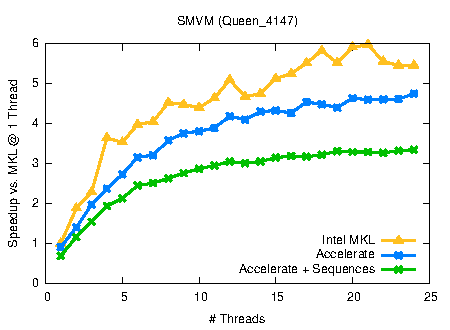
\includegraphics[width=0.8\textwidth]{benchmarks/smvm/figs/smvm.pdf}
\caption{SMVM of Queen\_4147 dataset}
% comparing this work (Accelerate+Sequences) to the prior work
% (Accelerate) and a reference implementation (Intel MKL) on the CPU.}
\label{fig:smvm_queen4147}
\end{figure}

\section{Audio processor}

The audio processing benchmark tests the algorithm described in
Section~\ref{sec:streaming}, computing the @zc_stream@ part of the algorithm
which processes the input audio data along a sliding window. Since standard
Accelerate is limited to flat data parallelism only, it
can only take advantage of a single source of parallelism, and applies the
@processWindow@ operation to a single element of the stream at a time.
% Standard Accelerate is limited to applying the computation to a single
% data window at once, since it is restricted to flat data parallelism only.
However, with sequences, we can also take advantage of another source of
parallelism and process multiple windowed elements at a time.
% However with Sequences we can express the computation over the entire audio
% stream, and the runtime is free to batch several windowed elements to be
% processed together.
This is particularly important for the GPU, since we must have enough work to
fully saturate all the cores of the device, as well as to amortize the overhead
of streaming data between the CPU and GPU\@. On our test machine the runtime
chooses to process 512 elements at a time on the GPU, resulting in a speedup of
$3.3\times$ over regular Accelerate.

Figure~\ref{fig:zero-crossings} shows the strong scaling performance compared to
the implementation in regular Accelerate\footnote{Unfortunately we do not have a
parallel reference implementation of the algorithm to compare to.} on the CPU\@.
As seen in the other benchmark programs, our implementation currently has some
overhead compared to regular Accelerate (which has had more time to mature).
However, since we can also take advantage of the extra parallelism of processing
multiple windowed elements in parallel, we are able to make up the difference in
this benchmark.

% Compared to when executed on the GPU,
% there is enough parallelism within each processing window already to saturate
% the cores already, without needing to also process multiple windows in parallel,

% \tlm{I haven't mentioned CPU results here because they basically aren't very
% good ---either absolute runtime or the selected chunk size, which I could not get
% to stabilise--- but earlier in the prose we did use this to discuss performance
% portability, so...}
% \tlm{the strong scaling graph for regular accelerate vs sequences looks pretty
% good though, so we could include that. An example is in the numbers file. it is
% just that the absolute performance is bad...}

\begin{figure}
\centering
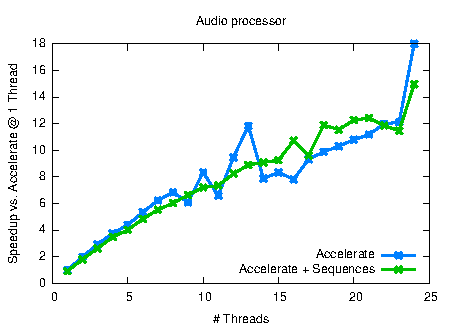
\includegraphics[width=0.8\textwidth]{benchmarks/zero-crossings/figs/zero-crossings.pdf}
\caption{Audio processor}
\label{fig:zero-crossings}
\end{figure}


\section{MD5 Hash}

The MD5 message-digest algorithm~\cite{Rivest:MD5} is a cryptographic hash
function producing a 128-bit hash value that can be used for cryptographic and
data integrity applications. The MD5 benchmark attempts to find the plain text
of an unknown hash with a database of known plaintexts.
%
% ; for each plaintext entry in the
% dictionary, we compute the hash of that entry and compare it to the unknown.
%
We compare to Hashcat,\footnote{\url{https://hashcat.net/hashcat/}} the
self-proclaimed world's fastest CPU-based password recovery tool. Results from
Hashcat are as reported by its inbuilt benchmark mode.

Our sequences based implementation achieves a maximum throughput of 50 million
words per second, compared to Hashcat at 287Mword/sec and standard Accelerate at
155Mword/sec. One key difference between our version using sequences and the
implementation in standard Accelerate is that we stream in and process small
chunks of the input dictionary at a time, rather than loading the entire
database into memory at once. However, our runtime system currently does not
overlap computation with pre-loading the next chunk of input into memory, which
would help close this performance gap. The strong scaling graph is shown in
Figure~\ref{fig:hashcat}.

\begin{figure}
\centering
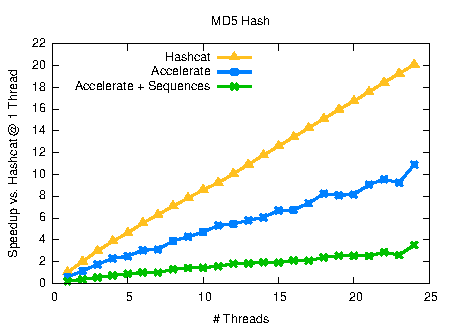
\includegraphics[width=0.8\textwidth]{benchmarks/hashcat/figs/hashcat.pdf}
\caption{MD5 hash recovery}
\label{fig:hashcat}
\end{figure}

\section{PageRank}

PageRank~\cite{Page:pagerank} is a link analysis algorithm which
estimates the relative importance of each element of a linked set of documents. As
input we use a link graph of Wikipedia (English) consisting of 5.7 million pages
and 130 million links. Figure~\ref{fig:pagerank} compares the performance
against an implementation written in Repa~\cite{Keller:Repa,Lippmeier:Guiding},
a data-parallel array programming language similar to Accelerate. Both
Accelerate and Repa represent the link graph as index pairs @(Int,Int)@. While
this representation is not as space efficient as an adjacency list, it is the
one typically chosen for this algorithm as it is more suitable for parallelism.

\begin{figure}
\centering
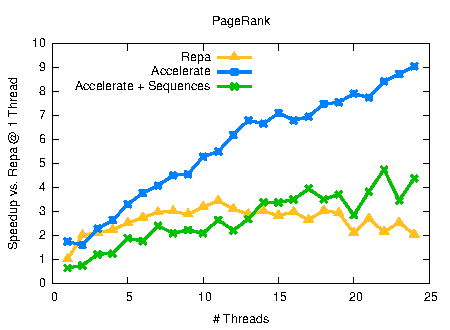
\includegraphics[width=0.8\textwidth]{benchmarks/pagerank/figs/pagerank.pdf}
\caption{PageRank analysis of Wikipedia (English)}
\label{fig:pagerank}
\end{figure}


\chapter{Conclusion}

In this work we argue that adding even one level of nesting to array programs offers considerable benefits to modularity. Moreover, if that form of nesting is in sequences we get the additional benefit of reduced memory constraints.

In Chapter~\ref{chap:motivation} we present the irregular array sequence as an abstract structure and how it adds an additional layer of expressiveness to the array language Accelerate. Even with a relatively small set of operations on sequences, we can express programs that were awkward and non-modular to write before. As well as programs that would otherwise require specific knowledge of the hardware to write without exhausting available GPU memory.

In Chapter~\ref{chap:theory} we describe a novel extension to Blelloch's flattening transform, that we have used to enable irregular arrays sequences, but which can be applied more generally to all nested array structures. This extension is able to identify computations which are regular and generate code that is optimal for that regularity while generating conventional flattened array code for irregular computations.

In Chapter~\ref{chap:enhancements} we describe two further novel components of our work. We introduce the Accelerate Foreign Function Interface (FFI), a new way of allowing for an embedded language to support foreign functions. We also introduce a method of garbage collection that allows for GPU memory to be treated like a cache for arrays that are used in GPU computations.

Finally, Chapter~\ref{chap:Evaluation} evaluates our work with a series of benchmarks.

\section{Contribution}

The work contains 2 major contributions and 2 minor contributions. The two major ones are regularity identifying flattening and irregular array sequences. They are closely related as the former is necessary to implement the latter with expected performance gains. However, it is much more widely applicable. Regularity identifying flattening can be applied to any context where efficient nested arrays are needed.

The minor contributions further extend what we can practically express in an array language, by dynamically reducing memory usage through GPU-aware garbage collection and by giving access to highly-optimised 3rd party libraries through a foreign function interface.

\subsection{Regularity identifying flattening}

While program flattening via Blelloch's flattening transform is well understood, languages that implement it have either assumed everything is irregular~\cite{Blelloch:nesl1995,bergstrom:ndp2gpu,Chakravarty:DPH,Fluet:2007:manticore,proteus-frontiers95}, or, more recently, that everything is regular~\cite{Henriksen:2017futhark}. While the former is most general, it misses opportunities to take advantage of efficiency of regular scheduling. The latter, however, is unable to express irregular computations.

By having a flattening transform that is able to identify regular (sub)programs and generate flat array code for them, while still the flat array code suitable for irregular structures otherwise, we get the best of both worlds. This enable us to support not only irregular nested programs and regular nested programs, but also programs that combine both.

\subsection{Irregular array sequences}

Given two, almost entirely independent, limitations on flat array programs, in this work we show that both can be overcome with the addition of one feature. Irregular sequences of arrays allow us to tk the loss of modularity in flat array programs, without having to tk the challenges of more deeply nested structures. Moreover, they gives us portability between GPUs and CPUs, in particular, their different memory limitations. The same program can be executed on both architectures and, even if the GPU does not have sufficient memory to perform the computation in-core, it will have tk performance on both.

\subsection{GPU-aware garbage collection}

A feature that is useful for both sequence programs and array programs alike is for the garbage collector to be aware of the GPU and its, typically, much smaller memory than the main memory of the system it is in. While the CPU is able to swap pages out to disk, prior to our work, there was no was no system for swapping memory out of the GPUs memory to host memory. By both hooking into GHC's garbage collector, and keeping track of what arrays are in GPU memory, we are able to dynamically manage the memory of the GPU such that the programmer no longer has to concern themselves with exhausting it. A high-level language should abstract away such details. With our work, a programmer only has to concern themselves with whether individual arrays will fit in GPU memory, not whatever the working memory of their program is, which is typically much harder.

\subsection{A Foreign Function Interface for an embedded language}

Foreign function interfaces have proven to be invaluable to the adoption of high-level languages\cite{Chakravarty:haskell-ffi}. Prior to our work, this was an area unexplored in the domain of embedded languages. By introducing an FFI to Accelerate, we made it possible to call out to already highly-optimised low-level libraries from within high-level programs. In addition, different backends can be supported by having different foreign functions for each backend.

\section{Future work}

What we describe in this dissertation could be extended in a number of different ways. Here, we present a few key research possibilities.

\subsection{More sequence operations}

Even though we can express realistic sequence programs with the operations we have, like with different array combinators there is room for more elaborate sequence combinators. In our work, we wanted to avoid the problem of unbounded buffers, but if such a restriction were relaxed (say by supporting data structures that allow for fast concatenation) a much wider range of operations is possible.

\TODO{Example?}

\subsection{More nested structures}

Given the regularity identifying flattening transform in Chapter~\ref{chap:theory} an obvious piece of future work is to support arbitrary nested arrays in Accelerate. While we have demonstrated that it is possible to do so in a way that takes advantage of regularity, there are still questions that arise. In particular, scheduling of deeply nested programs on GPUs has proven to be challenging\cite{bergstrom:ndp2gpu}. Additionally, to really support nested structures, sum and recursive data types are needed. This can be achieved, in a limited fashion, with such types in the meta language, but if that is sufficient or whether Accelerate itself needs them is still an open question.

\subsection{Multi-GPU parallelism}

With sequences, we introduce a new level of parallelism. We've already shown how pipeline parallelism can be used to take advantage of both the CPU and GPU by executing two different stages at the same time, one on the GPU and one on the CPU. However, doing this on multiple GPUs is yet to be explored. It's already possible, with Accelerate's existing support for multiple GPUs, to manually schedule different computations on different GPUs, but to do so automatically is unexplored. Being able to define a sequence pipeline and have the different stages allocated across the available GPUs in such a way as to maximise efficiency (both in terms of work and in terms of data transfer) would be a powerful language feature.

\cleardoublepage
\stopthumb
\backmatter
\let\chapter\oldchapter

\cleardoublepage
\phantomsection
\addcontentsline{toc}{chapter}{Bibliography}
\bibliography{thesis}

\markboth{}{}
\pagebreak
\phantomsection

\vspace*{\stretch{1}}
Copyright 2013-2018 \copyright\ Robert Clifton-Everest


\end{document}